%MIT License
%
%Copyright (c) 2018 Chen Wang [https://chenwang.site]
%
%Permission is hereby granted, free of charge, to any person obtaining a copy
%of this software and associated documentation files (the "Software"), to deal
%in the Software without restriction, including without limitation the rights
%to use, copy, modify, merge, publish, distribute, sublicense, and/or sell
%copies of the Software, and to permit persons to whom the Software is
%furnished to do so, subject to the following conditions:
%
%The above copyright notice and this permission notice shall be included in all
%copies or substantial portions of the Software.
%
%THE SOFTWARE IS PROVIDED "AS IS", WITHOUT WARRANTY OF ANY KIND, EXPRESS OR
%IMPLIED, INCLUDING BUT NOT LIMITED TO THE WARRANTIES OF MERCHANTABILITY,
%FITNESS FOR A PARTICULAR PURPOSE AND NONINFRINGEMENT. IN NO EVENT SHALL THE
%AUTHORS OR COPYRIGHT HOLDERS BE LIABLE FOR ANY CLAIM, DAMAGES OR OTHER
%LIABILITY, WHETHER IN AN ACTION OF CONTRACT, TORT OR OTHERWISE, ARISING FROM,
%OUT OF OR IN CONNECTION WITH THE SOFTWARE OR THE USE OR OTHER DEALINGS IN THE
%SOFTWARE.
\documentclass[12pt,a4paper]{Thesis} % Paper size, default font size and one-sided paper

\graphicspath{%
	{./Pictures/}%
	{./Figures/}%
}
\DeclareMathOperator{\Tr}{Tr}
\let\savedegree\degree
\let\degree\relax
\let\savedegree\ref
\let\rem\relax
%\usepackage{adjustbox}
%\usepackage{amsmath}
%\usepackage[amssymb]{SIunits}
%\usepackage{amssymb}
%\usepackage{multirow}
%\usepackage{wrapfig}
%\usepackage{enumitem}
%\usepackage{subcaption}
%\usepackage{mathtools}
%\usepackage[ruled,vlined,noresetcount]{algorithm2e}
%%\usepackage{algpseudocode}
\usepackage[square, numbers, comma, sort&compress]{natbib} % Use the natbib reference package - read up on this to edit the reference style; if you want text (e.g. Smith et al., 2012) for the in-text references (instead of numbers), remove 'numbers'



\title{\ttitle} % Defines the thesis title - don't touch this

%extra packages
%\usepackage{float}
%\usepackage{color,soul}               % highlighting text
%\usepackage{enumerate}
%\usepackage{Styles/mydefs}
%%% macros.tex
%%% Import packages, define utility commands and define macros
%%% Version 1.1.0

%%%----------
%%% Imports

%%% Text Formatting
\usepackage{xspace}
\usepackage{xcolor}
\usepackage{graphicx}
\usepackage[normalem]{ulem} % normalem do not replace \emph to underline
%\usepackage{amsmath, amssymb, amsfonts}
\usepackage{enumitem}
\usepackage{microtype}
\usepackage{hyphenat}
%%% Reference, Citation and Link
%\usepackage[hyphens]{url}
%\usepackage{url}
%\usepackage[hidelinks]{hyperref}
%\usepackage[hyphens]{url}
\usepackage[anythingbreaks]{breakurl}
%\usepackage{cite}

%%% Tables
\usepackage{booktabs}
\usepackage{multirow}
\usepackage{makecell}
\usepackage{ragged2e}
\usepackage{longtable}
\usepackage{diagbox}
%%% Plots
\usepackage{caption}
% \usepackage{subcaption}
\usepackage{subfloat}
% \usepackage{subfig}
%\usepackage[caption=false]{subfig}
\usepackage{wrapfig}
% Code
\usepackage{listings}

%\usepackage[margin=25mm, a4paper, showframe]{geometry}
\usepackage[many]{tcolorbox}
\usepackage{lipsum}

% Proof
\usepackage{bussproofs}
\usepackage{stackengine}

% Tikz Figs
\usepackage{pifont}
\usepackage{tikz}
%\usepackage{pgf-umlsd} % for flow diagram
\usetikzlibrary{calc}
\usetikzlibrary{shapes.geometric}
\usetikzlibrary{decorations.pathreplacing}
\usetikzlibrary{positioning}
\usetikzlibrary{calc}
\usetikzlibrary{arrows}
\usetikzlibrary{shadows}
%\usetikzlibrary{shapes}

%%% Miscellaneous
\usepackage{balance}
%\usepackage{flushend} % balance the end of double column document
\usepackage{datetime} % for getting current date time

\usepackage[capitalize]{cleveref}
\crefname{section}{Sect.}{Sects.}
\Crefname{section}{Section}{Sections}

%%%----------
%%% Utility Commands
%\renewcommand\footnotetextcopyrightpermission[1]{}
%\settopmatter{printacmref=false}

\setlength{\abovedisplayskip}{5pt}
\setlength{\belowdisplayskip}{5pt}
\setlength{\abovecaptionskip}{5pt}
\setlength{\belowcaptionskip}{5pt}
\setlength{\textfloatsep}{5pt}
\setlength{\floatsep}{5pt}
\setlength{\intextsep}{5pt}
\setlength{\dbltextfloatsep}{5pt}
\setlength{\dblfloatsep}{5pt}

\newcommand{\XSpace}[1]{}
\newcommand{\XComment}[1]{}
\newcommand{\yi}[1]{\textcolor{purple}{Yi: #1}}
\newcommand{\liu}[1]{\textcolor{red}{Liu Ye: #1}}
\newcommand{\lsw}[1]{\textcolor{blue}{Shang-Wei: #1}}
\newcommand{\xh}[1]{\textcolor{cyan}{#1}}
\newcommand{\pn}[1]{\textcolor{blue}{PN: #1}}
\newcommand{\Fix}[1]{\textcolor{red}{#1}}
\newcommand{\Blue}[1]{\textcolor{blue}{#1}}
\newcommand{\EditAdd}[1]{\textcolor{green}{[#1]}}
\newcommand{\EditRm}[1]{\textcolor{red}{[\sout{#1}]}}
\newcommand{\EditMod}[2]{\textcolor{red}{[\sout{#1}]}\textcolor{green}{[#2]}}
\newcommand{\DefMacro}[2]{\expandafter\newcommand\csname rmk-#1\endcsname{#2}}
\newcommand{\UseMacro}[1]{\csname rmk-#1\endcsname}

\newcommand{\CZComment}[1]{\Fix{#1}}

\renewcommand{\paragraph}[1]{\vskip 0.05in \noindent\textbf{#1.}}
\newcommand{\MyParaOnly}[1]{\noindent\textbf{#1}}
\newcommand{\Answer}[1]{\subsection{#1}}
\newcommand{\reducedstrut}{\vrule width 0pt height .9\ht\strutbox depth .9\dp\strutbox\relax}
\newcommand{\InputWithSpace}[1]{\bgroup\def\arraystretch{1.1}\input{#1}\egroup}
\newcommand{\Code}[1]{{\ifmmode{\mathtt{#1}}\else$\mathtt{#1}$\fi}}
\newcommand{\CodeIn}[1]{{\ifmmode{\mathtt{#1}}\else$\mathtt{#1}$\fi}}
\newcommand{\ColorBack}[1]{%
  \begingroup
  \setlength{\fboxsep}{0pt}%
  \colorbox{purple!20}{\reducedstrut#1\/}%
  \endgroup
}

\DeclareMathOperator*{\argmax}{arg\,max}
%\newcommand{\tool}{\textsc{FairCon}\xspace}
\newcommand{\faircon}{\textsc{FairCon}\xspace}
\newcommand{\modcon}{\textsc{ModCon}\xspace}
\newcommand{\spcon}{\textsc{SpCon}\xspace}
\newcommand\overhead[2]{\mathrel{\overset{\makebox[0pt]{\mbox{\normalfont\tiny\sffamily
$#2$}}}{#1}}}
\newcommand{\mand}{\texttt{\textbf{ and }}\xspace}
\newcommand{\mnot}{\texttt{\textbf{not }}\xspace}
\newcommand{\mtrue}{\texttt{\textbf{true }}\xspace}
\newcommand{\report}{\ensuremath{\hat{\theta}}\xspace}


%% \newcommand{\historyslicing}{history slicing\xspace}
%% \newcommand{\historyslice}{history slice\xspace}
%% \newcommand{\historyslices}{history slices\xspace}
%% \newcommand{\changehistory}{change history\xspace}
%% \newcommand{\ChangeHistory}{Change History\xspace}
%% \newcommand{\Changehistory}{Change history\xspace}
%% \newcommand{\changehistories}{change histories\xspace}
%% \newcommand{\ChangeHistories}{Change Histories\xspace}
%% \newcommand{\svh}{software change history\xspace}
%% \newcommand{\schangehistory}{software change history\xspace}
%% \newcommand{\schangehistories}{software change histories\xspace}
%% \newcommand{\svhs}{software change histories\xspace}
%% \newcommand{\Svhs}{Software change histories\xspace}
%% \newcommand{\Schangehistories}{Software change histories\xspace}

%% \newcommand{\subseq}{\vartriangleleft}
%% \newcommand{\pfun}{\mathrel{\ooalign{\hfil$\mapstochar\mkern5mu$\hfil\cr$\to$\cr}}}
%% \newcommand{\nat}{\mathbb{N}\xspace}
%% \newcommand{\tline}[1]{\textsc{Text}\ensuremath{(#1)}\xspace}
%% \newcommand{\astree}[1]{\textsc{Ast}\ensuremath{(#1)}\xspace}
%% \newcommand{\troot}[1]{\textsc{Root}\ensuremath{(#1)}\xspace}
%% \newcommand{\parent}[1]{\textsc{Parent}\ensuremath{(#1)}\xspace}
%% \newcommand{\leaf}[1]{\textsc{Leaf}\ensuremath{(#1)}\xspace}

%% \newcommand{\fields}[1]{\textsc{Fields}\ensuremath{(#1)}\xspace}
%% \newcommand{\methods}[1]{\textsc{Methods}\ensuremath{(#1)}\xspace}
%% \newcommand{\subtype}{\ensuremath{<:}}
%% \newcommand{\emptyseq}{\ensuremath{\langle\rangle}\xspace}

%% \DeclareRobustCommand{\lset}[1]{\ifthenelse{\equal{#1}{}}{\ensuremath{\Delta}}%
%%   {\ensuremath{\Delta(#1)}\xspace}}
%% \DeclareRobustCommand{\tset}[1]{\ifthenelse{\equal{#1}{}}{\ensuremath{\hat{\Delta}}}%
%%   {\ensuremath{\hat{\Delta}(#1)}\xspace}}

%% \DeclareRobustCommand{\ledit}[1]{\ifthenelse{\equal{#1}{}}%
%%   {\ensuremath{\delta}\xspace}%
%%   {\ensuremath{\delta(#1)}\xspace}}

%% \DeclareRobustCommand{\tedit}[1]{\ifthenelse{\equal{#1}{}}%
%%   {\ensuremath{\hat{\delta}}\xspace}%
%%   {\ensuremath{\hat{\delta}(#1)}\xspace}}

%% \newcommand{\ins}[1]{\ifthenelse{\equal{#1}{}}{\textsc{Ins}\xspace}%
%%   {\textsc{Ins}\ensuremath{(#1)}\xspace}}
%% \newcommand{\del}[1]{\ifthenelse{\equal{#1}{}}{\textsc{Del}\xspace}%
%%   {\textsc{Del}\ensuremath{(#1)}\xspace}}
%% %\newcommand{\mov}[1]{\textsc{Mov}\ensuremath{(#1)}\xspace}
%% \newcommand{\upd}[1]{\ifthenelse{\equal{#1}{}}{\textsc{Upd}\xspace}%
%%   {\textsc{Upd}\ensuremath{(#1)}\xspace}}

%% \newcommand{\INS}[1]{\ifthenelse{\equal{#1}{}}{\textsc{Ins}\xspace}%
%%   {\textsc{Ins}\texttt{(#1)}\xspace}}
%% \newcommand{\DEL}[1]{\ifthenelse{\equal{#1}{}}{\textsc{Del}\xspace}%
%%   {\textsc{Del}\texttt{(#1)}\xspace}}
%% \newcommand{\UPD}[1]{\ifthenelse{\equal{#1}{}}{\textsc{Upd}\xspace}%
%%   {\textsc{Upd}\texttt{(#1)}\xspace}}

%% \newcommand{\val}[1]{\ifthenelse{\equal{#1}{}}{\ensuremath{\nu}}%
%%   {\ensuremath{\nu(#1)}}\xspace}
%% \newcommand{\ide}[1]{\ifthenelse{\equal{#1}{}}{\ensuremath{id}}%
%%   {\ensuremath{id(#1)}}\xspace}
%% \newcommand{\lab}[1]{\ifthenelse{\equal{#1}{}}{\ensuremath{\iota}}%
%%   {\ensuremath{\iota(#1)}}\xspace}

\definecolor{silver}{RGB}{192,192,192}
\newcommand{\HighlightCode}[1]{\hspace{-3pt}\colorbox{silver}{#1\vphantom{-}}}

% for table headers
\newcommand{\specialcell}[2][c]{%
  \begin{tabular}[#1]{@{}c@{}}#2\end{tabular}}
\newcolumntype{R}[1]{>{\RaggedLeft\arraybackslash}p{#1}}
\newcolumntype{L}[1]{>{\RaggedRight\arraybackslash}p{#1}}

\newcommand{\cmark}{\ding{51}}
\newcommand{\xmark}{\ding{55}}

%\input{defs-logic} % for logic symbols
%\input{defs-code} % for code listings

% for including revision info in the document
\newcommand{\RevisionInfo}{\Fix{Time: \today{} at \currenttime{.}}}


%%%----------
%%% Macros
%\newcommand{\UPPERCASE}{Title Case\xspace}
%\newcommand{\Firstcap}{First cap\xspace}
%\newcommand{\lowercase}{lower case\xspace}

\newcommand{\MCr}{Maven Central repository\xspace}
\newcommand{\MCR}{Maven Central Repository\xspace}
\newcommand{\github}{GitHub\xspace}
%\newcommand{\stackoverflow}{StackOverflow\xspace}

\newcommand{\df}{differential fact\xspace}
\newcommand{\dfs}{differential facts\xspace}
\newcommand{\old}{original\xspace}
\newcommand{\new}{upgraded\xspace}
\newcommand{\Old}{Original\xspace}
\newcommand{\New}{Upgraded\xspace}
\newcommand{\grok}{Grok\xspace}
\newcommand{\evosuite}{\textsc{EvoSuite}\xspace}
\newcommand{\lib}{library\xspace}
\newcommand{\Lib}{Library\xspace}
\newcommand{\client}{client\xspace}
\newcommand{\Client}{Client\xspace}
\newcommand{\difffacts}{inter-version facts\xspace}
\newcommand{\depsfacts}{intra-version facts\xspace}
\newcommand{\cslicer}{\textsc{CSlicer}\xspace}
\newcommand{\definer}{\textsc{Definer}\xspace}
\newcommand{\clltuple}{$\langle cli,$\allowbreak$lib,$\allowbreak$lib'\rangle$\xspace}
\newcommand{\bcel}{Apache BCEL\xspace}
\newcommand{\compatibilitytesting}{upgrade compatibility checking\xspace}
\newcommand{\CompatibilityTesting}{Upgrade Compatibility Checking\xspace}
\newcommand{\oldlibsym}{$lib$\xspace}
\newcommand{\newlibsym}{$lib'$\xspace}
\newcommand{\clientsym}{$cli$\xspace}

\newcommand{\NumOfSlicingSubjects}{10\xspace}
\newcommand{\dosc}{\textsc{DoSC}\xspace}
\newcommand{\setoftests}{set of tests\xspace}
\newcommand{\NumOfSlicingProjects}{eight\xspace}

\newcommand{\NumOfSubjectsInRTSDataset}{408\xspace}
\newcommand{\NumOfCompatSubjects}{ten\xspace}
\newcommand{\NumOfSubjectsHaveCompatIssues}{four\xspace}
\newcommand{\NumOfSubjectsNotHaveCompatIssues}{six\xspace}
\newcommand{\MaxReduce}{99.11\%\xspace}
\newcommand{\MinReduce}{27.37\%\xspace}
\DefMacro{NumOfSubjectsReduceOver90Percent}{seven}

%% Tables
%Symbols for relations
\newcommand{\rCov}{\ensuremath{\mathit{Cov}}\xspace}
\newcommand{\rIns}{\ensuremath{\mathit{Ins}}\xspace}
\newcommand{\rUpd}{\ensuremath{\mathit{Upd}}\xspace}
\newcommand{\rDel}{\ensuremath{\mathit{Del}}\xspace}
\newcommand{\rCall}{\ensuremath{\mathit{Call}}\xspace}
\newcommand{\rRef}{\ensuremath{\mathit{Ref}}\xspace}
\newcommand{\rContain}{\ensuremath{\mathit{Contain}}\xspace}
\newcommand{\rParent}{\ensuremath{\mathit{Parent}}\xspace}
\newcommand{\rHunk}{\ensuremath{\mathit{Hunk}}\xspace}
\newcommand{\rCmt}{\ensuremath{\mathit{Cmt}}\xspace}

% Compat Subjects Table
\newcommand{\TableCaptionCompatSubjects}{Subjects of \CompatibilityTesting Experiment (All URLs Start with https://github.com/)\label{tab:compat:subjects}}
\newcommand{\TableHeadSubjectId}{\textbf{ID}}
\newcommand{\TableHeadClient}{\textbf{Client}}
\newcommand{\TableHeadLib}{\textbf{Library}}
\newcommand{\TableHeadSHA}{\textbf{SHA}}
\newcommand{\TableHeadURL}{\textbf{URL}}
\newcommand{\TableHeadLibOldVer}{\textbf{$Lib$ Version}}
\newcommand{\TableHeadLibNewVer}{\textbf{$Lib'$ Version}}

% Compat Results Table
%% \newcommand{\TableCaptionCompatResults}{Results of Compatibility Testing Experiment (\#CC=the Number of Client Classes; \#QC=the Number of Client Classes Influenced by the Upgrade, obtained by querying Factbase; \%Red=Reduction Rate=(\#CC-\#QC)/\#CC; \#T=the Number of Generated Test Classes; \#FT=the Number of Generated Test Classes that Flip from Pass to Fail after \Lib Upgrade)\label{tab:compat:results}}
\newcommand{\TableCaptionCompatResults}{Results of \CompatibilityTesting Experiment\label{tab:compat:results}}
\newcommand{\TableHeadNumOfAllClasses}{\textbf{\#CC}}
\newcommand{\TableHeadNumOfAffectedClasses}{\textbf{\#AC}}
\newcommand{\TableHeadReduction}{\textbf{\%Reduction}}
\newcommand{\TableHeadNumOfGeneratedTestClasses}{\textbf{\#T}}
\newcommand{\TableHeadNumOfFailedTestClasses}{\textbf{\#FT}}

%% Numbers

%\input{tables/icse2020-compat-subjects-numbers}
%\input{tables/icse2020-compat-result-numbers}

%%%----------
%%% Package settings

% code listing style
\lstdefinestyle{tafile}{%
    basicstyle=\scriptsize\ttfamily,
    %basicstyle=\large,
    frame=single,
    rulecolor=\color{black},
    morekeywords={\$INHERIT, Update, Insert, Delete, reference, contain, call, HunkDep, Coverage},
    tabsize=2,
    numbers=left,                    % where to put the line-numbers; possible values are (none, left, right)
    numbersep=5pt,                   % how far the line-numbers are from the code
    stepnumber=1,
    numberstyle=\tiny\color{gray},   % the style that is used for the line-numbers
    keywordstyle=\sffamily,
}

\lstdefinestyle{syntax}{%
    basicstyle=\small\ttfamily,
    backgroundcolor=\color{white},
    escapeinside={(*}{*)},
    frame=none,
    morekeywords={,id,bid,valuation,allocation,price,max,argmax,}
    tabsize=2,
    numbers=none,                    % where to put the line-numbers; possible values are (none, left, right)
    keywordstyle=\bfseries\color{black}\sffamily,
}
%%% rq box
\newtcolorbox{rqbox}[1]{%
    tikznode boxed title,
    enhanced,
    arc=0mm,
    boxrule=0.5pt,
    interior style={white},
    attach boxed title to top center= {yshift=-\tcboxedtitleheight/2},
    colbacktitle=white,coltitle=black,
    boxed title style={size=normal,colframe=white,boxrule=0pt},
    title=\textbf{Answer to }{\textbf{#1}}}
\newcommand{\prefer}{\vartriangle}
\newcommand{\announce}{\triangledown}
\newcommand{\join}{\oplus}
\newcommand{\associate}{\barwedge}
\newcommand{\reduce}{ \mapsto}
\newcommand{\fourspace}{\xspace\xspace\xspace\xspace}
\newcommand{\twospace}{\xspace\xspace}
\newcommand{\terminate}{\Gamma}
\newcommand{\expand}{::=}
\newcommand{\N}{\mathbb{N}}
\newcommand{\R}{\mathbb{R}}
\newcommand{\Octon}{\mathbb{O}}
\newcommand{\Z}{\mathbb{Z}}
%\hypersetup{draft}

\definecolor{codegreen}{rgb}{0,0.6,0}
\definecolor{codegray}{rgb}{0.5,0.5,0.5}
\definecolor{codepurple}{rgb}{0.58,0,0.82}
\definecolor{backcolour}{rgb}{0.95,0.95,0.92}

\lstdefinestyle{mystyle}{
    backgroundcolor=\color{backcolour},
    commentstyle=\color{codegreen},
    keywordstyle=\color{magenta},
    numberstyle=\tiny\color{codegray},
    stringstyle=\color{codepurple},
    basicstyle=\ttfamily\footnotesize,
    breakatwhitespace=false,
    breaklines=true,
    captionpos=b,
    keepspaces=true,
    numbers=left,
    numbersep=5pt,
    showspaces=false,
    showstringspaces=false,
    showtabs=false,
    tabsize=2
}
\lstset{style=mystyle}

\usepackage{alphabeta}
\newcommand{\ra}[1]{\renewcommand{\arraystretch}{#1}}
%\usepackage[group-separator={,}]{siunitx}

%
%	ModCon Macros
%
\usepackage{caption}
\usepackage{subcaption}
\newcommand{\code}[1]{\texttt{#1}}
\newcommand{\modconurl}{https://sites.google.com/view/modcon}
\newcommand{\cfg}{control flow graph\xspace}
\newcommand{\company}{WeBank\xspace}
\newcommand{\wecredit}{CMA\xspace}

%  FairCon Macros
\usepackage{siunitx}

\begin{document}



\frontmatter % Use roman page numbering style (i, ii, iii, iv...) for the pre-content pages

\setstretch{1.3} % Line spacing of 1.3
% Define the page headers using the Fr package and set up for one-sided printing

\pagestyle{fancy} % Finally, use the "fancy" page style to implement the FancyHdr headers
\fancyhead{}   %clear all fields
\fancyhead[LO]{\sl{\leftmark}}
\fancyhead[RE]{\sl{\rightmark}}
\fancyhead[LE,RO]{\thepage}


%----------------------------------------------------------------------------------------
%	TITLE PAGE
%----------------------------------------------------------------------------------------

%%% Use \maketitleforreview instead of \maketitle, if you want a PLAIN TITLE PAGE

\maketitle
%\maketitleforreview


% % ----------------------------------------------------------------------------------------
% % 	DECLARATION PAGE
% % ----------------------------------------------------------------------------------------

% \thesisdeclareOriginality{I hereby certify that the work embodied in this thesis is the result of original research, is free of plagiarised materials, and has not been submitted for a higher degree to any other University or Institution.}{Aug. 2018}{Styles/signature.png}

% \thesisdeclareSupervisor{I have reviewed the content and presentation style of this thesis and declare it is free of plagiarism and of sufficient grammatical clarity to be examined.  To the best of my knowledge, the research and writing are those of the candidate except as acknowledged in the Author Attribution Statement. I confirm that the investigations were conducted in accord with the ethics policies and integrity standards of Nanyang Technological University and that the research data are presented honestly and without prejudice.}{Mar. 2019}{Styles/signature.png}

% \thesisdeclareAuthorship{Please select one of the following; *delete as appropriate:
% \\
% *(A) This thesis does not contain any materials from papers published in peer-reviewed journals or from papers accepted at conferences in which I am listed as an author.
% \\
% *(B) This thesis contains material from [x number] paper(s) published in the following peer-reviewed journal(s) / from papers accepted at conferences in which I am listed as an author.}
% {Please amend the typical statements below to suit your circumstances if (B) is selected.

% 	Chapter 4 is published as {\color{blue}D.T. Murphy, S. Schmid, J.R. Hester, P.E.R. Blanchard, and W. Miiller.  Coordination site disorder in spinel-type LiMnTiO4.  Inorganic Chemistry 54, 4636-4643 (2015). DOI: 10.1021/ic502747p.}

% 	The contributions of the co-authors are as follows:
% 	\begin{itemize}[topsep=1pt,itemsep=1pt,partopsep=1pt, parsep=1pt]
% 		\item A/Prof Schmid provided the initial project direction and edited the manuscript drafts.
% 		\item I prepared the manuscript drafts.  The manuscript was revised by Dr Hester and Dr. Blanchard.
% 		\item I co-designed the study with A/Prof Siegbert Schmid and performed all the laboratory work at the School of Materials Science and Engineering and the Singapore Synchrotron Light Source.   I also analyzed the data.
% 		\item All microscopy, including sample preparation, was conducted by me in the Facility for Analysis, Characterization, Testing and Simulation.
% 		\item Dr James Hester assisted in the collection of the neutron powder diffraction data.
% 		\item Dr Peter Blanchard assisted in the interpretation of the X-ray absorption spectroscopy data and carried out the spectral interpretation.
% 		\item Dr Wojciech Miiller assisted in the collection and provide guidance in the interpretation of the magnetic measurement data.
% 	\end{itemize}

% 	Chapter 5 is published as {\color{blue}H. V Doan, B. Yao, Y. Fang, A. Sartbaeva, U. Hintermair, V. P Ting, Controlled Formation of Hierarchical Metal-Organic Frameworks using CO2 Expanded Solvent Systems. In press, ACS Sustainable Chemistry \& Engineering (2017). DOI: 10.1021/acssuschemeng.7b01429}

% 	The contributions of the co-authors are as follows:
% 	\begin{itemize}[topsep=1pt,itemsep=1pt,partopsep=1pt, parsep=1pt]
% 		\item Prof Ting suggested the materials area and edited the manuscript drafts.
% 		\item I wrote the drafts of the manuscript.  The manuscript was revised together with Dr. Sartbaeva and Dr. Yao.
% 		\item II performed all the materials synthesis, collected X-ray diffraction patterns and visible light spectra, carried transmission electron microscopy, and conducted data evaluation.
% 		\item IDr. Y. Fang conducted the Rietveld analysis of the powder X-ray diffraction data and single crystal structure determinations.
% 		\item IDr U. Hintermair conducted the molecular dynamics simulations.
% 		\item IMs. A. Sartbaeva prepared the samples for electron microscopy.
% 	\end{itemize}
% }{Mar. 2019}{Styles/signature.png}

% ----------------------------------------------------------------------------------------
% 	ACKNOWLEDGEMENTS
% ----------------------------------------------------------------------------------------

% \setstretch{1.3} % Reset the line-spacing to 1.3 for body text (if it has changed)

% \acknowledgements{\addtocontents{toc}{\vspace{0.8em}} % Add a gap in the Contents, for aesthetics

% I wish to express my greatest gratitude to my advisor.

% % \begin{flushright}
% % \emph{Jinming Xu, December 2015}
% % \end{flushright}
% }

%----------------------------------------------------------------------------------------
%	QUOTATION PAGE
%----------------------------------------------------------------------------------------

% \pagestyle{empty} % No headers or footers for the following pages
% \emph{``If I had one hour to save the world, I would spend 55 minutes defining the problem and only five minutes finding the solution."}

% \begin{flushright}
% ---Einstein, Albert
% \end{flushright}
% \null\vfill % Add some space to move the quote down the page a bit

% \begin{center}
% \large{To my dear family}
% \end{center}
% \vfill\vfill\null % Add some space at the bottom to position the quote just right
% \cleardoublepage % Start a new page and make the next page a right-hand (odd-numbered) page, producing a blank page if necessary

% \pagestyle{fancy} % Return the page headers back to the "fancy" style
% \fancyhead{}   %clear all fields
% \fancyhead[LO]{\sl{\leftmark}}
% \fancyhead[RE]{\sl{\rightmark}}
% \fancyhead[LE,RO]{\thepage}

% %----------------------------------------------------------------------------------------
% %	ABSTRACT PAGE
% %----------------------------------------------------------------------------------------

 \addtotoc{Abstract} % Add the "Abstract" page entry to the Contents

 \abstract{\addtocontents{toc}{\vspace{0.8em}}}% Add a gap in the Contents, for aesthetics

% % 1. The Problem 2. The Issues 3. The Approach 4. The Results 5. The Experiments 6. The Applications

% My abstracts
Smart contracts are stateful computer programs running on blockchain platforms to manage large sums of
cryptocurrency, govern and carry out transactions of assets between multiple parties.
The security of smart contracts has attracted great attention, ever since their adoption in the management of massive cryptocurrency transactions.
However, little work has been done on stateful smart contract applications for its great complexity.
The main challenge lies that most smart contracts are not well specified.
Compared to the security, the fairness issues of smart contracts have not yet attracted much attention. 
However, there is a likely mismatch between the participants' expectations and the actual implementation of contracts.

In this progress report, several solutions are proposed to address these challenges.
An automated verification framework of smart contract fairness is used to help find the mismatch between the user expectations and the contract implementation where contracts are abstracted as games, i.e., mechanism models and the fairness properties originate from game theory as well.
For enterprise smart contracts, they are well specified.
A model-based testing framework is provided to facilitate the testing of these smart contracts.
To overcome the missing of contract specification, our future work aims to learn a likely specification of smart contracts and find user permission bugs via time travel on transaction history. 
A big picture of the framework to enforce both security and fairness of smart contracts also remains to do in the future.
%----------------------------------------------------------------------------------------
%	LIST OF CONTENTS/FIGURES/TABLES PAGES
%----------------------------------------------------------------------------------------

% \pagestyle{fancy} % The page style headers have been "empty" all this time, now use the "fancy" headers as defined before to bring them back

\tableofcontents % Write out the Table of Contents

\listoffigures % Write out the List of Figures

\listoftables % Write out the List of Tables


%----------------------------------------------------------------------------------------
%	ABBREVIATIONS
%----------------------------------------------------------------------------------------

%\clearpage % Start a new page
%
%\setstretch{1.5} % Set the line spacing to 1.5, this makes the following tables easier to read
%
%\lhead{\emph{Abbreviations}} % Set the left side page header to "Abbreviations"
%\listofsymbols{ll} % Include a list of Abbreviations (a table of two columns)
%{
%\textbf{LAH} & \textbf{L}ist \textbf{A}bbreviations \textbf{H}ere \\
%%\textbf{Acronym} & \textbf{W}hat (it) \textbf{S}tands \textbf{F}or \\
%}

%----------------------------------------------------------------------------------------
%	PHYSICAL CONSTANTS/OTHER DEFINITIONS
%----------------------------------------------------------------------------------------

%\clearpage % Start a new page
%
%\lhead{\emph{Physical Constants}} % Set the left side page header to "Physical Constants"
%
%\listofconstants{lrcl} % Include a list of Physical Constants (a four column table)
%{
%Speed of Light & $c$ & $=$ & $2.997\ 924\ 58\times10^{8}\ \mbox{ms}^{-\mbox{s}}$ (exact)\\
%% Constant Name & Symbol & = & Constant Value (with units) \\
%}

%----------------------------------------------------------------------------------------
%	SYMBOLS
%----------------------------------------------------------------------------------------

% \cleardoublepage  % Start a new page (no need if the previous page is list of figures)

% \listofnomenclature{ll} % Include a list of Symbols (a three column table)
% {
% % \multicolumn{2}{l}{\LARGE{\textbf{Symbols}}}\\[0.618cm]
% % $\mathcal{R}^n$                    &the $n$-dimensional Euclidean space\\
% % $\mathcal{H}$                      &the Euclidean  space\\
% % $\norm{\cdot}$                     &the 2-norm of a vector or matrix in Euclidean space\\
% % $\norm{\cdot}_G$                   &the induced norm of a vector in G-space\\
% % $\norm{\cdot}_E$                   &the induced norm of a vector or matrix in probabilistic space\\


% % $\odot$                            &the Hadamard (component-wise) product\\
% % $\otimes$                          &the Kronecker product\\
% % $\innprod{\cdot}{\cdot}$           &the inner product of two vectors\\
% % $\circ$                            &the composition of functions\\ [0.618cm]


% % $\nabla f$                    &the gradient vector\\
% % $\mathcal{C}^k$               &the function with continuous partial derivatives up to $k$ orders\\
% % % $T_x\mathcal{M}$              &the tangent space of the set $\mathcal{M}$\\
% % % $x_i$                         &the $i$-th component of a vector $x$\\
% % $x_{i,k}$                     &the $i$-th component of a vector $x$ at time $k$\\
% % $\bar{x}$                     &the vector with the average of all components of $x$ as each element\\
% % $\ones$                       &all-ones column vector with proper dimension\\
% % $\mathcal{C}$                 &the average space, i.e., $span\{{\bf 1}\}$ \\
% % $\mathcal{C}^\perp$           &the disagreement space, i.e., $span^\perp\{{\bf 1}\}$ \\
% % % W                             &the weight matrix\\
% % % L                             &the Laplacian matrix\\
% % $\Pi_\parallel$               &the projection matrix to the average space $\mathcal{C}$\\
% % $\Pi_\perp$                   &the projection matrix to the disagreement space $\mathcal{C}^\perp$ \\
% % $O(\cdot)$                    &order of magnitude or ergodic convergence rate (running average)\\
% % $o(\cdot)$                    &non-ergodic convergence rate\\
% % % $O(\cdot)$                    &the ergodic convergence rate stated in terms of the running average\\
% % % $o(\cdot)$                    &the non-ergodic convergence rate stated in terms of $x_k$\\
% % $\mathcal{N}_i$               &the index set of the neighbors of agent $i$ \\ [1cm]

% \multicolumn{2}{l}{\LARGE{\textbf{Acronyms}}}\\[0.618cm]
% DOP                      & Distributed Optimization Problem\\
% EDOP                     & Equivalent Distributed Optimization Problem\\
% SDOP                     & Stochastic Distributed Optimization Problem\\
% OEP                      & Optimal Exchange Problem\\
% OCP                      & Optimal Consensus Problem\\
% DOCP                     & Dynamic Optimal Consensus Problem\\[0.618cm]
% AugDGM           & Augmented Distributed Gradient Methods\\
% AsynDGM          & Asynchronous Distributed Gradient Methods\\
% D-ESC            & Distributed Extremum Seeking Control\\
% D-SPA            & Distributed Simultaneous Perturbation Approach\\
% % D-PDSPA & Distributed Primal-Dual Simultaneous Perturbation Approach\\
% D-FBBS           & Distributed Forward-Backward Bregman Splitting\\
% ADMM             & Alternating Direction Method of Multipliers\\
% DSM              & Distributed (Sub)gradient Method\\[0.618cm]

% GAS                      & Globally Asymptotically Stable \\
% UGAS                     & Uniformly Globally Asymptotically Stable \\
% SPAS                     & Semi-globally Practically Asymptotically Stable\\
% USPAS                    & Uniformly Semi-globally Practically Asymptotically Stable\\[0.618cm]
% HoS                      & Heterogeneity of Stepsize\\
% FPR                      & Fixed Point Residual\\
% OBE                      & Objective Error\\[0.618cm]
% i.i.d.           & independent and identically distributed\\
% $a.s.$           & almost sure convergence of a random sequence\\
% }

%----------------------------------------------------------------------------------------
%	DEDICATION
%----------------------------------------------------------------------------------------

%\setstretch{1.3} % Return the line spacing back to 1.3
%
%\pagestyle{empty} % Page style needs to be empty for this page
%
%\dedicatory{For/Dedicated to/To my\ldots} % Dedication text
%
%\addtocontents{toc}{\vspace{2em}} % Add a gap in the Contents, for aesthetics



%----------------------------------------------------------------------------------------
%	AUTHOR'S PUBLICATIONS
%----------------------------------------------------------------------------------------

\authorpublications{
%	
%	\section*{Awards}
%	
%	\begin{itemize}
%		\item \textbf{Best Paper Awards}, ``A Great System,'' \emph{Nature}.
%	\end{itemize}
%	
%	\section*{Patents}
%	\begin{itemize}
%		\item \textbf{A Great System}, ``A Great System,'' \emph{Nature}.
%	\end{itemize}
	
	\section*{Journal Articles}
	
	\begin{itemize}
		\item Wang, Haijun and \textbf{Liu, Ye} and Li, Yi and Lin, Shang-Wei and Artho, Cyrille and Ma, Lei and Liu, Yang, ``Oracle-supported dynamic exploit generation for smart contracts'' \emph{IEEE Transactions on Dependable and Secure Computing}, 2020.
	\end{itemize}
	
	\section*{Conference Proceedings}
%		title={Towards automated verification of smart contract fairness},
%	author={Liu, Ye and Li, Yi and Lin, Shang-Wei and Zhao, Rong},
%	booktitle={Proceedings of the 28th ACM Joint Meeting on European Software Engineering Conference and Symposium on the Foundations of Software Engineering},
%	pages={666--677},
%	year={2020}
	\begin{itemize}
		\item \textbf{Liu, Ye} and Li, Yi and Lin, Shang-Wei and Zhao, Rong, ``Towards automated verification of smart contract fairness'' in \emph{Proceedings of the 28th ACM Joint Meeting on European Software Engineering Conference and Symposium on the Foundations of Software Engineering, 2020}. Accepted.
	\end{itemize}

	\begin{itemize}
		\item \textbf{Liu, Ye} and Li, Yi and Lin, Shang-Wei and Yan, Qiang, `ModCon: a model-based testing platform for smart contracts'' in \emph{Proceedings of the 28th ACM Joint Meeting on European Software Engineering Conference and Symposium on the Foundations of Software Engineering, 2020}. Accepted.
	\end{itemize}
	
}

%----------------------------------------------------------------------------------------
%	THESIS CONTENT - CHAPTERS
%----------------------------------------------------------------------------------------

\mainmatter       % Begin numeric (1,2,3...) page numbering
\pagenumbering{arabic}
\setstretch{1.3}  % Return the line spacing back to 1.3

% define the headings for the body of the thesis
\fancyhead{}   %clear all fields
\fancyhead[LO]{\sl{\leftmark}}
\fancyhead[RE]{\sl{\rightmark}}
\fancyhead[LE,RO]{\thepage}



% Include the chapters of the thesis as separate files from the Chapters folder
% Uncomment the lines as you write the chapters

% \part{Introduction and Background}
%!TEX root=../mythesis.tex
% Chapter 1

\chapter{Introduction} % Main chapter title
\chaptermark{Introduction}
\label{ch:introduction} % For referencing the chapter elsewhere, use \ref{Chapter1} 
%----------------------------------------------------------------------------------------
%	SECTION 1
%----------------------------------------------------------------------------------------
\section{Motivation and Challenge}
Smart contracts are stateful computer programs running on blockchain platforms to manage large sums of
cryptocurrency, govern and carry out transactions of assets between multiple parties.
The blockchain technology has been booming in recent years, since the introduction of Bitcoin~\cite{nakamoto2008bitcoin} by Nakamoto in 2008.
The blockchain networks can be broadly categorized into the permissionless and permissioned blockchains, where the former is open to the public (e.g.,
Bitcoin~\cite{nakamoto2008bitcoin} and Ethereum~\cite{Ethereum}) and the latter is only accessible to trusted groups or private institutions (e.g., Hyperledger Fabric~\cite{hyperledger-fabric} and FISCO BCOS~\cite{fisco}).
The distributed and tamper-resistant nature of blockchain has made it the perfect platform for hosting smart contracts.
Ethereum~\cite{Ethereum} and EOS~\cite{EOS} are the most popular permissionless blockchain platforms which
support smart contracts applicable in many areas.
As of Nov 2020, there are over 1.5 million smart contracts deployed on Ethereum, which is a 100 fold increase since just two years ago.
These smart contracts have enabled about 3.1K decentralized applications (DApps)~\cite{dapp-stats}
serving around 80K daily users on finance, health, governance, gambling, games, etc.


\textcolor{black}{The security of smart contracts} has attracted great attention, ever since their adoption in the management of massive cryptocurrency transactions.
The most notorious attack is that malicious attackers exploited the \emph{reentrancy vulnerability} in the DAO contract on Ethereum~\cite{DAO_attacks}, which resulted in
a loss of \$60 million worth in 2016.
EOS gambling games were intensively hacked in 2019 using a technique called the \emph{transaction congestion attack}~\cite{EOS_attacks} and led
to significant asset loss of smart contract applications such as \texttt{EOS.WIN} and \texttt{EOSPlay}.
The root cause of these attacks is that certain security vulnerabilities introduced during contract development are exploited by malicious parties, causing a loss for the contract owners (and possibly other honest participants).
Most vulnerabilities subject to programming errors, indicating a mismatch between the contract developers' expectations and how the contract code actually works.
Therefore, much research has been dedicated to preventing attacks, discovering and mitigating such vulnerabilities .

\textcolor{black}{However, little work has been done on more enterprise smart contract applications} for its great complexity.
The contract execution on permissionless chains is bounded by limited resource such that smart contracts are often kept simple.
For example, on Ethereum, user has to pay miners (who in charge of executing transactions) a certain amount of ``gas'' (cryptocurrency on Ethereum) as the transaction fee to deploy or interact with contract, which is mainly decided by the computational complexity of contracts (e.g., up to \$15 in fees~\cite{gas-fee}).
Therefore, most permissionless blockchains are mainly used for crytocurrency exchange (e.g., ERC Token and DeFi applications).
In contrast, the permissioned blockchains aim to create real value.
For instance, FISCO BCOS has been successfully adopted in areas such as government and judicial services, supply chain, finance, health care, copyright management, education, transportation, and agriculture~\cite{fisco}.
The smart contracts powering these enterprise applications are more sophisticated and often demonstrate strong stateful behaviors.
However, existing testing and analysis tools~\cite{jiang2018contractfuzzer,oyente,securify,SmartCheck,wang2019vultron} target only Ethereum smart contracts and mainly focus on their security issues, which will not work well in these stateful enterprise smart contracts due to the lack of understanding of system behaviours, absence of test oracles and missing measurement of test adequacy.
The aforementioned enterprise smart contracts on permissioned blockchains are usually well specified, which make it suitable for model based testing (MBT).
However, as for most smart contracts on permissionless blockchains, system behaviours and requirements are not specified thus making existing MBT tools impractical for finding logic bugs.
Even though, popular Ethereum DApps have attracted many users in thousands or even millions of transactions~\cite{Etherscan} that occurred in the past.
Learning likely specification requirement, e.g, access control model and state machine model is feasible via time travel on transaction history of smart contracts free of attacks in the past.
With likely requirement of contracts, it is easily to facilitate testing or verification to find logic bugs or prove logic property.
 
Compared to the security, \textcolor{black}{the \emph{fairness} issues of smart contracts have not yet attracted much attention}.
Smart contracta are unfair to certain participants if there is a mismatch between the participants' expectations and the actual implementation of the game rules.
Although a malicious party may gain an advantage over others through the exploitation of security vulnerabilities, e.g., examining other participants' actions in a sealed game,
we would like to focus more on the fairness issues introduced by the poor design of the contracts instead, which are orthogonal to the security issues.
For example, smart contracts could be ``Ponzi schemes''~\cite{BARTOLETTI2020259} even claiming to be ``social games'' with a promised 20\% return for any investment.
In this case, the possibility that the game may eventually slow down and never pay back is intentionally left out.
Similarly, many auction DApps claim to be safe and fair, yet it is still possible for bidders to collude among themselves or with the auctioneer to make a profit at the expenses of the others~\cite{wu2018cream}.
The fairness issues mostly reside in contract logic: some are design defects, while the rest are careless mistakes.
This makes the detection of such issues particularly challenging, since there is no hope in identifying general predefined patterns for every different cases.
Meanwhile, since it is often not the contract creators' interest at risk (or even worse when they gain at the expenses of participants), there is little incentive for them to spare efforts in ensuring the fairness of their contracts.
On the other hand, it is rather difficult, for inexperienced users, to tell whether a contract works as advertised, even with the source code available.

\begin{figure}
	\centering
	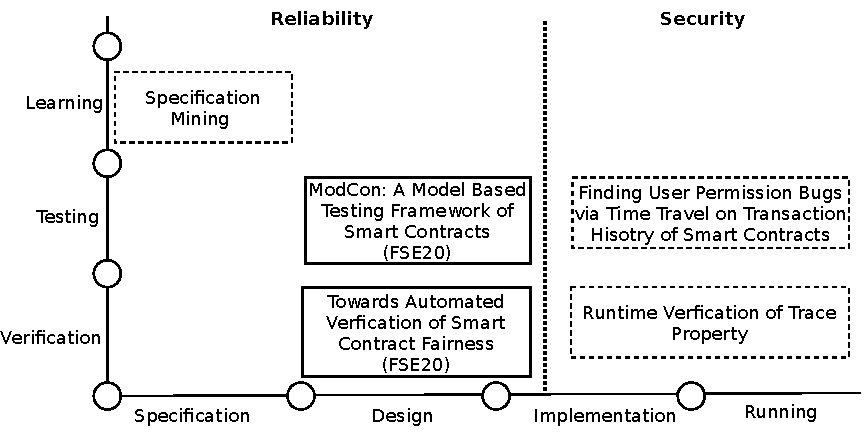
\includegraphics{./Figures/Chapter1/ThesisOverview}
	\caption{The overview of the current work (solid box) and future works (dashed box).}
	\label{fig: thesisoverview}
\end{figure}

To conclude, in this paper, our (future) research aims are threefold:
(1) Ensure smart contract security by performing model based testing for enterprise smart contracts. 
(2) Learn likely specification requirement of smart contracts via time travel on transaction history. 
(3) Verify smart contract fairness of smart contract that reflect the interactions between users and contract.


\section{Main Work and Contribution}
%Our research aims are twofold: (1) ensure smart contract security by performing model based testing for stateful enterprise smart contracts and DApp smart contracts rich in transactions. 
%(2) verify smart contract fairness by modeling users' interaction within smart contract.

\paragraph{Main Work and Contributions}
Our main works and contributions are summarized as follows.
%\yi{Spell out the contributions directly, not through questions.
%For example, what you have designed, proved, implemented, and evaluated.}
%\vspace{-.05in}
\begin{itemize}[leftmargin=*,topsep=4pt]
\item We proposed a general fairness verification framework, \faircon, to check fairness properties of smart contracts.
In particular, we demonstrated \faircon on two types of contracts and four types of fairness properties.
In addition to discovering property violations for bounded models, we apply formal
verification to prove satisfaction of properties for the unbounded cases as well.

\item We designed \modcon allowing users to provide a test model for smart contracts. 
The model is used to specify the state definitions, expected transition relations, pre/post conditions for each transition, invariants, and the mapping from the model to the contract code.
Given the test model, the testing process can also customized by choosing from different coverage strategies and test prioritization options.
\modcon then generates tests with the goal that exercise as many system behaviors as possible while prioritizing on cases of particular interests.

%\item  We proposed a novel approach to apply history transactions for reverse engineering access control models of smart contract. 
%We extracted role-based access control models from history transactions and studied and verified two types of access constraints: (1) separation of duty constraint, and (2) cardinality constraint.
\end{itemize}



\section{Organizations}
The rest of the thesis is organized as follows.
\Cref{ch:preliminary} presents the necessary background about smart contract and blockchain transaction.
The general fairness verification framework, \faircon, will be discussed in \Cref{ch:faircon}.
\Cref{ch:modcon} introduces \modcon, a model-based testing platforms of smart contract.
\Cref{ch:futurework} illustrates our future work, which aims to find permission bugs via time travel on transaction history of smart contracts,
and then this report will be concluded in \Cref{ch:conclusion}.

%\paragraph{Key Terms}
%Smart Contract; Model-based testing; Fairness verification; Program invariant; Automata learning.

%\paragraph{Tip}
%Literature Review; Contribution.
\chapter{Preliminary}
\chaptermark{Preliminary}
\label{ch:preliminary}
\begin{figure}[t]
	\centering
	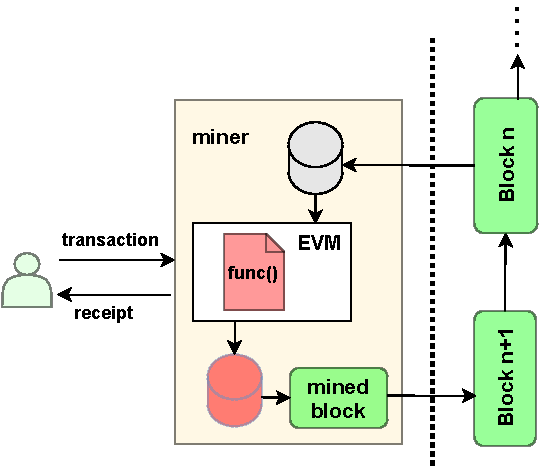
\includegraphics[scale=0.7]{Figures/Chapter5/SmartContractTransaction.pdf}
	\caption{The smart contract transaction on Ethereum.}
	\label{fig:smartcontractTransaction}
\end{figure}

A \emph{blockchain} is often called a distributed ledger recording transactions, consisting of blocks linked by cryptographic hashes and managed by a peer-to-peer network.
A blockchain can support not only transactions among users but also transactions between users and smart contracts.
\emph{Ethereum} is one of the most popular blockchains today, as it supports smart contracts~\cite{}.
A \emph{smart contract} is a piece of code that is executed autonomously on the blockchain; the execution of the code usually incurs a small fee, and a transaction executed by a smart contract may affect its own balance or the balance of another smart contract.
Figure~\ref{fig:smartcontractTransaction} briefly shows smart contract transaction on Ethereum.
A user (or client) sends a transaction to a miner for executing a specific contract function after block $n$.
The miner then reads the blockchain state database and runs on it the called function whose operation codes are interpreted by Ethereum virtual machine (EVM).
Later, the blockchain state database transitions and the miner will commit the new state database to a mined block that is appended as block $n+1$ after validation.
Finally, the user gets a receipt to confirm the transaction result including its status, event logs, ether transferred, as well as gas consumption.\footnote{Gas is the fee paid to the miner by transaction sender.}
If the transaction status indicates success, the state of contract will transition to new one. Otherwise, the contract state will remain unchanged.
\begin{definition}
	\textbf{Contract State and Transaction.} 
	A contract state $\delta$ can be defined by $<\mathit{Bal}, G\_\mathit{vars}>$ where $\mathit{Bal}\in N$ is the cryptocurrency balance owned by the contract, and $G\_\mathit{vars}$ comprises the values of all the storage variables managed by the contract.
	For simplicity, we define a transaction to smart contract as $t\leftarrow <\mathit{sender}, \mathit{value}, \mathit{func}, \mathit{status}>$, where $\mathit{sender}$ is an external account to invoke the contract's function $\mathit{func}$, and $\mathit{value}$ is the amount of attached ether correspondingly. 
	If the function invocation succeeds, $\mathit{status}$ is ``1''; otherwise, $\mathit{status}$ is ``0''. 
	Hereby, the transition types of a contract state can be formalized as (a) and (b).
	\begin{align*}
		(a)\quad\delta \xrightarrow[t.\mathit{status}=0]{t} \delta \quad \quad
		(b)\quad\delta \xrightarrow[t.\mathit{status}=1]{t} \delta^{'}
	\end{align*}
	In this paper, we focus on the transitions of type $(b)$ as the state of a smart contract is changed by them.
\end{definition}

\begin{definition}
	\label{def: contractmodel}
	\textbf{Contract Model.} 
	A contract model $\mathit{M}$ can be defined by $(\delta_0, F, \Delta, T)$ where $\delta_0 \in \Delta$ is initial state of contract, $f \in  F$ is a public function of contract and $T \subseteq \Delta \times F \times \Delta $ is transition function of contract state.
	As stated before, only successful function invocation can change contract state.
	Further, the reachability of function is decided by predicates over current contract state instead of its input. 
	For simplicity, every function can be implied by a boolean program: $f\implies Precondition(\Delta_1) \land StateChanges(\Delta_2)$,  where \textit{Precondition($\Delta_1$)} is a set of predicates related to check of global variables, i.e., state variables of contract and \textit{StateChanges($\Delta_2$)} is a set of assignments of global variables.
\end{definition}

Meanwhile, most smart contracts are designed as an organization for a social purpose, where users explicitly or implicitly play different roles 
when they participate in smart contract via transactions.
These smart contracts have been widely adopted in many areas including finance, gambling, exchanges, governance, property and etc..
For instance, the Ethereum Name Service (ENS) uses contracts to provide the auction service for users bidding the domains on Ethereum;
Dicether uses contracts to maintain houses for users' participation in gambling games;
while CryptoKitties uses contracts to organize blockchain stores for the exchange, breeding and siring of digital pets implemented as non-fungible tokens (NFTs). 
Therefore, it is critical to ensure smart contracts achieve the safety for the sake of the security of managed digital assets belong to users of different roles.
%!TEX root=../mythesis.tex
% Chapter Template

\chapter{Toward Automated Verification of Smart Contract Fairness} % Main chapter title
\chaptermark{FairCon: Toward Automated Verification of Smart Contract Fairness}  % replace the chapter name with its abbreviated form
\label{ch:faircon} 
% Change X to a consecutive number; for referencing this chapter elsewhere, use \ref{ChapterX}

\section{Introduction}\label{Sec_Introduction}
The blockchain technology has been developed rapidly in recent years, since the introduction of
Bitcoin~\cite{nakamoto2008bitcoin} by Nakamoto in 2008.
The distributed and tamper-resistant nature of blockchain has made it the perfect platform for
hosting smart contracts.
%Nowadays, blockchain technology has been widely applied to support many critical complicated
%systems by resorting to Turing-complete smart contract, thus there are a lot of booming
%applications beyond cryptocurrencies, which have not yet to be studied very well.
Smart contracts are computer programs running atop blockchain platforms to manage large sums of
money, carry out transactions of assets, and govern the transfer of digital rights between multiple
parties.
Ethereum~\cite{Ethereum} and EOS~\cite{EOS} are among the most popular blockchain platforms which
support smart contracts and have them applied in many areas.
%Among those platforms, Ethereum is considered one of the most promising where millions of smart
%contracts are running on.
%These smart contracts have shown their enormous capability to apply to diverse fields such as
%electronic auction and computer games, where centralized software platforms have not worked very
%well.
%It also has its unique advantage beyond past technology, especially for some other unexpected
%domains such as the token economy.
As of February 2020, there are over one million smart contracts deployed on Ethereum, which is a 100
fold increase since just two years ago.
These smart contracts have enabled about 2.7K decentralized applications (DApps)~\cite{dapp-stats}
serving 20K daily users on finance, health, governance, gambling, games, etc.
%As we know, in 2019, Moscow adopted smart contract technology in its parliament election
%\cite{election_attacks}.
%However, according to Gaudry reports \cite{gaudry2019breaking}, we know
%that this voting system is not perfect since it is said to be at the risk of encryption leakage.
%We also know that for EOS platforms, attacks to the game have caused faithful players suffering a
%lot, such as Dice, EOS attacks~\cite{EOS_attacks}.
%For the Ethereum platform, the DAO attack~\cite{DAO_attacks} is the most famous security event
%which brings the loss of \$60,000,000 worth, where the attacker exploited the reentrancy
%vulnerability underlying the DAO contract. T
%he smart contract, as a booming technology, is inclined to high chance of being attacked because
%of its immaturity in its characteristics and poor development quality by non-expert developers.

%Therefore with the increasing impact of security events in the smart contract, there are a
%considerable number of researches focus on these security problems. Oyente
%\cite{oyente,luu2016making} deserved high acknowledgment to first present a wide existence of some
%of the mentioned vulnerabilities in the smart contract on a large scale. Atzei et al.
%\cite{atzei2016survey} surveyed and analyzed large amounts of existing attack reports to offer a
%relatively comprehensive taxonomy of vulnerabilities based on different occurring contexts and
%characteristics. At the same time, some researches focus on the detection of malicious smart
%contracts \cite{bhargavan2016formal, grishchenko2018semantic, hirai2016formal,
%hildenbrandt2017kevm, park2018formal}. However, all of them have not considered the properties of
%smart contract beyond the security, which is the fairness property of smart
%contract.

%\begin{comment}
%\yi{This paragraph seems not so directly related. maybe put it in related work. better to focus on
%fairness in the intro: what are the different fairness considerations/properties?}
%Therefore with the increasing impact of security events in smart contract, there is a considerable
%number of researches focus on these security problems, which we can divide into two perspectives.
%One is to migrate traditional program security domain knowledge to the smart
%contract.
%Survey have presented possible bug types in smart contract including common integer overflow, owing
%to which Meitu Coin had been ruined, exception disorder that in essence seems likely to resemble
%exception handling in Java and other programming language. Lots of tools have been created to
%explore these bugs or to avoid these vulnerabilities. Among of which, Oyente
%\cite{oyente,luu2016making} deserved high acknowledgment to first present widely existence of some
%of the mentioned vulnerabilities in smart contract at large scale. The other one could be the
%research coupled with the application domain of
%smart contract. Of the different application domains, ERC token has been studied by many researches.
%[]  Token specification, [] Token event order consistency, [] token behaviors. However, all of
%them have not considered the properties of the smart contract after the security guaranteed, which
%is we focus on the
%fairness properties of the smart contract.
%\end{comment}

The security of smart contracts has been at the center of attention, ever since their adoption in
the management of massive monetary transactions.
One of the most notorious cases is the DAO attack~\cite{DAO_attacks} on Ethereum, which resulted in
a loss of \$60 million worth, due to the \emph{reentrancy vulnerability} being exploited by
malicious attackers.
Several gambling games on EOS, including \texttt{EOS.WIN} and \texttt{EOSPlay}, were recently
hacked using a technique called the \emph{transaction congestion attack}~\cite{EOS_attacks} and led
to significant asset loss.
What these incidents share in common is that certain security vulnerabilities neglected during
contract development are exploited by malicious parties, causing a loss for the contract owners
(and possibly other honest participants).
These vulnerabilities are programming errors, indicating a mismatch between the contract
developers' expectations and how the contract code actually works.
They are easy to detect once the vulnerability patterns are recognized.
In fact, much research has been dedicated to preventing, discovering, and mitigating such attacks.

In contrast, the \emph{fairness} issues of smart contracts have not yet attracted much attention.
A smart contract is unfair to certain participants if there is a mismatch between the participants'
expectations and the actual implementation of the game rules.
It is possible that a malicious party may gain an advantage over others through the exploitation of
security vulnerabilities, e.g., examining other participants' actions in a sealed game.
In this paper, we would like to focus more on the fairness issues introduced by the logical design
of the contracts instead, which are orthogonal to the security issues.
For example, smart contracts may well be advertised as ``social games'' with a promised 20\% return
for any investment, but turn out to be ``Ponzi schemes''~\cite{BARTOLETTI2020259}.
In this case, the possibility that the game may eventually slow down and never pay back is
intentionally left out.
Similarly, many auction DApps claim to be safe and fair, yet it is still possible for bidders to
collude among themselves or with the auctioneer to make a profit at the expenses of the
others~\cite{wu2018cream}.
The fairness issues mostly reside in contract logic: some of them are unfair by design, while the
rest are careless mistakes.
This makes the detection of such issues particularly challenging, because every case can be
different and there is no hope in identifying predefined patterns.
Since it is often not the contract creators' interest at risk (or even worse when they gain at the
expenses of participants), there is little incentive for them to allocate resources in ensuring the
fairness of their contracts.
On the other hand, it is rather difficult, for inexperienced users, to tell whether a contract works
as advertised, even with the source code available.

%The fairness problem exists even though security of smart contract are assured.
%Specifically, mechanism design is to study how to allocate resource to different participants.
%However, the mechanism design behind smart contract can be biased and the contract may be
%beneficial to several users, meanwhile other users will suffer loss.
%Because this problem should be ascribed
%to how well the mechanism design is for the smart contract. Unfortunately, the mechanism-related
%fairness property
%can not be tested or verified using existing work. Due to smart contract steadily extending its
%use in more critical domains such
%as auction and voting system and etc., understanding mechanism design could help relieve the
%fairness problems that smart contract will
%be confronted with.

%For smart contract, its mechanism design largely seems to be transparent to the participants.it
%might still be challenging for normal participants to understand the obscure syntax and subtle
%semantic implications of the contract source code.
In this paper, we present \faircon, a framework for verifying fairness properties of smart contracts.
Since general fairness is largely a subjective concept determined by personal preferences, there is
no universal truth when considering only a single participant.
We view a smart contract as a game (or mechanism~\cite{jackson2014mechanism,nisan2001algorithmic}),
which accepts inputs from multiple participants, and after a period of time decides the outcome
according to some predefined rules.
Upon game ending, each participant receives certain utility depending on the game outcome.
With such a mechanism model, we can then verify a wide range of well-studied fairness properties,
including \emph{truthfulness}, \emph{efficiency}, \emph{optimality}, and \emph{collusion-freeness}.
It is also possible to define customized properties based on specific needs.

The real challenge in building the fairness verification framework is on how to translate arbitrary
smart contract code into standard mechanism models.
Our solution to this is to have an intermediate representation for each type of games, which has
direct semantic translation to the underlying mechanism model.
For instance, the key components in an auction are defined by the set of bidders, their bids, and
the allocation and clear price rules of the goods in sale.
To synthesize the intermediate mechanism model for an auction smart contract, we first manually
instrument the contract code with customized labels highlighting the relevant components.
Then we perform automated \emph{symbolic execution}~\cite{king1976symbolic} on the instrumented
contract to obtain symbolic representations for auction outcomes in terms of the actions from a
bounded number of bidders.
This is finally mapped to standard mechanism models where fairness properties can be checked.
We either find property violations with concrete counterexamples or are able to show satisfaction
within the bounded model.
For properties of which we do not find violation, we attempt to prove them for unbounded number of
participants on the original contract code, with program invariants observed from the bounded cases.

%We aim to create a trustworthy faircon for smart contract participants to
%let them know whether the mechanism behind this contract is fair.
%Our approach is based on the
%mechanism design theory \cite{jackson2014mechanism,nisan2001algorithmic},
%facilitating symbolic
%execution to verify fairness properties related to mechanism from the smart contract. The key
%challenges for our approach can be divided into two aspects: One is to formally present a semantic
%framework for the mechanism model, where we can accurately define the fairness property based on
%the mechanism design. Another challenge is how to map the smart contract into the mechanism model.
%To better illustrate the method to solve them, we use an auction example to illustrate how to do.
%Our basic method is to define auction domain abstract syntax and its inductive rules from the
%abstract syntax to the mechanism model, rather than translate original smart contract into the
%mechanism model directly.
By introducing the intermediate representations, we could keep the underlying mechanism model and
property checking engine stable.
We defined an intermediate language for two types of game-like contracts popular on Ethereum, i.e.,
auction and voting.
We implemented \faircon to work on Ethereum smart contracts and applied it on 17 real auction and
voting contracts from \texttt{Etherscan}~\cite{Etherscan}.
The effort of manual labeling is reasonably low, considering the structural similarity of such
contracts.
The experimental results show that there are many smart contracts violating fairness property and \faircon is effective to verify fairness property and meanwhile achieves relatively high efficiency.


%\begin{comment}
%Actually, there are some existing works that focus on the fairness problem. Kalra et al.
%\cite{kalra2018zeus} first presented a framework named \textit{ZEUS} to verify the correctness and
%validate the fairness of smart contracts. However, the fairness problem they considered is only
%for
%the coding logic correctness, rather than the whole mechanism design fairness. Wu et al.
%\cite{wu2018cream} seem to be the first to consider the mechanism design problem of the smart
%contract. But they only designed a collusion-resistant k-Vickery auction implemented in the smart
%contract, rather than the fairness detection faircon in our work. Because even though the game rules
%are meant to be transparent, which is promised by the design of smart contracts, it might still be
%challenging for normal participants to understand the obscure syntax and subtle semantic
%implications of the contract source code. We should design a faircon to tell users whether this smart
%contract is fair for them.
%\end{comment}
%\begin{comment}
%\yi{Two things got mixed up here: (1) important applications where fairness is important and must
%be enforced to protect the participants; (2) the possible solutions including previous work, which
%have certain limitations motivating our work. These two should be put in separate paragraphs.}
%With smart contract steadily extending its use in more critical domain such as auction, vote
%system, classic mechanism design problems are also arising in smart contract and lack of design
%evaluation faircon makes these problems prone in smart contract. Inspired by Quantitative Analysis of
%Smart contract, Author use game theoretical model to study the mathematics of smart contract. To
%some extent, mechanism design can be seen as reverse game. Thanks to CREAM’s research on mechanism
%design for realizing a collusion-resistant smart contract auction, we observed well designed
%mechanisms as backbone of auction smart contract. For auction, general mechanism could be and its
%problems could be , For voting, general mechanism could be and its problems could be
%\end{comment}

\paragraph{Contributions}
Our main contributions are summarized as follows.
%\yi{Spell out the contributions directly, not through questions.
%For example, what you have designed, proved, implemented, and evaluated.}
%\vspace{-.05in}
\begin{itemize}[leftmargin=*,topsep=4pt]
	\item We proposed a general fairness verification framework, \faircon, to check fairness properties of
	smart contracts.
	In particular, we demonstrated \faircon on two types of contracts and four types of fairness
	properties.
	\item We defined intermediate representations for auction and voting contracts, and designed a
	(semi-)automated approach to translate contract source code into mathematical mechanism models
	which enable fairness property checking.
	\item In addition to discovering property violations for bounded models, we apply formal
	verification to prove satisfaction of properties for the unbounded cases as well.
	\item We implemented \faircon and evaluated it on 17 real-world Ethereum smart contracts.
	The results show that \faircon is able to effectively detect fairness violations and prove fairness
	properties for common types of game-like contracts.
	%  most auction contracts have fairness issues. Among 12 auction
	%  contract, 8 contracts were found unfair and 4 auction contracts are fair on one to three
	%fairness
	%  properties.
	The dataset, raw results, and prototype used are available online:
	\url{https://doi.org/10.21979/N9/0BEVRT}.
\end{itemize}

\paragraph{Organizations}
The rest of the paper is organized as follows.
\Cref{Sec_MotivatingExample} illustrates the workflow of \faircon with an example.
\Cref{section:mechanism_property} presents a general mechanism analysis model and defines a
modeling language customized for auction and voting contracts, serving as an intermediate
representation between the contract source code and the underlying mechanism model.
We then describe the model construction and fairness checking as well as verification techniques in
\cref{Sec_Method}.
\Cref{Sec_Evaluation} gives details on the implementation and presents the evaluation results.
\Cref{Sec_RelatedWorks,Sec_Conclusion} compare \faircon with the related work and
conclude the paper, respectively.



\section{\faircon by Example}\label{Sec_MotivatingExample}

%Because the smart contract can be viewed as a trusted third-party program to perform the trusted
%auctioneer, e-auction smart contracts have been more and more prevalent. As we know, the auction
%in
%the smart contract has been becoming a prominent part of Ethereum. So

In this section, we use an auction contract to illustrate how our approach works in
constructing the intermediate mechanism model and verifying fairness properties.

\begin{example}\label{exp:cryptorome}
	\Cref{CryptoRomeAuction} shows a simplified Ethereum smart contract,
	named \texttt{CryptoRomeAuction}, written in Solidity~\cite{solidity}, taken from
	\texttt{Etherscan}.\footnote{\url{https://etherscan.io/address/0x760898e1e75dd7752db30bafa92d5f7d9e329a81}}
	The contract implements a variant of open English auction for a blockchain-based strategy game,
	where players are allowed to buy virtual lands with cryptocurrencies.
	The auction is given a predefined life cycle parameterized by start and end times.
	A participant can place a bid by sending a message to this contract indicating the value of the bid.
	The address of the participant and the bid amount are stored in variables \texttt{msg.sender} and
	\texttt{msg.value}, respectively.
	The address of the current highest bidder is recorded in \texttt{highestBidder} (Line 9), and a
	mapping \texttt{refunds} is used to keep the contributions of each participant (Line 10) for
	possible refunding later.
	The \texttt{bid()} function (Lines 11--21) is triggered upon receiving the message.
	The bid is rejected if the bid amount is no more than the sum of the current highest bid
	and the minimal increment value \texttt{duration} (Lines 13--15).
	Otherwise, the previous \texttt{highestBidder} gets a refund (Lines 16--18), and the
	\texttt{highestBidder} (Line 19) and \texttt{highestBid} (Line 20) are updated accordingly.
\end{example}

\begin{figure}[t]
	\centering
	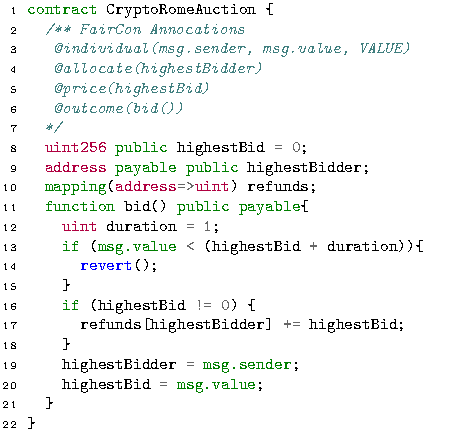
\includegraphics[width=.9\columnwidth]{Figures/Chapter2/auction.pdf}
	\caption{The CryptoRomeAuction Solidity source code.}\label{CryptoRomeAuction}
\end{figure}


%\begin{comment}
%\begin{figure}[t]
%  \small
%  \begin{align*}
%    & \texttt{CryptoRomeAuction} := (msgsender_1, msgvalue_1, \_ ) \\
%    & \quad (msgsender_2, msgvalue_2, \_ ) \\
%    & \quad (msgsender_3, msgvalue_3, \_ ) \\
%    & \quad (msgsender_4, msgvalue_4, \_ ) \\
%    & \quad (msgsender_5, msgvalue_5, \_ ) \\
%    & \quad \texttt{\textbf{assume}}:\; (\mnot (msgvalue_2 < msgvalue_1 + 1)) \mand \\
%    & \quad\quad (\mnot (msgvalue_3 < msgvalue_2 + 1)) \mand \\
%    & \quad\quad (\mnot (msgvalue_4 < msgvalue_3 + 1)) \\
%    & \quad \texttt{\textbf{allocate}}:\; \texttt{\textbf{argmax}}(msgvalue_1,
%    msgvalue_2, msgvalue_3,\\
%    & \quad\quad msgvalue_4,msgvalue_5)\\
%    & \quad \texttt{\textbf{price}}:\; \texttt{\textbf{max}}(msgvalue_1, msgvalue_2,
%    msgvalue_3,\\
%    & \quad\quad msgvalue_4,msgvalue_5)
%\end{align*}%
%  \caption{The mechanism model of CryptoRomeAuction with five bidders.}\label{Crypto_Mechanism}
%\end{figure}
%\end{comment}
\paragraph{Threats to Contract Fairness}
One way that \texttt{CryptoRomeAuction} can become unfair to the participants is through the so
called \emph{shill bidding}~\cite{jenamani2007cheating}---a shill tries to escalate the price
without any intention of buying the item.
This can be induced by either the auctioneer or adversarial participants, and other bidders may
need to pay more as a result.
Occasionally, the shill wins the auction if no other higher bid comes before auction ends.
The item may then be sold again at a later time.

\begin{table}[t]
	\caption{Example instances of CryptoRomeAuction.}\label{tab:example}
	\centering\small
	\begin{tabular}{l|ccc|ccc|ccc}
		\toprule
		& \multicolumn{3}{c|}{Truthful} & \multicolumn{3}{c|}{Untruthful} &
		\multicolumn{3}{c}{Collusion} \\
		\midrule
		Bidder & $p_1$ & $p_2$ & $p_3$ & $p_1$ & $p_2$ & $p_3$ & $p_1$ & $p_2$ & $p_3$ \\
		\midrule
		Valuation  & 3 & 4 & 6 & 3 & 4 & 6 & 3 & 4 & 6\\
		Bid  & 3 & 4 & 6 & 3 & 4 & 5 & 3 & 0 & 4 \\
		Allocation  & \xmark & \xmark & \cmark & \xmark & \xmark & \cmark & \xmark & \xmark & \cmark \\
		Price & 0 & 0 & 6 &  0 & 0 & 5 & 0 & 0 & 4 \\
		Utility  & 0 & 0 & 0 & 0 &  0 & 1 & 0 & 1 & 1 \\
		\bottomrule
	\end{tabular}
\end{table}

Apart from shill bidding, there are a number of other well-studied properties from the game theory
and mechanism design literature, which can be used to evaluate the fairness of an auction.
We use the example instances shown in \cref{tab:example} to demonstrate.
Suppose there are three bidders, $p_1$, $p_2$, and $p_3$, participating in the auction.
Each of them has a valuation of the item, i.e., the item worth three, four, and six units of utility for
$p_1$, $p_2$, and $p_3$, respectively.
The Columns ``Truthful'', ``Untruthful'', and ``Collusion'' in \cref{tab:example} show the
three example scenarios, where the players act truthfully, untruthfully, and collude among
themselves.
The Rows ``Bid'', ``Allocation'', ``Price'', and ``Utility'' show the bids placed, the final
allocation of the item, the clear price, and the utilities obtained by the bidders, respectively.

Same as other first-price auction schemes, \texttt{CryptoRomeAuction} is not \emph{truthful}, i.e.,
bidding truthfully according to one's own valuation of the item is not a dominant strategy.
%Here we show a bidder can cheat in since $CryptoRomeAuction$ cannot have positive incentive to
%drive bidder to truthfully report his bid price.
%Consequently, that cheating bidder could make higher utility while the auction seller suffer the
%loss.
In the ideal truthful scenario, all bidders bid according to their valuations, and $p_3$ wins the
bid with a utility of zero, because the payment equals to his/her valuation of the item.
In another scenario, where $p_3$ bids five (untruthfully), his/her utility would increase by one because
of the lower clear price.
This is called \emph{bid shading}, which only affects the revenue from the auction in this example,
but may affect other participants' utilities in some other cases.
%Further, this cheating benefit may bring negative incentive to other bidders to exercise their
%own truthful bid for this auction as well, which could damage the social welfare realizing in the
%auction.

In the third scenario, $p_2$ and $p_3$ collude in order to gain extra profits.
With full knowledge of each other's valuations, $p_2$ and $p_3$ may decide to form a cartel and
perform bid shading.
One possibility is to have $p_2$ forfeit his/her chance and $p_3$ bids four, and they divide the
profit equally among themselves.
Each of them gains one unit of utility as a result.

%Similar to this example, we also had found cheating problem widely exists in smart contract even
%though there exist many well designed truthful mechanisms available. Unfortunately, many auction
%smart contract try to give a fair illusion to users either via having a promising name or via
%exaggerating its functionality, in order to attract more users involved in the smart contract.
%Meanwhile, the opacity of fairness property of smart contract might make potential users unwilling
%to participate in auction smart contract, thereby decreasing possible social welfare further. Upon
%knowing the fairness properties of auction or other similar type of smart contract,  user may make
%reasonable decision to participate or not in the smart contract.

\paragraph{Checking Fairness Properties}
%\yi{We need to talk about (high-level) how to check fairness properties, such as collusion, on this example automatically.}
Given a mechanism model abstracting the auction settings, the set of fairness properties are
well-defined and can be formally specified based on the model.
The main challenge remains on how to extract the underlying mechanism model from the smart contract
source code.
Now we illustrate how this is done for \texttt{CryptoRomeAuction} in \faircon and outline the process
of automated property checking as well as verification.

%An auction smart contract can be seen as one implementation of some mechanism. To evaluate whether
%auction contract enables truthful incentive or not, we should observe the input and outcome of
%auction related mechanism.
Albeit variations in implementations, all auction contracts share some common components, such as
the bidders' identifiers, their bids, and the allocation as well as clear price rules.
We rely on users to provide annotations for these components directly on the source code, which are
demonstrated on Lines 2--7 in \cref{CryptoRomeAuction}.
Specifically, the annotations specify the bidders' information as a tuple,
``\texttt{@individual(msg.sender,msg.value)}'', indicating the variables used to store the
identifier and the bid value, respectively.
Similarly, ``\texttt{@allocation(highestBidder)}'' and ``\texttt{@price(highestBid)}'' indicate
that the allocation result and the clear price are stored in \texttt{highestBidder} and
\texttt{highestBid}, respectively.
Finally, ``\texttt{@outcome}'' is used to label the function defining the auction allocation logic.

\begin{figure}[t]
	\small
	\begin{align*}
		& \texttt{CryptoRomeAuction} := (msgsender_1, msgvalue_1, \_ ) \\
		& \qquad (msgsender_2, msgvalue_2, \_ ) \\
		& \qquad (msgsender_3, msgvalue_3, \_ ) \\
		& \qquad \texttt{\textbf{assume}}:\; (\mnot (msgvalue_2 < msgvalue_1 + 1)) \mand \\
		& \qquad\qquad (\mnot (msgvalue_3 < msgvalue_2 + 1)) \\
		& \qquad \texttt{\textbf{allocate}}:\; \texttt{\textbf{argmax}}(msgvalue_1,
		msgvalue_2, msgvalue_3)\\
		& \qquad \texttt{\textbf{price}}:\; \texttt{\textbf{max}}(msgvalue_1, msgvalue_2,
		msgvalue_3)
	\end{align*}%
	\caption{The mechanism model of CryptoRomeAuction with three bidders.}\label{Crypto_Mechanism}
\end{figure}

With these labels, we perform symbolic execution~\cite{king1976symbolic} on the \texttt{bid()}
function treating the participants' inputs---\texttt{msg.value}---as \emph{symbolic variables}.
The result of this would be two symbolic expressions for both \texttt{highestBidder} and
\texttt{highestBid}, which symbolically represent the allocation and clear price functions,
respectively.
We can then use these information to synthesize an intermediate mechanism model, shown in
\cref{Crypto_Mechanism}.
The model is specified in a customized language designed for auction and voting contracts.
Details of the language syntax and semantics can be found in \cref{section:mechanism_property}.
At the high level, the model specifies information of the participating individuals and the auction
rules: we consider a bounded model with only three bidders (i.e., $msgsender_1$, $msgsender_2$, and
$msgsender_3$), their bids have to satisfy the constraint specified in the \texttt{assume} clause,
the allocation function is given as ``$\argmax(msgvalue_1,\allowbreak msgvalue_2,\allowbreak
msgvalue_3)$'', and the clear price function is given as ``$\max(msgvalue_1,\allowbreak
msgvalue_2,\allowbreak msgvalue_3)$''.


%In our example as shows in Table \ref{tab:example}, the bid price is the
%input while allocation and payment are parts of the outcome. However, we cannot rely on observing
%the simple input and outcome to reason the fairness property because the valuation of bidder is
%ignored when generating the outcome but useful when analyzing the outcome.
The intermediate mechanism model in \cref{Crypto_Mechanism} has well-defined mathematical
semantics, which can be used to check the desired fairness properties.
We encode both the model and the property with an SMT formula such that a counterexample exists if
and only if the formula is satisfiable.
More details on the encoding can be found in \cref{subsection:property_checking}.
If the formula is unsatisfiable, we are confident that the property holds for the bounded case with
three bidders.
We then attempt to prove the property by instrumenting the contract program with \emph{program
	invariants} encoding the allocation and clear price clauses synthesized previously, but
parameterized by an unbounded number of bidders.
The instrumented program and the property are then passed to a program verification faircon, such as
Dafny~\cite{dafny}, to perform the automated verification.

%Having the valuation in
%analyzing process, taking $CryptoRomeAuction$ as example, firstly we assume there are some players
%that successively update the current highest bidder, then next comes two situation: $M$ $M'$. M is
%ideally truthful for every bidder and we get the utility $u$ of last bidder, the winner in this
%scenario, $M'$ is truthful for every bidder but the last bidder,and we get the utility $u'$ of last
%bidder, also the winner in this scenario, Next comes the comparison between $u$ and $u'$. If $u'$
%is larger than $u$, we can conclude that the contract fails the truthfulness property.  Otherwise,
%we may have some confidence of the truthfulness property of the contract and need to verify it
%using invariant reduction that will discussed in Section \ref{Sec_Method}.











\section{The Analysis Framework for Smart Contract Fairness}
\label{section:mechanism_property}

%\textcolor{red}{Provide a general introduction and overview of the materials/methods and supply essential background information}

In this section, we first provide necessary background and definitions on mechanism models and
fairness properties well studied in the mechanism design
literature~\cite{jackson2014mechanism,nisan2001algorithmic}.
Then we give the abstract syntax and semantics of our mechanism modeling language to support
automated model construction and property checking.

\subsection{Smart Contracts as Mechanism Models}\label{sec:mechanism-model}
Mechanism design is used to design economic mechanisms or incentives to help attain the goals of
different stakeholders who participate in the designated activity.
The goals are mainly related to the outcome that could be described by participants' payoff and
their return in the activity.
We model the logic behind smart contracts with a mathematical object known as the mechanism.
%Largely because of many existing diverse definitions, here we formally describe the mechanism model
%for later understanding fairness property, without the loss of generality.

In a \emph{mechanism model}, we have a finite number of individuals, denoted by $N = \{1, 2, \ldots,
n\}$.
Each individual $i$ holds a piece of private information represented by a \emph{type}, denoted
$\theta_{i} \in \Theta_i$.
Let the types of all individuals be $\theta = (\theta_1, \ldots, \theta_n)$, and the space be
$\Theta = \times_i \Theta_i$.
The individuals report, possibly dishonestly, a \emph{type (strategy) profile} $\report \in \Theta$.
Based on everyone's report, the mechanism model decides an outcome which is specified by an
\emph{allocation function} $d: \Theta \mapsto O$, and a \emph{transfer function} $t: \Theta \mapsto
\mathbb{R}^n$, where $O = \{o_i \in \{0,1\}^n \mid \Sigma_i o_i = 1\}$ is the set of possible
outcomes.

The preferences of an individual over the outcomes are represented using a \emph{valuation function}
$v_i: O \times \Theta_i \mapsto \mathbb{R}$.
Thus, $v_i(o, \theta_i)$ denotes the benefit that individual $i$ of type $\theta_i$ receives from an
outcome $o \in O$, and $v_i(o,\theta_i) > v_i(o',\theta_i)$ indicates that individual $i$ prefers
$o$ to $o'$.
%Individuals may also need to make or receive payment, which is defined by a \emph{transfer
%function}
%$t_i: \Theta \mapsto \mathbb{R}$.
%\yi{TODO: some notations need to be fixed.}
%Having the benefit function $v$ over decisions and transfer
%function $t$, we can easily get the utility $u_i$ of the individual $i$: $ u_i(\theta) =
%v_i(d(\theta), \theta_i) - t_i(d(\theta), \theta_i^s)$. and the social welfare $W$ is sum of all
%individuals' utilities: $ W = \sum_{i=1}^n u_i(\theta)$.
The individual $i$'s utility under strategy profile \report is calculated by subtracting the
payment to be made from the valuation of a certain outcome: $u_i(\report) = v_i(\report,
\theta_i) - t_i(\report)$.

%A \emph{strategy} is a mapping from types to
%For simplicity, we also directly use $\theta_i^s$ to refer to individual's strategy to report his
%type.
%Generally, every individual has his own private information type independent of each other;
%We would use pair ($\theta_i$, $\hat{\theta_i}$) to represent the strategy to truthfully report
%individual's type and the strategy to untruthfully report individual's truthful type respectively,
%where $\theta_i \in \Theta_i$ and $\hat{\theta_i} \in \Theta_i$, $\Theta_i$ are the set of all
%strategies for individual $i$;

%Let $\theta = (\theta_1^s,\theta_2^s,\dots,\theta_n^s)$ be all individual's strategies, $\theta
%\in \Theta$ and
%$\theta_i^s \in \Theta_i$. Mechanism model takes as input individuals' strategies $\theta$ and as
%output an outcome $\Octon$ generated by a common social decision function $d(\theta)$ across
%individuals and a set of transfer function $t(d(\theta),\theta_i^s)$ for individual $i$. For
%social
%decision function $d(\theta) \in D$, where $D$ is the set of all possible social decisions made
%among the individuals. The transfer function $t(d(\theta),\theta_i)$ is to calculate, based on the
%decision $d(\theta)$ and $\theta_i$, the strategy of individual $i$, how much individual $i$
%should
%pay.

%\begin{definition}[Mechanism Model]
%A mechanism model $(N, \report, O)$ is described by a set of individuals $N$ and their input
%strategies $\theta$ and an outcome $\Octon$ subjects to a social decision function
%$d(\theta)$:$\Theta \rightarrow \N $ and a transfer function $t(d(\theta))$:$\Theta \rightarrow
%\R^n$. We denote as $t_i(d(\theta),\theta_i^s)$ the transfer for individual $i$.
%\end{definition}

%Furthermore, for any individual, which his strategy is would affect the decision afterwards and how
%much he should pay on that decision.
%So basically each individual has its preference over different social decisions.
%We use the benefit function $v_i(d(\theta), \theta_i)$ to denote the benefit value for the
%individual $i$ from the decision generated by $d(\theta)$.

\subsection{Fairness Properties}\label{subsec:FairnessProperty}
%\yi{Need to talk about why these properties.}
%\liu{ Fairness is a meaningful but broad problem of software development. Fairness itself seems to
%be generally subjected to different domains knowledge.}
%\liu{For most of the mechanism design practice, the need of a truthful-incentive mechanism ranks
%at the top,
%meanwhile keeping the mechanism efficient for user to participate and optimal for the mechanism
%stakeholders to benefit, the so-called maximizing the social welfare, also
%matter~\cite{jackson2014mechanism}.
%Moreover, a good mechanism design should resist against users' collusion~\cite{wu2018cream}.
%These needs or features construct mechanism fairness to some extent.
%}
The fairness of smart contracts is usually subject to the understandings and preferences of the
participating parties---a contract fair to someone may be unfair to the others.
In particular, fairness can be considered from both the participants' and the contract creators'
points of view.
To capture such nuances, individual parties have to be modeled separately before such subjective
fairness properties can be specified against the model.

Generally speaking, all properties which can be expressed in terms of the mechanism model defined
in \cref{sec:mechanism-model} are supported by our reasoning framework.
To keep the presentation simple, in this paper, we focus on analyzing a set of generic fairness
properties based on the mechanism models.
%\liu{The mechanism model itself can be used to model and verify fairness of any	game-like smart
%contract involving multiple participants.}
We restrict the discussion to four types of well-studied properties in the literature, namely,
truthfulness, optimality, efficiency, and collusion-freeness.

%\liu{These fairness properties matter a lot to smart contract. }
%\begin{comment}
%from 2-collusion mechanism to collusion-freeness fairness property, we may need a discussion to
%explain the gap. Because the gap acutally exists and matters.
%\end{comment}

To formally define the properties, we first introduce an important concept---\emph{dominant
	strategy}.
We use $\report_{-i}$ to denote the strategy profile of the individuals other than $i$, i.e.,
$(\report_1, \ldots, \report_{i-1},\allowbreak \report_{i+1},\allowbreak \ldots,\allowbreak
\report_n)$.
Therefore, $(\report_i', \report_{-i})$ is used to denote the strategy profile which differs from
\report only on $\report_i$.

\begin{definition}[Dominant Strategy]
	A strategy $\report_i \in \Theta_i$ is a dominant strategy for $i$, if $\forall
	\report_{-i} \forall \report_i' \in \Theta_i \cdot u_i(\report_i, \report_{-i}) \geq
	u_i(\report_i', \report_{-i})$.
	When equality holds, the strategy is a weak dominant strategy.
\end{definition}

We say that a mechanism model is truthful if and only if for any individual and strategy profile,
reporting one's real type (truth-telling, i.e., $\forall i \in N \cdot \report_i = \theta_i$) is a
dominant strategy.

\begin{definition}[Truthfulness]\label{def:truthful}
	Formally, a mechanism is truthful if and only if,  $\forall \theta_{-i} \forall \report_i \in
	\Theta_i \cdot u_i(\theta_{i}, \theta_{-i}) \geq u_i(\report_i, \theta_{-i})$.
\end{definition}
%<<<<<<< HEAD
%
%In an auction contract, the account which creates the auction is the \yi{beneficiary?} and the
%accounts which join the auction are the bidders.
%\yi{If the auction prevents bidders from gaining more by bidding less, it is said to be truthful.}
%Since bidding untruthfully is not a good strategy, truthful auctions can generally attract more
%honest participants so that the \yi{beneficiary?} can get much higher revenue for the item sold.
%=======
Given an auction smart contract with many bidders competing for a single indivisible good, the
account which creates the contract is the \emph{auctioneer} and the accounts which join the auction
are the \emph{bidders}.
If the auction prevents bidders from benefiting more by bidding less, it is truthful.
When bidding untruthfully is not a good strategy, the auction can generally attract more honest
bidders and the auctioneer can get higher revenue for the good on sale.


\begin{definition}[Efficiency]
	We say a mechanism is efficient if and only if its allocation function achieves maximum total
	value, i.e., $\forall \report \in \Theta \forall d' \cdot \sum_{i} v_{i}(d(\report), \theta_{i})
	\geq \sum_{i} v_{i}(d'(\report)$, $\theta_{i})$.
\end{definition}

Suppose no bidder can affect any other bidder's valuation.
If the only winner is the bidder who values the good the most, the auction is efficient.

\begin{definition}[Optimality]
	We say a mechanism is optimal if and only if its transfer function achieves maximum total net
	profit, i.e., $\forall \report \in \Theta \forall t' \cdot \sum_i t_i(\report) \geq
	\sum_i t_i'(\report)$.
\end{definition}

Similarly, if the winner is the one who bids the highest, the auction is optimal.
In this case, the auctioneer receives the highest revenue.

We use $\report_{-ij}$ to denote the strategy profile of individuals other than $i$ and $j$, i.e.,
$\{\report_1, \allowbreak \ldots, \allowbreak \report_{i-1}, \allowbreak \report_{i+1}, \ldots,
\report_{j-1}, \report_{j+1}, \allowbreak \dots, \report_n\}$.

\begin{definition}[2-Collusion Free]
	We say a mechanism is 2-collusion free if there does not exist a cartel of individuals $i$ and
	$j$, whose untruthful strategies increase the group utility, formally,
	$u_i(\hat{\theta_i}, \allowbreak \hat{\theta_j}, \allowbreak \theta_{-ij}) + u_j(\hat{\theta_i},
	\hat{\theta_j},\theta_{-ij}) \geq u_i(\theta_i, \allowbreak \theta_j, \allowbreak \theta_{-ij}) +
	u_j(\theta_i, \theta_j, \theta_{-ij})$.
\end{definition}
%<<<<<<< HEAD
%\liu{Above we present 2-Collusion free property.
%Briefly, if \texttt{Auction} can prevent any two bidders collusion by making their collusion gains
%not greater than their non-collusion gains, we say \texttt{Auction} is 2-collusion free, which
%could prevent bid price manipulation to some extent so as to realize higher revenue for its
%beneficer.}
%\yi{How about n-collusion free?}
%=======
Collusion is a big concern in auction and other multi-player games.
The basic 2-collusion freeness property in an auction means that any two bidders' collusion cannot
help them achieve higher gain.
This prevents bid price manipulation to a certain extent, which helps guarantee fair chance for all
bidders and maintain good revenue for the auctioneer.
A more general version, i.e., $n$-collusion freeness, can be defined in a similar way.
%>>>>>>> save fixes
%\lstset{numbers=none}
%Based on syntax given in Sect.~\ref{subsection:syntax}, we make some extension to the syntax and
%Fig.~\ref{syntax} draws the description language for the four fairness properties.

%\yi{Give intuitions about these definitions.}


\subsection{Mechanism Modeling Language}\label{subsection:syntax}

We now propose a domain-specific language to facilitate the automated translation from smart
contracts to mechanism models.


\begin{figure}[t]
	\small
	\begin{align*}
		\texttt{<individual>}  &:= (id: \mathbb{S}, bid: \N, val: \N ) \\
		\texttt{<func>}        &:= \texttt{\textbf{max}} \;|\; \texttt{\textbf{argmax}} \\
		\texttt{<exp>}         &:= \texttt{<individual>}.id \;\;|\;\; \texttt{<individual>}.bid \\
		&\;\;|\;\; \N \;\;|\;\; \texttt{<exp> \texttt{[+-]} <exp>}
		\;\;|\;\; \texttt{<func>(<exp>*)} \\
		\texttt{<bool>}        &:= \texttt{<exp> == <exp>} \;\;|\;\; \texttt{<exp> < <exp>} \\
		&\;\;|\;\; \mnot \texttt{<bool>} \;\;|\;\; \texttt{<bool>}
		\mand \texttt{<bool>} \\
		\texttt{<assumption>}  &:= \texttt{\textbf{assume}} : \texttt{<bool>} \\
		\texttt{<outcome>}     &:= \texttt{\textbf{allocate}} : \texttt{<exp>} \\
		&\;\;|\;\; \texttt{\textbf{price}} : \texttt{<exp>}; \;
		\texttt{\textbf{allocate}} : \texttt{<exp>} \\
		\texttt{<property>}    &:= \texttt{<bool>} \;\;|\;\; \texttt{\textbf{forall}} : \texttt{<bool>} \\
		\texttt{<mechanism>}   &:= \texttt{<individual>*}; \; \texttt{<assumption>}; \;
		\texttt{<outcome>}; \\
		&\quad\;\; \texttt{<property>}
	\end{align*}%
	\caption{Syntax of the auction/voting mechanism model.}\label{syntax}
\end{figure}

We define an abstract syntax of the mechanism modeling language, which is applicable to both auction
and voting.
\Cref{syntax} shows the context-free grammar of the language.
A mechanism model comprises one or more \emph{individuals}, an \emph{assumption}, an
\emph{outcome}, and a \emph{property} to be verified.
An individual is defined as a triple containing the identifier ``$id$'', bid amount ``$bid$'', and
valuation ``$val$''.
An assumption is a Boolean constraint which should be satisfied upon the entry of the contract.
The outcome of the contract is specified by the allocation and the clear price functions, which are
expressions over $id$ and $bid$.
Voting contract typically does not have a clear price function.
We allow properties to be specified using a Boolean expression optionally preceded by a ``forall''
quantifier.

\begin{figure}[t]
	\centering
	\AxiomC{$(id_1,bid_1,val_1), \ldots, (id_n,bid_n,val_n)$}
	\RightLabel{[Indiv]}
	\UnaryInfC{\stackanchor{$N \leftarrow \{1, \ldots ,n\}$ \quad $\report \leftarrow%
			\{bid_1,\ldots,bid_n\}$}%
		{$\{v_i(o_i, \theta_i)\} \leftarrow \{val_i\}$}}
	
	\DisplayProof \vskip .1in
	\AxiomC{$\texttt{\textbf{assume}}:assumption$}
	\AxiomC{$\texttt{\textbf{allocate}}:allocation$}
	\RightLabel{[Alloc]}
	\BinaryInfC{$d(\report) \leftarrow \textbf{eval}(assumption \wedge allocation)$}
	\DisplayProof \vskip .1in
	\AxiomC{$\texttt{\textbf{assume}}:assumption$}
	\AxiomC{$\texttt{\textbf{price}}:clearprice$ }
	\RightLabel{[Price]}
	\BinaryInfC{$t(\report) \leftarrow \textbf{eval}(assumption \wedge clearprice)$}
	\DisplayProof
	\caption{Semantic rules of the auction/voting model.}\label{semantics}
\end{figure}

\begin{figure*}[!t]
	\centering
	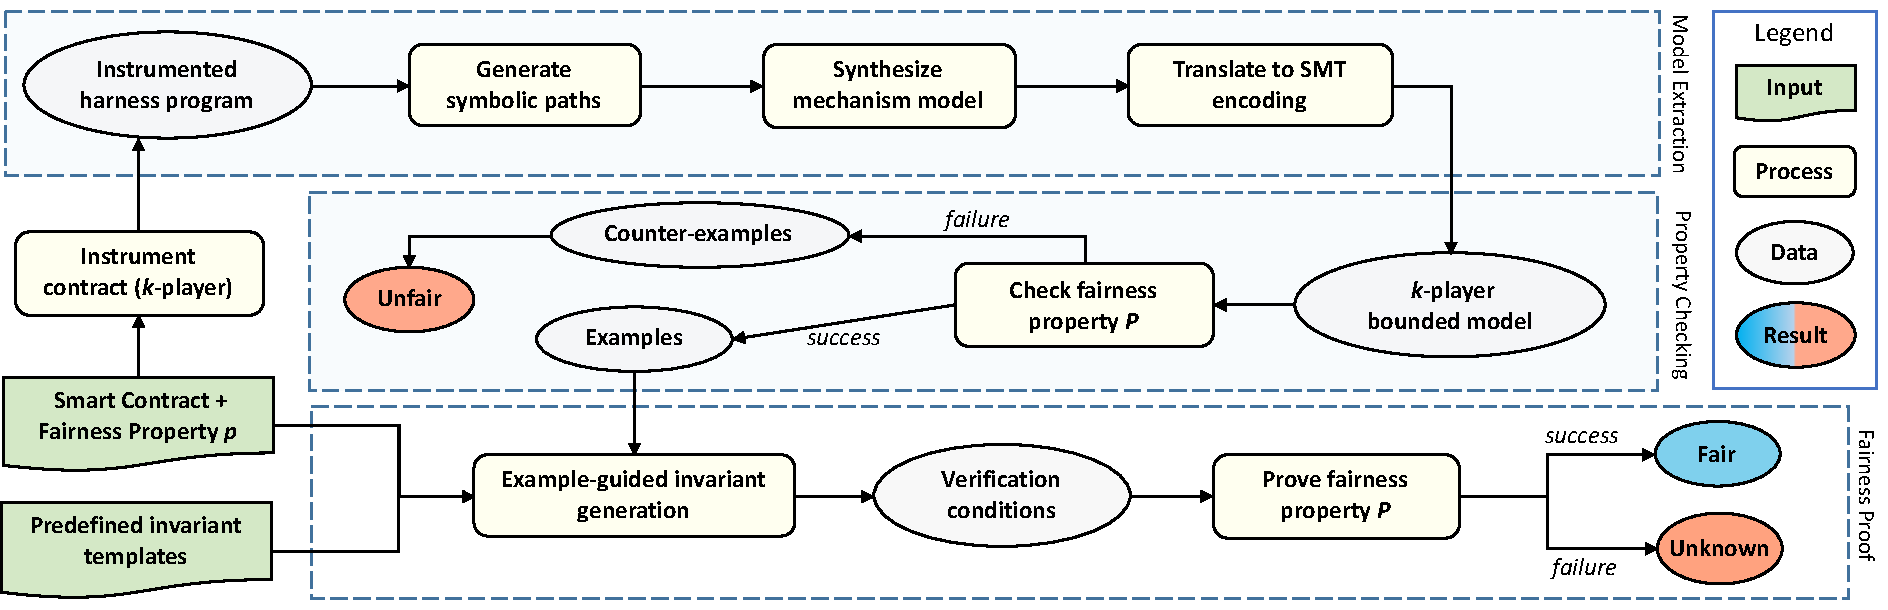
\includegraphics[width=\textwidth]{Figures/Chapter2/framework.pdf}
	\caption{Workflow of the \faircon framework.}\label{fig:framework}
\end{figure*}

\paragraph{Language Semantics}
The semantic mapping from the modeling language to the underlying mechanism model is summarized in
\cref{semantics}.
The ``Indiv'' rule maps the individuals and their reported types as well as valuations.
More specifically, the individuals' bids are mapped to their reported types \report, and an
individual of type $\theta_i$'s valuation of the item $v_i(o_i, \theta_i)$ is $val_i$, where $o_i$
denoted the outcome where the item is allocated to $i$.
The ``Alloc'' rule conjuncts the Boolean expression $assumption$ from the ``assume'' clause and the
symbolic expression $allocation$ in terms of individuals' strategies from the ``allocate'' clause,
which is evaluated as the allocation function.
Similarly, the transfer function is the conjunction of the $assumption$ and the $clearprice$
expressions.

There are some differences between auction and voting:
clear price is absent from voting, where allocation is done by comparing the number of ballots
(bids) by the participating individuals;
%Above we only present the outcome semantic rule for the auction.
whereas in auction, the individuals who bid no less than the clear price can be allocated the item.

This language works for the most commonly seen auction and voting contracts with fairness concerns.
For example, Ethereum smart contracts meeting the ERC-1202 (voting)~\cite{erc-1202} and ERC-1815
(blind auctions, under review)~\cite{erc-1815} standards all follow the same interface and
structure, therefore can be automatically translated into our modeling language.
Similar languages can also be designed for other types of contracts (e.g., social games).
The proposed modeling language can be modified and extended to establish suitable mappings from new contract types to the classic mechanism model.
With the new modeling language, the model extraction and property checking algorithms can be
directly reused.


\section{The \faircon Framework}\label{Sec_Method}
%\textcolor{red}{Restate the purpose of the work and provide specific and precise details about source of materials and methods}
%In the section 3, we have illustrated the mechanism model and also specified the
%four important fairness properties.

In this section, we present the \faircon verification framework for smart contract fairness.
\Cref{fig:framework} shows the overall workflow of \faircon.
The framework consists of three modules, namely, \emph{model extraction}, \emph{property checking},
and \emph{fairness verification}.

The smart contract source code is first automatically instrumented according to user-provided
annotations.
At this stage, we consider a $k$-player bounded model, and the instrumented contract code contains
a harness which orchestrates the interactions between the players and the target contract.
The extraction of the mechanism model is powered by symbolic execution of the harness program, and
an intermediate mechanism model is synthesized as a result.
%First one is symbolic execution of smart contract at source-code level, which is supported by the
%custom symbolic engine.

In order to perform property checking, the intermediate mechanism model, along with the desired
property, are encoded as an SMT formula, such that the formula is unsatisfiable if and only if the
property holds with respect to the model.
We use an SMT solver to check and may declare the property holds when the number of participants
are bounded by $k$; otherwise, a counterexample is generated which disputes the property.
%Next comes the property checking part, where our goal is to reveal some unfair
%smart contract by observing counterexample generated, which violates the fairness property.
%If the symbolic execution cannot generate counterexample, we manually use invariant-like technique
%to explore function scheme or say phase scheme related to mechanism design, to abstract smart
%contract, and then based on these abstract schemes, verify whether fair property holds or not
%without any misleading results.

If we fail to find a counterexample in the bounded case, we may proceed to the fairness
verification of the properties for unbounded number of participants.
To do that, we modify the harness to account for an unlimited number of players, instrument it with
program invariant as well as the desired properties as post-conditions, and rely on program
verification tools to discharge the proof obligations.
This either tells us that the property is successfully proved, or the validity of the property is
still unknown, in which case we are only confident about the fairness for the bounded case.


\subsection{Mechanism Model Extraction} \label{subsec:ModelExtraction}

\begin{figure}[t]
	\centering
	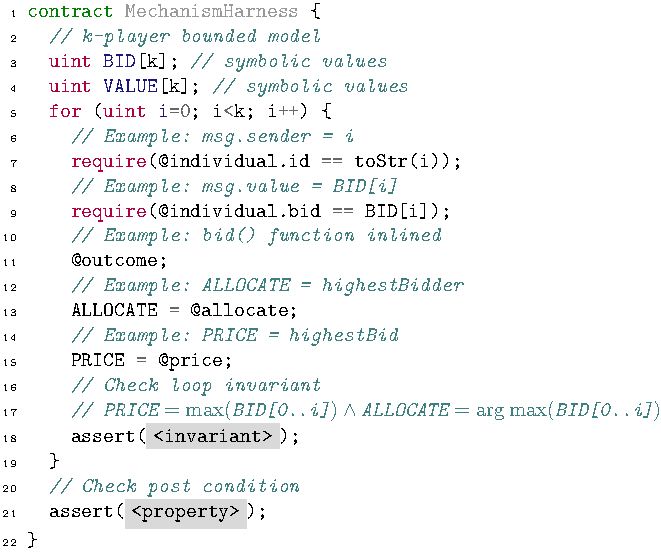
\includegraphics[width=\columnwidth]{Figures/Chapter2/harness.pdf}
	\caption{The harness program for mechanism model orchestration.}\label{fig:harness}
\end{figure}

%For smart contract, it has no limitation to the number of participants, since
%the smart contract has a dynamic mechanism model that could involve a lot of
%participants, which is difficult to manually analyze fairness properties on the
%smart contract. In most times, It is also difficult to analyze fairness property
%of complicated smart contract with even a small number of participants. So we
%propose a prototype faircon Solse+ to automatically check fairness properties on the
%smart contract. Our faircon can help: (1) developers to have an idea of fairness about
%their smart contracts from the perspective of the mechanism. (2) participants to
%be cautious to attend unfair smart contracts.

To extract a mechanism model out of the smart contract source code, we first instrument the
contract code with a harness program \texttt{MechanismHarness} shown in \cref{fig:harness}.
The harness program orchestrates the interactions of $k$ players with the target contract.
This is achieved by declaring symbolic variables to represent the possible bid and valuation of
each player, stored in the arrays ``\texttt{BID}'' (Line 3) and ``\texttt{VALUE}'' (Line 4),
respectively.
Then a for-loop (Lines 5--19) is used to simulate the actions performed by the $k$ players.
In smart contract, all players have to move sequentially since parallelization is not allowed.
The ordering is not important, because the players are symmetric.

We rely on the annotations provided by users (e.g., \cref{CryptoRomeAuction}) to construct the
loop body, which triggers a move from one particular player.
The variables controlling the player's identifier and bid value are assigned the corresponding
symbolic values (Lines 7 and 9).
In the case of \cref{exp:cryptorome}, these variables are \texttt{msg.sender} and
\texttt{msg.value}, respectively.
Then the allocation function (e.g., \texttt{bid()} in \cref{exp:cryptorome}) is inlined, and
the resulting variables annotated by \texttt{@allocate} and \texttt{@price} are stored as symbolic
expressions (Lines 13 and 15).
There are also two placeholders at Lines 18 and 21, for assertions of loop invariant and post
conditions, which will be described in \cref{subsection:formal_proof}.

We then run symbolic execution on the harness program to collect a set of feasible symbolic paths.
Each symbolic path is represented in the form of ``$\mathit{Condition} \wedge \mathit{Effect}$'',
where ``$\mathit{Condition}$'' and ``$\mathit{Effect}$'' are Boolean expressions in terms of the
symbolic variables defined earlier (e.g., \texttt{BID[i]} and \texttt{VALUE[i]} in
\cref{fig:harness}).
Here, ``$\mathit{Condition}$'' represents the \emph{path condition} which enables the execution of a
particular program path; ``$\mathit{Effect}$'' represents the values of the resulting variables
(e.g., \texttt{ALLOCATE} and \texttt{PRICE} in \cref{fig:harness}).
We take all path conditions $\mathit{Condition}_j$, where the effect is successfully computed
(i.e., not running into errors or reverts), and use the disjunction of them as the
$\mathit{assumption}$ of the model (i.e., ``\texttt{assume} $\bigvee_j \mathit{Condition}_j$'').
Similarly, we use the effects as the corresponding allocation and clear price functions.
For example, in the mechanism model, we have ``\texttt{allocate} $\bigvee_j (Condition_j \wedge
\mathit{Effect}_j[ALLOCATE])$'' and ``\texttt{price} $\bigvee_j (\mathit{Condition}_j \wedge
\mathit{Effect}_j[PRICE])$''.

%Our faircon Solse+ can check all possible collected symbolic paths.
%If there is checking failure on one path, the Solse+ will generate relevant counterexample for this
%path.
%The counterexample could also be deemed as an instance of the mechanism model of the smart contract
%in our context.
%
%We also have an extension integrated with our faircon to support the analysis of the mechanism model.
%This extension covers the variable notation function of the participants or so-called individuals.
%So Solse+ not only collects a symbolic path of smart contract but also collected the mechanism
%components and related fairness property expression.
%For simplicity, Solse+ first removes the unreachable paths


\subsection{Bounded Property Checking}\label{subsection:property_checking}
%\begin{comment}
%\textcolor{red}{Formal representation to fairness property checking problem}
%\begin{itemize}
%    \item  model formalization using formal notation
%    \item  different validity of property on mechanism model
%    \item  technical challenge
%    \item  taking mentioned example to illustrate how to check
%\end{itemize}
%\textcolor{red}{Fairness property analysis}
%\begin{itemize}
%    \item  present simple ground truth where mechanism is untruthful
%    \item  present simple ground truth where mechanism is truthful
%\end{itemize}
%\end{comment}
%Once our faircon recovers the mechanism model out of the smart contract, we can get the boolean
%expression of fairness properties and then check whether this expression can attain true value.
%Here we simply formalize the checking process for our fairness properties.

For property checking, given a mechanism model $M$ and a property $p$, our goal is to construct a
formula $\phi$ such that $\phi$ is unsatisfiable if and only if $M \models p$.
With the semantic rules defined in \cref{subsection:syntax}, it is straightforward to obtain a
formula encoding the allocation and clear price functions, i.e., $\varphi_M = d(\theta) \wedge
t(\theta)$.

We illustrate the encoding of properties using the truthfulness as an example.
\Cref{def:truthful} states that a model $M$ is truthful if and only if the truth-telling
strategy performs no worse than any other strategies.
Therefore, the high-level idea is to first encode the truthful and untruthful strategies separately
for an arbitrary player, and then asserting that the utility of the player is higher when he/she
acts untruthfully.
The encoding of the truthfulness property $p$ is shown as follows,%
\begin{align*}
	\exists i \cdot & \forall j \cdot (i \neq j) \implies \\
	& (\varphi_M \land (bid_i = val_i) \land (bid_j = val_j)) \tag{Truthful} \\
	\land\; & (\varphi_M[bid_i/bid_i', u_i/u_i'] \land (bid_i' \neq val_i)) \tag{Untruthful} \\
	\land\; & (u_i < u_i'), \tag{Utility}
\end{align*}%
where $i$ is a generic player with utility $u_i$.
The truthful scenario is when all players (including $i$) bid the same amount as their valuations,
i.e., $bid_i = val_i$ and $bid_j = val_j$.
The untruthful model is constructed by substituting the bid and utility variables of $i$ with new
copies $bid_i'$ and $u_i'$, and asserting $bid_i' \neq val_i$.
Finally, we assert that $u_i < u_i'$.
If $p$ is satisfiable, we find a counterexample where an untruthful strategy performs better than
the truthful strategy.
Otherwise, the truthful strategy is a dominant strategy for $i$.
The encodings of other properties are similar.
%Using the abstract syntax of a mechanism model, we could can denote a mechanism model using the
%notation $\phi: \{I, O\}$,
%where $I(x)$ refers to the individuals related information of a mechanism model,
%and $O(I(x))$ refers to the outcome of the mechanism given $I(x)$. Let  $\varphi$ be the fairness
%property, we can describe a particular property $\varphi$ of a given mechanism model $\phi$.
%$\phi$ could be simplified as $ \phi = O(\forall x I(x))$.

%We say a property $\varphi$ holds for a given mechanism model $\phi$ iff $ \varphi(\phi)
%\rightarrow \nexists O'\forall x \varphi(O'(I(x)))$ or $ \varphi(\phi) \rightarrow \forall x
%\varphi(O(I(x)))
%$. This means a property holds for a given model no matter what the participants are or its
%outcome function could be improved.

%In the paper, we explore whether the fairness property holds for mechanism model. Due to the
%difficulty of directly checking fairness property
%using symbolic execution on infinite formula, we compromised and checked whether a fairness
%property $\varphi$ holds for a given mechanism model
%under the setting of fixed number of participants.  We say a property $\varphi$ holds for a given
%mechanism model $\phi$ and $k$, the number of $I$ as $\varphi(\phi[\|I\|=k])$. And $
%\varphi(\phi[\|I\|=k])  \Leftrightarrow \nexists O' \forall x \varphi(O(I(x))) \lor \forall x
%\varphi(O(I(x)))$.Obviously, if we found $k$ that make
%property checking fail, we say the mechanism model is not fair w.r.t $\varphi$. On the contrary, we
%say the mechanism model is fair w.r.t $\varphi$ and $k$.
%Subsection \ref{subsection:formal_proof} will illustrate how to prove whether the k-fair mechanism
%model remain fair independent of $k$.
% \begin{figure}[!h]
%   \includegraphics[width=0.45\textwidth]{./figures/MethodTruthfulCheck}
%   \caption{The overview of fairness Property Checking}
%  \end{figure}

%We take truthful property as an example to illustrate our work.
%Assuming a bidder intends to make more profit by cheating on his bid value. This means his actual
%bid value $\hat{\theta}$ will be different from his truthful bid value $\theta$.
%We denote his utility as $u$ and have the following formulas. $ \textMu (\theta) \reduce u_0 $,
%$\textMu (\hat{\theta}) \reduce u_1 $. Truthful property could be expressed as below.
%\[
%    truthful = \begin{cases}
%         False,   & \text{if } u_1 > u_0\\
%         True,     & \text{otherwise}
%    \end{cases}
%\]
%And recall the example $CryptoRomeAuction$ mentioned in Section \ref{section:example}. There are 5
%bidders in the example. Assuming all $5$ bidders'
%value are $\theta_1$, $\theta_2$, $\theta_3$, $\theta_4$, $\theta_5$, only the first bidder intends
%to
%make more profit, so the first bidder would choose the untruthful value $\hat{\theta_1}$. So for
%the first bidder, his utility $u_1$ is as
%\[
%    u_1 = \begin{cases}
%        \theta_1 - \hat{\theta_1},   & \text{if }
%\hat{\theta_1}>max(\theta_2,\theta_3,\theta_4,\theta_5)+duration \\
%         0,     & \text{otherwise}
%    \end{cases}
%\]
%Similarly, if he choose to be truthful, his benefit $u_0$ could be as
%\[ u_0 = \begin{cases}
%       \theta_1 - \theta_1,   & \text{if }
%\theta_1>max(\theta_2,\theta_3,\theta_4,\theta_5)+duration \\
%         0,     & \text{otherwise}
%    \end{cases}
%\]
%Obviously, so long as $\hat{\theta_1}>max(\theta_2,\theta_3,\theta_4,\theta_5)+duration$ and
%$\theta_1 > \hat{\theta_1}$, we can get $u_1 > u_0$, so this smart contract is not truthful.



%Assuming that there is a certain number of bidders participating in an auction, we use our faircon to give them different bids repeatedly to check whether they can improve their utility by collusion. Similarly, we also check the \textit{efficiency} property by checking whether the mechanism model can perform the social welfare (the sum of all users’ utilities) maximization.

\subsection{Formal Proof for Unbounded Model}\label{subsection:formal_proof}

%Usually a mechanism model could be logically complicated enough to involve from tens to thousands of participants. To prove fairness property of mechanism model, in case where the participants involved is limited, symbolic execution technique would help checking the property holds or not. However, if the mechanism model allows for significantly large or unlimited participants, the formula generated by the given model instance would be too large to check using symbolic execution. In this case, symbolic execution technique seems not an efficient approach to check the fairness property. Owing to the difficulty to prove whether the fairness property holds for mechanism-enabled smart contract directly using symbolic execution, we resorts to abstract refinement to simplify the mechanism model inside smart contract. And then verify whether fairness property holds for these reduced abstract refinements.


%Generally, allocation and transfer function are essential parts of mechanism model. In nature, allocation function refers to who will win the bid or get the allocated resource, and transfer function refers to how much should be paid for the allocated resource by the winner. We abstract allocation and transfer function respectively from smart contract. Specifically, we find the allocation invariants and transfer invariants separately. Based on the two invariants, we could formally verify those fairness property.

%When we think about social decision function as mentioned in Section \ref{section:mechanism_property}, actually we will care about how the target(s) are allocated. Typically, there are two type of resource for allocation. One is single type of resource allocation such as spectrum allocation, and another one is mixed types of resource allocation such as combinatorial auction. In combinatorial auction, usually multiple types of resources are available for the allocation and targets could be allocated to more than one participants. For simplifying the mechanism analysis for \faircon. We limit our focus on single type of resource location without loss of generality of fairness property. Taking into the consideration such diverse scenarios for single type of resource allocation, we attempt to minimize the scenario difference. For instance, First price auction and second price auction are two well-known widely used auction schemes in real world. We can easily make use of their allocation and price forms as the invariants to facilitate verifying fairness property for considerable number of smart contracts that declare to be the type of first price or second price auction.

Consider the harness program in \cref{fig:harness}.
The loop iterates $k$ times to model $k$ players joining in each iteration.
We use induction to prove that the smart contract satisfies the fairness property for arbitrary
number of players.
Following the standard approach to proving program correctness, an invariant for the for-loop is
required, i.e., \texttt{<invariant>} in \cref{fig:harness}.
Normally, the loop invariant has to be derived manually.
Fortunately, smart contracts are usually written in a more standard way than arbitrary programs,
which makes it easier to generalize invariants for the same type of smart contracts, e.g., auctions
considered in this work.
A set of predefined invariant templates (according to specific types of contracts) have to be
provided to the framework as inputs (\cref{fig:framework}).
The followings are three common types of invariants required for auctions.
%We now informally present allocation invariant to facilitate abstracting the essence the
%allocation function hidden in smart contract's mechanism design as well as the price invariants
%for
%the transfer function.
% \begin{figure}[!h]
%   \small
%
%     \textbf{allocation invariants}:
%\vspace{-.4cm}
\begin{flalign}
	\texttt{ALLOCATE}   =& \argmax(\texttt{BID}) \tag{TopBidder} \label{eq:alloc-invariants} \\
	\texttt{PRICE} =& \max(\texttt{BID}) \tag{$1$st-Price} \label{eq:price-invariant1} \\
	\texttt{PRICE} =& \max(\texttt{BID} \setminus \{\texttt{BID}[\argmax(\texttt{BID})]\})
	\tag{$2$nd-Price} \label{eq:price-invariant2}
\end{flalign}
%\vspace{-.4cm}
% \textbf{transfer invariants}:
%\begin{equation}
%
%\end{equation}
%\vspace{-.3cm}
%\begin{equation}\label{eq:price-invariant2}
%  \begin{split}
%
%  \end{split}
%\end{equation}
%   \caption{Allocation invariants. \yi{No need to put in a figure. It shouldn't talk about bid,
%   which appears in an example! This invariant template should be in general form!}}
% \end{figure}
The ``TopBidder'' invariant requires that the bidder with the highest bid becomes the winner.
The ``$1$st-Price'' invariant requires that the highest bid is the clear price, while the
``$2$nd-Price'' invariant requires that the second highest bid is the clear price.

However, the invariant has to satisfy two conditions to conclude that the smart contract satisfies
the fairness property.
To elaborate on the conditions, we define the following notations.
Let the harness program in \cref{fig:harness} be abstracted as%
\[\mathtt{for(} \; Cond \; \mathtt{)} \; \{ \; S ; \; \mathtt{assert(Q)} \; \} \;\;
\mathtt{assert(P)},\]%
where $Cond$ is the loop condition, $Q$ and $P$ are the \texttt{<invariant>} and
\texttt{<property>}, respectively, and $S$ represents the statements in the loop body before the
assertion of the invariant.
We also need the \emph{strongest postcondition}~\cite{DS90} operator for discussion.
The notation $sp(Pre, Stmt)$ represents the strongest postcondition after the program statement
$Stmt$ is executed, provided the precondition $Pre$ before the execution.
For example, $sp(x=2, \texttt{``x:=x+1''})$ would be $x=3$.

We now formally define the validity for invariants.
The invariant has to satisfy the following two conditions:
% \begin{enumerate}[leftmargin=*]
\begin{enumerate}
	\item the invariant is inductive, i.e., $sp(Cond \wedge Q, S) \implies Q$.
	Intuitively, it means that no matter how many iterations the loop performs, the invariant
	always holds.
	\item the invariant is strong enough to guarantee the fairness property, i.e., $Q \implies P$.
\end{enumerate}

If the conditions are satisfied, we can conclude that the smart contract is fair for arbitrary
number of players.
%Now,  the remaining question is how to check the validity of invariants regarding the two
%conditions.
The validity of the conditions can be checked by any program verification tools, and we use
Dafny~\cite{dafny} in this work.


%\textcolor{red}{Indicate the appropriate care was taken}
Notice that, in the search for valid invariant, we give up those violating the two validity
conditions when analyzing mechanism models for bounded number of players (c.f.
\cref{subsec:ModelExtraction}).
That is, only those invariants that are valid for the bounded models are considered in proving for
arbitrary number of players.
More fairness properties may be proved when customized invariants are provided.

%\yi{Reviewers' mentioned that this section ends abruptly.}
%\liu{Although we present three most common types of invariants,  the proof ability can be enhanced
%by introducing more user-customized invariants.
%Once the allocation and price invariants exist, the fairness properties could be similarly
%verified using the aforementioned formal method.}
% \begin{definition}{Allocation function Invariant}

%   Allocation function $d$ is inductive w.r.t $(\N, \theta,\Octon)$ if the following conditions hold.

% Inialization: $\N=\emptyset \Rightarrow \varphi_0^d $

% Inductiveness: for all $k \in \Z$ , $\forall \theta_k \in \Theta_k$($\varphi_k^d \land \|\N\|=k+1 \Rightarrow \varphi_{k+1}^d)$
% % \liu{TO DO}
% \end{definition}
% \begin{figure}[!h]
%   \small
\begin{comment}
\begin{align*}
& \texttt{\textbf{mechanism}} := (id_0, bid_0, \_ ) \\
& \qquad (id_1, bid_1, \_ ) \\
& \quad \quad \ldots \\
& \qquad (id_n, bid_n, \_ ) \\
& \qquad \texttt{\textbf{assume}}:\; \texttt{<bool>}\\
& \qquad \texttt{\textbf{price}}:\; \texttt{<exp>}\\
& \texttt{\textbf{invariants}}:\; \\
& \qquad (1)\texttt{\textbf{HighestBidAsPrice}} \\
& \qquad  \texttt{\textbf{price}} = \texttt{\textbf{max}}(bid_0,bid_1,\ldots,bid_n)\\
& \qquad (2)\texttt{\textbf{SecondHighestBidAsPrice}} \\
& \qquad \texttt{\textbf{price}} = \texttt{\textbf{max}}(bid_0,\ldots,bid_{k-1},bid_{k+1},\ldots\\
& ,bid_n)\texttt{, where } k = \texttt{\textbf{argmax}}(bid_1,bid_2,\ldots,bid_n)
\end{align*}
\end{comment}
%   \caption{Transfer invariants \yi{Same: no need to make it a figure!}}
% \end{figure}

% \begin{definition}{Transfer Function Invariant}

% Transfer function $t$ is inductive w.r.t $(\N, \theta, \Octon)$ if the following conditions hold.

% Initialization: $\N=\emptyset \Rightarrow \varphi_0^t$

% Inductiveness: for all $k \in \Z$, $\forall \theta_k \in \Theta_k $($\varphi_k^t \land \|\N\|=k+1 \Rightarrow \varphi_{k+1}^t)$
% \end{definition}

%As mentioned before, outcome of mechanism subjects to allocation function and transfer function.Once we find the invariant $\varphi^d$ for allocation function and the invariant $\varphi^t$ for transfer function,  We could extend the formula defined in subsection \ref{subsection:property_checking} from $k$ players to arbitrary players. We have $\Omicron(I(x)) \Rightarrow (\varphi_d, \varphi_t)$, so a fairness property $\varphi$ for given mechanism $\phi$ regardless of the number of players can be expressed as the formula: forall $k\in \N \varphi(\phi[\|I\|=k]) \Leftrightarrow \varphi(\varphi_d',\varphi_t')$. to make $\phi$ fairer.

%\begin{definition} {Invariant Template}
%An invariant template $T$ is likely loop invariants, with individuals and their bids as the input list while allocation outcome $A$ and transfer payoff $P$ as the output values over the individuals. We have the template defined as the following forms: forall $i \in \N: \theta_i \in \Theta_i \rightarrow \varphi_d(A) \land \varphi_t(P)$
%\end{definition}

%When it comes to first price auction, the invariant could be rewrote into: forall $i \in \N: \theta_i \in \Theta_i \rightarrow A:\theta_{winner}>=\theta_i \land P:t_{winner}>=\theta_i$. If it is second price auction, the invariant could be rewrote into  $i \in \N: \theta_i \in \Theta_i \rightarrow A:\theta_{winner}>=\theta_i \land (P:\theta_{highest}>\theta_i \Rightarrow P:t_{winner}<\theta_{highest} \land P:t_{winner}>=\theta_i)$.

% Let $\Omega = \{\varphi_1, \varphi_2,\cdots, \varphi_n\}$ be the set of invariant templates about
% general mechanisms $\textMu$s, Considering a mechanism $\textMu'$ inside smart contract, suppose
% there is an invariant $\varphi'$. We find the invariant of $\textMu'$ as $\varphi'= \varphi_k$ if
% $\textMu(\varphi_k) \Rightarrow S \land \textMu'(\varphi')\Rightarrow S' \rightarrow S=S'$, where
% $S \in \{A, P\}$.

%For an undisciminatory impartial mechanism, the clear price of allocated resource should be public unique to all players, rather than each winner pays differently. Taking this into account, we can simply assert $P$ should be a single value for mechanism. Furthermore, player could be winner only if his price is no less than the $P$. We treat this knowledge as ground truth for a general mechanism which we discuss in the paper.

\begin{comment}
For simplicity, let $A_i$ be the highest $i$ players whose price is no less than $P$. TO DO

\end{comment}

\section{Implementation and Evaluation}\label{Sec_Evaluation}

We implement the proposed approach in our tool \faircon, which takes an annotated smart contract
source code with the fairness property to be checked as input, extracts its mechanism model for a
finite number of players (c.f. \cref{subsec:ModelExtraction}), and then automatically perform
symbolic path analysis on the model (c.f. \cref{subsection:property_checking}). If the
fairness property is violated in one symbolic path, \faircon generates a counterexample related to
that path. All the symbolic path analysis is achieved based on the Z3 SMT solver. If no
counterexample is founded within a finite number of players, \faircon then tries to prove that the
smart contract satisfies the fairness property based on induction with the set of predefined
invariants. During the process, Dafny~\cite{dafny} is used to check the two validity conditions of
invariants (c.f. \cref{subsection:formal_proof}) to establish the fairness proof. To explore the
capability of our proposed approach in this paper, we evaluated \faircon to answer the research
questions below.

\begin{itemize}[leftmargin=*]
	\item \textbf{RQ1}: How accurately does \faircon check fairness properties on smart contracts?
	\item \textbf{RQ2}: How efficient could \faircon be for mechanism model extraction and fairness
	property checking?
	\item \textbf{RQ3}: What are the common patterns for unfair smart contracts?
\end{itemize}

\subsection{Experiment Setup} \label{section:experiment-setup}
Many Ethereum smart contracts are token-based and derived from standard templates (e.g., there are
259,131 ERC-20 contracts on Etherscan), but such contracts have little fairness concerns.
We collected 47,037 verified\footnote{A contract is labeled ``verified'' on \texttt{Etherscan} if
	its source code matches with the deployed version on Ethereum.} smart contracts running
on Ethereum from the Etherscan website,
among which we found 129 contracts whose name or code contains keyword ``auction''.
After code review for these smart contracts, we selected 20 typical auction contracts.
%e.g., the contract \texttt{Deed} is for domain name auctions in Ethereum Name Service with more than 1,469,061 transactions occurred.
The contracts that are not selected are either the presale contracts for auction or
the auction contracts that end immediately after getting one bid, which are not within the scope of
our fairness analysis in this paper.
These selected contracts are actively in use, impacting many real users. For example,
\texttt{CryptoRomeAuction}, \texttt{hotPotatoAuction}, and \texttt{Deed} are used to support popular DApps, and
\texttt{Deed} has more than 1,469,061 transactions.
In fact, the number of DApps on Ethereum is
small (2.7K), compared with the total number of contract instances.
Among the 20 selected auction contracts, we found that four auctions completely have the same
structure. Finally, after removing duplicate or similar contracts, we selected 12 distinct auction
contracts for our experiments.
Apart from auction contracts, we also selected five voting smart contracts.
So totally we have 17 public smart contracts (12 for auction and five for voting) for our
experiments.

To find counterexamples, we set some configurations on mechanism models to be checked. For the auction mechanism model, there are three bidders, and the bid price and the valuation of bidders are arbitrary while allocation will be for one winner only.
Similarly, for the voting mechanism model, we assume that five voters vote for two proposals as the
basic configuration.
Voter votes to any of proposals randomly, and his ballot could be reflected into the bid in our
mechanism model.
Voter has his own valuation for different proposals, and the winning proposal means the allocation. The actual valuation of winning proposal or failing proposal is the sum of voters' valuation to that proposal.
On Ethereum voting contracts are open to users, we assume voter cannot get any utility if the voter's supporting proposal is not the winning proposal. And the valuation of voter to proposal could be measured in two way.
The first is that the valuation is mapped to real number. For instance, voter may prefer proposal A
much more than any other voters prefer A. That is the situation where voters are heterogeneous.
The second setting assigns 0 or 1 to valuation of voter to proposal. For instance, voter wants
proposal A rather than proposal B. This simplified version could be applied to the situation where
the voters are homogeneous.
Under these settings, \faircon checks the four fairness properties at a given number of participants aiming to find counterexamples.
\begin{comment}
Different fairness properties also have different configurations for property checking. \lsw{I somehow feel that this should not be mentioned here. Maybe in Section 3 or Section 4.2?}
\begin{itemize}
\item Truthfulness: whether the last indivdual can achieve higher utility if his/her bid price is not equal to his/her valuation while other individuals take their valuation as the bid price.

\item Collusion: whether the first two individuals can get a group utility higher than that when they are both truthful.

\item Optimality: whether there exists new virtual allocation better than the current allocation in the smart contract's mechanism design, that implies the new virtual allocation can promote the final payment for mechanism (for auction only, since there is no explicit payment available in voting).

\item Efficiency: whether there exists a new virtual allocation better than the current allocation to make the bidder or the proposal with the highest valuation get the allocation (for auction, that is allocated to the bidder who values the bid most; and for voting, that is allocated to the proposal to which the sum of valuation of voters are the highest).
\end{itemize}
\end{comment}

With the configurations for mechanism models, we spent $6$ human hours to manually annotate
mechanism components and instrument the harness in these smart contracts.
Our experiments are conducted on Ubuntu $18.04.3$ LTS desktop equipped with Intel Core i7 $16$-core
and $32$GB memory.
We discuss the experiment results in the following subsections.
The raw results and the replication package are available at:
\url{https://doi.org/10.21979/N9/0BEVRT}.

\subsection{Experiment Results}
We now discuss the experiment findings in details.

\begin{table}[t]
	\centering
	\caption{Fairness checking on auction contracts.} \label{table:auction}
	\sisetup{input-decimal-markers=.,group-minimum-digits=3}
	\small
	\begin{tabular}%
		{lS[table-format=2.0]ccccS[table-format=2.2]S[table-format=1.2]}
		\toprule
		\multirow{2}{.5in}{Contracts} & \multicolumn{4}{c}{Properties} & \multicolumn{2}{c}{Time
			(seconds)} \\
		\cmidrule{2-7}
		& {T} & {C} & {O} & {E} & {$t_{model}$} & {$t_{check}$} \\
		\midrule
		\texttt{Auction1} & \xmark &\xmark & \xmark & \xmark & 7.96 & 0.11\\
		\texttt{Auction2} & \xmark &\xmark & \xmark & \xmark & 6.04 & 0.08\\
		\texttt{Auction3} & \xmark &\xmark & \xmark & \xmark & 2.34 & 0.08\\
		\texttt{AuctionItem} & \xmark &\xmark & \cmark & \xmark & 1.29 & 0.08\\
		\texttt{AuctionManager} & \xmark &\xmark & \xmark & \xmark & 1.61 & 0.10\\
		\texttt{AuctionMultipleGuaranteed} & \xmark &\xmark & \xmark & \xmark & 7.48 & 0.11\\
		\texttt{AuctionPotato} & \xmark &\xmark & \xmark & \xmark & 2.45 & 0.07\\
		\texttt{BetterAuction} & \xmark &\xmark & \cmark & \xmark & 1.58 & 0.08\\
		\texttt{CryptoRomeAuction} & \xmark &\xmark & \xmark & \xmark & 7.94 & 0.08\\
		\texttt{Deed} & \cmark &\cmark & \xmark & \cmark & 14.25 & 0.07\\
		\texttt{EtherAuction} & \cmark &\cmark & \xmark & \xmark & 8.43 & 0.08\\
		\texttt{hotPotatoAuction} & \xmark &\xmark & \xmark & \xmark & 5.48 & 0.09\\
		\bottomrule
	\end{tabular}
\end{table}

\begin{table}[t]
	\centering
	\caption{Fairness proving on fair auction contracts in \cref{table:auction}.}
	\label{table:proof}
	\small
	\begin{tabular}{lllc}
		\toprule
		\multirow{1}{*}{Contracts} & Allocation Inv. & Price Inv. & Proved Property \\
		\midrule
		\multirow{1}{*}{\texttt{AuctionItem}}  & TopBidder & 1st-Price & O \\
		\multirow{1}{*}{\texttt{Deed}}   &  TopBidder & 2nd-Price  & T, C, E \\
		\multirow{1}{*}{\texttt{EtherAuction}}  & N/A & N/A & -- \\
		\multirow{1}{*}{\texttt{BetterAuction}}  & TopBidder& 1st-Price & O \\
		\bottomrule
	\end{tabular}
\end{table}

\begin{table}[t]
	\centering
	\caption{Fairness checking on voting contracts.}\label{table:voting}
	\small
	\begin{tabular}{lcccr|cccr|r}
		\toprule
		\multirow{2}{.5in}{Contracts} & \multicolumn{4}{c|}{Valuation: $\mathbb{R}$ } & \multicolumn{4}{c|}{Valuation: $\{0,1\}$} &
		\multirow{2}{.3in}{$t_{model}$}\\
		\cmidrule{2-9}
		& T & C & E & $t_{check}$ & T & C & E & $t_{check}$ & \\
		\midrule
		\texttt{Association} &\xmark  &\xmark &\xmark &  0.35  &\cmark  &\cmark &\cmark &0.37 &64.96\\
		\texttt{Ballot}      &\xmark  &\xmark &\xmark &  0.45  &\cmark  &\cmark &\cmark &0.81 &69.73\\
		\texttt{Ballot-doc}  &\xmark  &\xmark &\xmark &  0.48  &\cmark  &\cmark &\cmark &0.56 &126.14    \\
		\texttt{HIDERA}     &\xmark  &\xmark &\xmark &  0.12  &\cmark  &\cmark &\cmark &0.15 &52.23     \\
		\texttt{SBIBank}     &\xmark  &\xmark &\xmark &  0.27  &\cmark  &\cmark &\cmark &0.69 &56.59   \\
		\bottomrule
	\end{tabular}
\end{table}

\paragraph{Results for RQ1}
To answer RQ1, we evaluated \faircon by the selected $17$ smart contracts with the configurations
mentioned in \cref{section:experiment-setup}.
\Cref{table:auction,table:voting} show the results for fairness checking on auction and
voting contracts, respectively.
In \cref{table:auction}, the first column shows the names of the contracts, and the middle four
columns show the result for the four fairness properties: truthfulness (T), collusion-freeness (C),
optimality (O), and efficiency (E), respectively. The rightmost
column indicates the time for mechanism model extraction ($t_{model}$) and for fairness property checking ($t_{check}$). Among the selected 12 contracts, four of them are found to be fair on at least one fairness property, while the remaining eight contracts are not fair for all the four fairness properties (with counterexamples generated). We had manually checked the generated counterexamples and confirmed that they are not false positives. Regarding the execution time, in our three-bidders experiments, model extraction time varied from 1.61 to 14.25 seconds because different contracts have different mechanism models to be extracted. Property checking is much faster than model extraction, which took around 0.1 seconds for each contract.


\Cref{table:proof} shows the result of proving fairness properties for the $4$ auction
contracts that are fair on at least one fairness property, as shown in \cref{table:auction}. The
first column shows name of contract. The second and third columns show the invariant templates that
are valid for proving fairness properties. The last column indicates which fairness property can be
proved (T for truthfulness, C for collusion-freeness, O for optimality, and E for efficiency). The
\texttt{AuctionItem} and \texttt{BetterAuction} contracts can be proved to satisfy the optimality
property using the allocation invariant ``TopBidder'' together with the price invariant
``1st-Price'', which also confirms that they are first price auctions. The \texttt{Deed} contract
satisfies the ``TopBidder''  and ``2nd-Price'' invariants, based on which, \faircon can prove three
properties for \texttt{Deed}, namely, truthfulness, collusion-freeness, and efficiency. It also
confirms that \texttt{Deed} is a second price auction.
%\texttt{Deed} has ``TopBidder''  and ``2st-Price'', which belongs to the class of typical second
%price auction and we proved its truthfulness property since top bidder, namely the winner, has no
%incentive to lie to lower the clear price irrelevant to his bid price as ``2st-Price`` implies.
%Since bidder would exercise his truth-telling strategy that truthfulness property implies, the top
%bidder, namely the winner, would also have the highest valuation for the bid. Then the efficiency
%property was proved. For proving collusion-freeness, we proved collusion-freeness property for 2
%bidders collusion in our setting. However, collusion is indeed inevitable and there may exist
%poisonous collusion consist of more than 2 bidder and should be fought against by a special
%setting
%which had been studied in Creams~\cite{wu2018cream}.

The \texttt{EtherAuction} contract is shown in \cref{fig:etherauction}, which is an variant of
second price auction for a designated bid price only.
Line 13 requires a fixed new higher bid price to update the four variables \texttt{SecondHighestBid}, \texttt{SecondHighestBiddder},
\texttt{HighestBid}, and \texttt{HighestBiddder} in Lines 15--18, respectively. It turned out
that none of our predefined invariants are valid to prove any fairness property. This is because
\texttt{EtherAuction} adopts the strategy of fixed bid price for each round, which makes it similar
to (but actually not) typical second price auctions.
\begin{comment}
However, if we replace Line~$13$ with \texttt{require(\_newBid == highestBid + (5*10**16));}, then \texttt{EtherAuction} becomes provable it is now an instance of typical second price auctions. \lsw{I don't see why the change makes it provable.}
\end{comment}

\begin{figure}[t]
	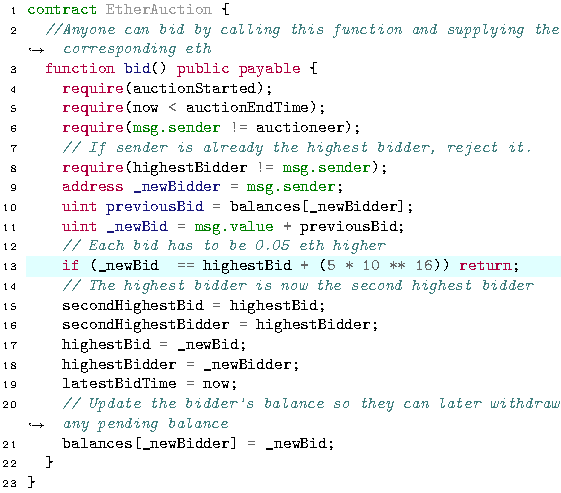
\includegraphics[width=\columnwidth]{Figures/Chapter2/EtherAuction.pdf}
	\caption{The EtherAuction Solidity source code.}\label{fig:etherauction}
\end{figure}


\cref{table:voting} shows the result of property checking for the selected five voting smart
contracts, each of which is for five voters and two proposals. The first column shows the names of
contracts. The last column, $t_{model}$, shows the model extraction time (in seconds). The middle
two large columns show the average property checking time (in seconds) for the three properties:
truthfulness (T), collusion-freeness (C) and efficiency (E). We have two settings for the valuation
component in our mechanism model. One is ranging over real numbers $\mathbb{R}$, while the other is
ranging over $\{0, 1\}$. The reason of having two settings is that no contract was found fair
regarding any property, as shows in the second large column of \cref{table:voting}, because
the diverse $\mathbb{R}$ valuation of proposals brings the incentive for voters to lie and to
conspire with others. In the $\{0, 1\}$ valuation setting, as shows in third large column of
\cref{table:voting}, all the five contracts are truthful, collusion-free, and efficient. This is
because, if a voter lies, he/she gets at most zero worth utility, and thus has no incentive to lie.
Based on \cref{table:voting}, we can observe that fairness property may depend on the configuration
of mechanism models. Different configurations may have different results on fairness property
checking.

The checking time for the optimality property is not listed in \cref{table:voting} because
smart contracts for voting do not have the component of transfer functions in our mechanism model
so that optimality cannot be defined (c.f. \cref{subsec:FairnessProperty}). In addition, none of
the predefined invariants are valid to prove that the five selected voting contracts are fair. We
need to construct other valid invariants manually, which is one of our future works.

%For 2 voter collusion, because 2 voters account for less than half of the voters and are not responsible for the final result, voter cannot be incentivized to collude with another one without any utility increase. Since voter votes his preferred proposal, the most preferred proposal would be the winning proposal in the end, making the voting efficient.


%Regarding the execution time for model extraction and property checking, we can observe that model extraction is the bottleneck of our framework, and property checking is efficient (less than one second for each case). All the results will be available on the website: \url{https://sites.google.com/view/fse2020-faircon}.

%\liu{Since there's a lack of ground truth, we manually investigate our cases and the results.
%Each counterexample, for unfair case, has been examined and successfully replayed.
%The proofs, including the invariants used, has also been checked carefully and confirmed.}
\begin{tcolorbox}[size=title, opacityfill=0.1]
	\textbf{Answer to RQ1}:
	Since there is a lack of ground truth, we manually investigated the cases and the results of \faircon
	were confirmed.
	%We conclude that \faircon is accurate.
\end{tcolorbox}

%\begin{tcolorbox}[size=title, opacityfill=0.1]
%  \textbf{Answer for Q1}: Out of 12 auction contracts, we found 8 contracts are not fair for all four fairness properties and 3 contracts are proved for their fairness properties and 1 contract had not been proved because of invariant missing.
%  We manually inspected generated counterexamples to verify these unfair cases. By using allocation
%  invariant and price invariant, we carefully produced and manually verified the proof for fairness
%  property for those fair cases.
%  For 5 voting contracts, they are unfair when the valuation of voter to proposal is in real domain and behave fair for three fairness properties when the valuation is 0 or 1.
%\end{tcolorbox}



\begin{figure}[t]
	\centering
	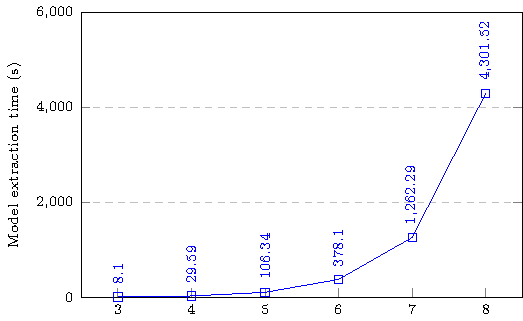
\includegraphics[width=.95\columnwidth]{Figures/Chapter2/modeling-figure0.pdf}
	\caption{Model extraction time with increasing number of bidders.}\label{fig:model-time}
\end{figure}

\begin{figure}[t]
	\centering
	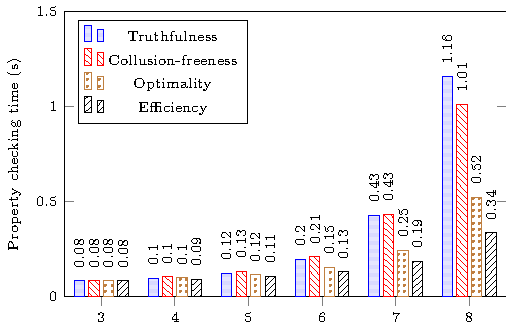
\includegraphics[width=.95\columnwidth]{Figures/Chapter2/checking-figure0.pdf}
	\caption{Property checking time with increasing number of bidders.}\label{fig:check-time}
\end{figure}

\paragraph{Results for RQ2}
The time costs studied in RQ2 can be divided into two parts: model extraction and property
checking.
Overall, the model extraction takes much longer time and the property checking is efficient
(taking less than one second for each case), as shown in \cref{table:auction,table:voting}.

To explore the efficiency of \faircon further, we selected the \texttt{CryptoRomeAuction} contract to
make performance experiments on \faircon.
\Cref{fig:model-time,fig:check-time} show the execution time for mechanism model extraction and
fairness property checking when the number of bidders increases, respectively.
In \cref{fig:model-time}, the x-axis shows the number of bidders, while the y-axis shows the
mechanism model extraction time in seconds. We can observe that model extraction time is nearly
exponential to the number of bidders involved, which is reasonable because every participant is
independent.
When the number of bidders is under six, the model extraction time is less than 10 minutes, which
is tolerable. Once the number of bidders goes beyond six, the time increases exponentially.

\Cref{fig:check-time} shows the property checking time, where the x-axis indicates the number of
bidders, and the y-axis indicates the property checking time in seconds. We can observe the same
trend as that in \cref{fig:model-time}, i.e., the execution time is exponential to the number
of bidders involved. However, property checking is much faster than model extraction since model
extraction requires symbolic execution, which is heavy in computation. Mostly the checking time is
less than one second. We can also observe that the checking time for truthfulness or
collusion-freeness is at least doubled than that for optimality and efficiency. This is because
truthfulness and collusion-freeness properties need to consider the strategy as well as the outcome
spaces, while optimality and efficiency properties only have to consider the outcome space.

%When the number of bidders increases, the time slightly goes up. Looking at the checking time for different fairness properties, taking truthfulness and optimality as an example, we observe there is no significant difference in the checking time between of truthfulness and of optimality when the number of bidders is below 6. However, the time used for checking truthfulness is nearly twice the time used for checking optimality in 7-bidders auction or 8-bidders auction. As mentioned in Sect. ~\ref{section:experiment-setup}, checking optimality actually compares the outcome of current mechanism model with the outcome of a virtual mechanism model, but checking truthfulness needs to compare the outcome of the current mechanism model and its mirror model. The current mechanism model is ideally truthful and the mirror is untruthful one. So the complexity of SMT formula for checking truthfulness is larger than that for checking optimality, thus causing the time use difference.

%In summary, \faircon performs pretty fast in the phase of fairness property checking and if we want to verify the smart contract having more than 6 participants, invariant should be in use as a more effective measure.

%\liu{The time costs studied in Q2 can be divided into two parts: model construction (Fig.8) and
%property checking (Fig.9).
%%Indeed, the model extraction time increases exponentially, and the property checking time does increase with the growing number of bidders, but is generally fast (around one second).%The experimental goal is not to run \faircon on a large number ($k$) of participants, which is theoretically
%%unbounded. \faircon can usually find counterexample(s) even with small $k$ (e.g.,
%%3 or 5),
%%if the contract is indeed unfair ($k$=3 in Table:2 and $k$=5 in Table:3).
%%Otherwise, \faircon
%%uses invariants observed during the $k$ runs to try to prove the fairness property holds for an
%%arbitrary $k$.
%}

Running \faircon on a large number (i.e., $k$, which is theoretically unbounded) of players is
impractical for symbolic execution.
The results indicate that \faircon can finds counterexample(s) with small $k$ (e.g., three to five),
if the contract is indeed unfair (e.g., $k=3$ in \cref{table:auction} and $k=5$ in
\cref{table:voting}).
Otherwise, as shown in~\Cref{table:proof}, \faircon could use invariants observed during the small $k$
runs in an attempt to prove that the fairness property holds for arbitrary values of $k$.
%\yi{Although model extraction time increases exponentially with more players, we do not intend to
%run \faircon on a large number ($k$) of players, which is theoretically unbounded.
%Our experience is that \faircon often finds counterexample(s) with small $k$ (e.g., 3 to 5), if the
%contract is indeed unfair (e.g., $k=3$ in \cref{table:auction} and $k=5$ in \cref{table:proof}).
%Otherwise, \faircon uses invariants observed during the $k$ runs to try to prove the fairness property
%holds for an arbitrary $k$.}

\begin{tcolorbox}[size=title, opacityfill=0.1] \textbf{Answer to RQ2}:
	Although model extraction is the bottleneck of \faircon, it is a one-time task and need not be
	performed for a large $k$.
	\faircon is efficient for fairness property checking.
\end{tcolorbox}

%\begin{tcolorbox}[size=title, opacityfill=0.1] \textbf{Answer for Q2}: Difference lies in the
%efficiency of mechanism model construction and the efficiency of fairness property checking.
%Increasing the number of participants, due to exponentially increasing complexity of mechanism
%model, the time used for mechanism model construction goes up nearly exponentially. However,
%fairness property checking runs very quickly and the time used is usually below one second.
%\end{tcolorbox}

\paragraph{Results for RQ3}
%\yi{This needs to be rewritten.}
%<<<<<<< HEAD
%\liu{Based on our review of the subject contracts, we have summarized some common unfair patterns
%as below.
%We hope the common patterns could raise developers' awareness of fairness issues while developing
%smart contracts.
%We also hope that fairness checking will be included as a part of the common-practice validation process to improve users' confidence towards such applications.
%For example, EtherAuction (as shows in \cref{fig:etherauction}) was reported as a
%scam,\footnote{\url{https://hackernoon.com/take-your-chances-at-the-ether-auction-game-30f9df1ec80b}}
%where bidders compete for 1 Ether by gradually increasing their bids.
%Our results confirmed its unfairness: although truthfulness/collusion-freeness holds for bounded k, optimality and efficiency are violated.
%Therefore, the real-world fairness risk is not far and could be mitigated by alerting developers or
%users through some high level summarization of common unfair patterns.
%=======
%We would like to study the common patterns of unfair contracts to raise the awareness of fairness
%issues in smart contract development.
Fairness issues in smart contracts are real.
For example, \texttt{EtherAuction} (as shows in \cref{fig:etherauction}) was reported as a
scam,\footnote{\url{https://hackernoon.com/take-your-chances-at-the-ether-auction-game-30f9df1ec80b}}
where bidders compete for one Ether by gradually increasing their bids.
Our results confirmed its unfairness: although truthfulness and collusion-freeness holds for a
bounded $k$, optimality and efficiency are violated.
Based on our review of the subject contracts, we summarize some patterns below.
%>>>>>>> save fixes
%Based on our review of the subject contracts, we have summarized some common reasons causing
%fairness violations.
%which may help
%the participants of smart contract quickly know whether the contract is unfair. The patterns are
%following.

\begin{enumerate}[leftmargin=*]
	\item Contracts implementing the first price auction and their variants do not satisfy the
	truthfulness property.
	For example, the aforementioned \texttt{BetterAuction} is implementing a typical open first
	price auction, where the top bidder has the incentive to lower his/her bid price but still
	remain the winner.
	\item Contracts implementing the first price auction and variants do not prevent against
	collusion.
	For example, \texttt{BetterAuction} does not satisfy the collusion-freeness property, since two
	bidders have the chance to lower the clear price and to be the winner, increasing their
	group utility.
	\item Contracts implementing the second price auction and their variants do not satisfy the
	optimality property.
	For example, \texttt{Deed} is one of the contracts implementing the second price auction.
	Since the clear price is the second highest bid, the contract may not be optimal with a potential
	decrease in total revenue.
	\item Contracts implementing the first price auction and their variants are not efficient.
	This is because first price auctions are untruthful, and the winner may not be the one who has
	the highest valuation of the item.
	%\texttt{BetterAuction} is unfair for efficiency property as well.
\end{enumerate}

We envision that fairness checking be included as a part of the common-practice validation process
to improve users' confidence towards DApps powered by smart contracts.
We hope the fairness issues in smart contracts can be mitigated by alerting developers and users
these common patterns.

\subsection{Threats to Validity}

Our evaluation results are subject to common threats to validity.
\paragraph{Lack of ground truth}
%  Smart contract is an emerging technology in recent years. However, there are no
%labeled smart contracts suitable for our
%  fairness analysis.
It lacks ground truth for the contracts and properties we studied.
Two of the authors manually inspected the subjects and our results independently, which
took around half an hour for each contract.
We confirmed that the counterexamples provided by our tool are valid.

\paragraph{External validity}
The types of contracts and properties considered in this work are limited.
Our findings may not be generalized to other cases.
The DApps implemented with smart contracts usually follow typical patterns, mainly due
to the limitations on language syntax and considerations on gas consumption.
We believe that other types of game-like contracts would behave similarly.
%  We have limited configurations in our experiments and this would prevent us from
%  having more sights of fairness property of smart contract.
%  Although we do not consider the cases where the bid distribution of bidder is
%  nonrandom, we conduct our experiments with different number of bidders (3 to 8) and
%  for voting we have 5 voter and 2 proposals.
%  We also consider two possible scenario where the voter's valuation of proposal is
%  customized differently. In this way, we could relieve the configuration bias to some
%  extent.
%  Actually, as part of the solution, user should offer their customized configuration
%for
%  fine-grain mechanism analysis.
\section{Related Work}\label{Sec_RelatedWorks}
%In this section, we briefly summarize research works related to smart contract analysis and
%verification in \cref{subsec:AnalysisVerification}.
%Research works on applying mechanism design or game theory on smart contracts are summarized in
%\cref{subsec:MechanismDesign}.

Our work is closely related to the following research areas:
(1) the functional correctness and security analysis of smart contracts,
(2) the verification of fairness properties in traditional software systems,
(3) and mechanism design as well as game theory.


\subsection{Smart Contract Analysis and Verification}\label{subsec:AnalysisVerification}

Since smart contract applications are often used to manage a large sum of funds, detection of
security flaws in smart contracts received a lot of attention.
%Important security properties studied by the research community include \emph{liquidity} (``a
%non-zero contract balance is always eventually transferred to some
%participants~\cite{Nikolic2018,Bartoletti2019}''),
%\emph{atomicity} (``if one part of the transaction fails, then the entire transaction fails and the
%state is left unchanged''~\cite{Luu2016}), \emph{single-entrancy} (``the contract cannot perform
%any more calls once it has been reentered''~\cite{Schneidewind2020}), \emph{independence of the
%  mutable state and miner-controlled parameters}~\cite{Grishchenko2018,Wang2019payment}.
%Security guarantees of a smart contract also include proper \emph{access
%  control}~\cite{Tsankov2018,Nikolic2018} for safety-critical operations,
%% such as cryptocurrency transfers
%\emph{arithmetic correctness}~\cite{So2019,Feng2019a,Kalra2018}, and
%\emph{reasonable resource consumption}~\cite{Bhargavan2016,Chen2017,Grech2018}.
%The similarity of a smart contract to a concurrent object~\cite{Sergey2017} suggests that some
%security guarantees can be derived from checking for \emph{linearizability}~\cite{Kolluri2019} and
%\emph{serializability}\cite{Grossman2017} of its executions.
The violation of important security properties leads to many well-known smart contract
vulnerabilities~\cite{tolmach2020survey}.
For example, a smart contract which fails to check the return value of a (possibly failed) external
call operation, has the \emph{unchecked call}
vulnerability~\cite{grishchenko2018semantic,Perez2019}.
The execution logic of a smart contract that is not independent of environmental variables,
e.g., the block timestamp, is prone to \emph{dependence manipulation}~\cite{Wang2019payment},
including the \emph{timestamp dependency} vulnerability~\cite{luu2016making}.
If the business logic of a smart contract depends on its mutable state parameters, such as balance
and storage, then it has the \emph{transaction-ordering dependence} problem.
A smart contract is \emph{reentrant}, if provided with enough gas, an external callee can
repeatedly call back into it within a single transaction.
Missing permission checks for the execution of a \texttt{transfer} or a \texttt{selfdestruct}
operation make a smart contract \emph{prodigal} and \emph{suicidal},
respectively~\cite{nikolic2018finding}.
Absence of proper checks for arithmetic correctness make Ethereum contracts prone to
\emph{integer and batch overflow/underflow}~\cite{So2019,feng2019precise}.
Furthermore, the progress of a smart contract can be compromised by gas-exhaustive code
patterns~\cite{Chen2017,grech2018madmax}.

%\subsubsection{ Vulnerable Smart Contract }
%
%Smart contract development is very different from traditional programming such that developers tend
%to write vulnerable smart
%contracts.
%Delmolino et al.~\cite{delmolino2016step} first exhibited that a tiny smart contract can still
%contain a lot of logical problems such as contract never refunding to its sender and privacy
%leakage.
%Atzei et al.~\cite{atzei2016survey} surveyed and analyzed large amounts of existing attack reports,
%and then offered relatively comprehensive taxonomy of smart contract vulnerabilities based on
%different occurring contexts and characteristics.
%To reduce the security risk of smart contracts, Wohrer et al.~\cite{wohrer2018smart} claimed some
%practical programming-centered security patterns to prevent smart contracts from attacks.
To address these security issues, Ellul et al. developed a runtime verification technique,
ContractLarva~\cite{ellul2018runtime}, to rule out certain unsafe behaviors during the execution of
smart contracts.
%Since vulnerable smart contracts lead to huge financial losses,
%security tools were booming to enhance security or detect vulnerabilities of smart contracts.
Oyente~\cite{oyente,luu2016making} is one of the first to detect smart contract vulnerabilities
using symbolic execution.
ContractFuzzer~\cite{jiang2018contractfuzzer} is among the early fuzz testing tools and
Mythril~\cite{mythril} is a well-known security analysis tool which combines symbolic execution and
taint analysis to detect nearly 30 classes of vulnerabilities.
There are many other
tools~\cite{kalra2018zeus,SmartCheck,securify,tsankov2018securify,chang2018scompile,wang2019vultron,Wang2019b}
designed for the similar purpose.
%and empirical analysis~\cite{parizi2018empirical} to the tools mentioned above.
%\liu{However, most of the smart contract analysis focuses on finding bugs or security
%vulnerabilities, which	highlight mismatches between developers' expectations and how the contract
%code actually	works; whereas the fairness issues considered in our paper highlight mismatches
%between the	participants' expectations and the actual implementation of the game rules}

%	most of the studied vulnerabilities are related to the security or correctness aspects of smart contract. In this paper, we focus on smart contract fairness properties.

%Different from existing these works, our work is the further analysis established on the basis of these researches. The smart contracts we analyze are not vulnerable using these method, but they have some unfairness properties for the user, which can be utilized by the malicious user to get revenue. And to our knowledge there is no related work involved.

Another popular direction is using formal techniques to ensure the functional correctness of smart
contracts.
Bhargavan et al. devised a functional programming language, named $F^*$~\cite{bhargavan2016formal},
to facilitate the formal verification of Ethereum smart contracts.
%The verification is done by translating source code and bytecode to $F^*$ programs, respectively,
%and checking their consistency.
Based on $F^*$, Grishchenko et al. presented the first complete small-step semantics of EVM
bytecode~\cite{grishchenko2018semantic}.
%They applied their semantics to verify smart contract against some security properties such as
%call integrity, atomicity, and independence from miner controlled parameters.
%Hirai~\cite{hirai2016formal} provides a formal proof case study for the smart contract.
%This work exploited Isabelle/HOL proof tool to verify a smart contract named \texttt{Deed}, and the
%result implied a malicious problem that only the owner of \texttt{Deed} can decrease the balance.
Hildenbrandt et al. presented an executable formal semantics for the Ethereum platform, named
KEVM~\cite{hildenbrandt2017kevm}, based on which, Park et al.~\cite{park2018formal} presented a
deductive verification tool, capable of verifying various high-profile and safety-critical
contracts.
Jiao et al. developed the operational formal semantics for the Solidity programming language, named K-Solidity~\cite{JKL20, JLS20}. Abdellatif et al.~\cite{abdellatif2018formal} formalized blockchain and users' behaviors to verify
properties about their interactions using statistical model checking.
Nehai et al.~\cite{nehai2018model} applied model checking to verify smart contracts from the energy market field.
%\liu{However, most of the studies apply traditional formal verification methods to smart contract,
%which are incompetent to deal with the fairness properties in our paper.}
%\yi{Try not to start with ``However'', at least for some of them.}

Most of the smart contract analyses mentioned above focus on finding bugs or security
vulnerabilities, which highlight mismatches between contract developers' expectations and how the
contract code work; whereas the fairness issues considered in our paper highlight mismatches
between the contract users' expectations and the actual implementation of the game rules.

%Our work also can be regard as checking the malicious smart contracts, but different  from these works, we mainly focus on the mechanism design problems which are fairness properties rather than the safety properties, where these fairness properties can cause implicitly detrimental for the users.


%\liu{Fairness plays a key role in smart contract design.}
%There are some researches on the smart contract design problem.
%Nikoli{\'c} et al.~\cite{nikolic2018finding} identified and analyzed three vulnerabilities of smart
%contracts: prodigal, greedy and suicidal.
%They proposed a tool, called \textit{MAIAN}, for symbolic analysis of smart contract bytecode and
%test (close to) one million contracts.
%The result showed that there is a wide distribution of thousands unreliable contracts.
%\liu{However, \textit{MAIAN} can only help with very simple function correctness problems;
%whereas in our paper, we cope with contract-level fairness design problem.}
%Our work also focus on the smart contract design problem, but different from these
%works, we mainly focus on the mechanism design problem behind the smart contract rather
%than the coding design problem. Therefore, the unfairness smart contracts we detected
%are safety using these works to check.

\subsection{Fairness Checking in Software Systems}

We believe that fairness should be considered a software quality attribute---among functional
correctness, security, privacy, etc.---one needs to consider throughout the software development
process.
Smart contract is an emerging type of software application with often multiple interacting
participants, where fairness becomes a lot more relevant.

The problem of \emph{algorithmic fairness} is considered in many modern decision-making
programs~\cite{zemel2013learning,datta2016algorithmic,Albarghouthi2017FairSquarePV}, either learned
from data or created by experts.
The term ``fairness'' can be subjective depending on the actual contexts.
Verma and Rubin~\cite{VR18} collected definitions of fairness from different software domains and
explained the rationales behind these definitions.
From the software specification and verification perspective, Albarghouthi et
al.~\cite{Albarghouthi2017FairSquarePV} treated decision-making algorithms as probabilistic programs
and proposed to verify formally defined fairness properties on a wide class of programs.
D'Antoni et al.~\cite{Albarghouthi2019FairnessAwareP} introduced the concept of
\emph{fairness-aware programming} and presented a specification language and runtime monitoring
technique which allow programmers to specify fairness properties in their code and enforce the
properties during executions.
In general, the fairness definition in such decision-making programs is that the program shows no
bias towards certain groups of users.
There is little consideration in terms of the interactions, interests, and conflicts between
users and programs, or between users and users.

With regard to smart contracts, Bartoletti et al.~\cite{bartoletti2019dissecting} found through a
survey that nearly $0.05\%$ of the transactions on Ethereum could be owing to Ponzi schemes.
Chen et al.~\cite{chen2018detecting} identified patterns in contract applications implementing
Ponzi schemes, and built a classifier to detect suspicious schemes using data mining and machine
learning.
%Kalra et al.~\cite{kalra2018zeus} presented the most relevant work of ours.
%They integrated abstraction interpretation with symbolic model checking to attain the execution
%semantics of smart contracts, and then presented a symbolic model checking framework, named
%\textit{ZEUS}, for verification of correctness and fairness policies.
%They evaluated over $22.4$K Solidity smart contracts and found that about $94.6\%$ of them are
%vulnerable.
%However, the fairness they considered is only for the coding logic correctness, instead of the
%whole mechanism design fairness properties discussed in our paper.
Such contracts can be considered violating fairness properties, in the sense that not all
participants have the same chance of gaining profits.
In this work, we expand the notion of fairness in smart contracts to include any properties
expressible in mechanism models.

\subsection{Mechanism Design and Game Theory}\label{subsec:MechanismDesign}
%\subsubsection{Mechanism Design Problem}

Mechanism design has been well studied in the economic
domain~\cite{maskin2008mechanism,jackson2014mechanism,klemperer1999auction,lehmann2002truth}.
These works offer the theoretical foundation for our model extraction and fairness verification.
Many fairness properties we used in this paper are also inspired by them.
Maskin~\cite{maskin2008mechanism} articulated some important concepts, such as \textit{outcomes}
and \textit{social goals}, in implementation theory, which is a part of mechanism design.
He offered a well-defined example to show how to achieve social goals.
Jackson~\cite{jackson2014mechanism} presented mechanism theory in a full view and provided formal
definitions to many concepts belonging to this domain, while Klemperer~\cite{klemperer1999auction}
introduced the most fundamental concepts for auction and carried out a thorough analysis of optimal
auctions, the equivalence theorem, and marginal revenues.
Lehmann~\cite{lehmann2002truth} revealed how to exploit truth revelation in realizing approximately
efficient combination auction which emphasized the co-exist problem of \textit{optimal} auction and
\textit{efficient} auction.

%Nisan et al.~\cite{nisan2001algorithmic} might be the most famous to draw mechanism design to
%algorithmic problems analysis, which greatly bridged the solution between mechanism design and
%algorithmic design such as task scheduling problems.

%In this paper, based on these previous work, we devise the mechanism model to adapt the analysis of smart contract, so that we can check some fairness properties we proposed which are critical for the smart contract users.

%\subsubsection{Mechanism and Game Theory in Smart Contract}

%As for the smart contract, previous works mainly focus on using the mechanism and game
%theory to design an application on the smart contract.

Mechanism design and game theory were also applied on the smart contract design.
Hahn et al.~\cite{hahn2017smart} implemented a Vickrey second price auction on a smart contract to
setup and operate a market of energy exchanges.
Similarly, Chen et al.~\cite{chen2018blockchain} provided an e-auction mechanism based on
blockchain to ensure confidentiality, non-repudiation, and unchangeability of the electronic sealed
bid.
CReams~\cite{wu2018cream} implemented a collusion-resistant $k$-Vickery auction.
Galal and Youssef~\cite{galal2018succinctly} presented a smart contract protocol for a succinctly
verifiable sealed-bid auction on the Ethereum blockchain to protect bidders' privacy.
Mccorry et al.~\cite{mccorry2017smart} proposed the first implementation of a decentralized and
self-tallying internet voting protocol using smart contract to guarantee secure e-voting.
Bigi et al.~\cite{bigi2015validation} combined game theory and formal models to analyze and
validate a decentralized smart contract protocol, named \textit{DSCP}, and used game theory to
analyze users' behavior.
Chatterjee et al.~\cite{chatterjee2018quantitative} studied two-player zero-sums games and
performed a quantitative analysis of players' worst case utilities.
These works employ certain levels of fairness analyses, mostly manual, on some one-off applications.
In contrast, we provide a more general framework with maximal automation support.



%\liu{However,} the type of analysis they do only works for the two-player case.
%\liu{And both the studies fail to formally present mechanism fairness properties concerning smart
%contract, which make it a little hard to apply in general scenarios.}
%In contrast, we use a general mechanism model to check fairness properties for many kinds of Ethereum smart contracts.

%However, different from these works focus on the application, our work focuses on using mechanism models to detect the fairness of smart contracts.

\section{Conclusion and Future Work}\label{Sec_Conclusion}
In this paper, we proposed an approach to analyze fairness properties of smart
contracts.
We implemented \faircon to automatically extract mechanism models from smart contracts with
user-provided annotations, and experimentally evaluated it on 17 real-world auction and
voting contracts.
The experiment results indicate that \faircon is effective in detecting property violations
and able to prove fairness for common types of contracts.
%Therefore, with the assistance of \faircon, it will not be difficult for participants to
%understand
%the underlying fairness issue of the smart contract, which the participants will play a
%role in.
%And \faircon will help smart contract creators identify potential risks when setting up
%smart contract applications such as auction or voting.

In the future, we would like to apply \faircon to other types of smart contracts beyond
auction and voting.
It can also be extended to check for other types of fairness properties that are critical
in maintaining the integrity of blockchain applications.


%!TEX root=../mythesis.tex
% Chapter Template

\chapter{Model-Based Testing Platform for Smart Contract} % Main chapter title
\chaptermark{ModCon: Model-Based Test Platform for Smart Contract}  % replace the chapter name with its abbreviated form
\label{ch:modcon} % Change X to a consecutive number; for referencing this chapter elsewhere, use \ref{ChapterX}



%-----------------------------------
% SECTION 1
%-----------------------------------
\section{Introduction}
\label{sec:intro}

Smart contracts are computer programs that execute on top of blockchains (e.g.,
Ethereum~\cite{Ethereum}) to manage large sums of money, carry out transactions of assets, and
govern the transfer of digital rights between different parties.
Transactions conducted through smart contracts are recorded on blockchains, thus decentralized and
immutable, without requiring validation from a central authority.
Due to these unique advantages, smart contracts have gained much popularity in recent years.
Many believe that this technology has the potential to reshape a number of industries,
e.g., banking, insurance, supply chains, and financial services~\cite{iansiti2017truth}.

The existing blockchain networks can be broadly categorized into the permissionless and
permissioned blockchains, where the former is open to the public (e.g.,
Bitcoin~\cite{nakamoto2008bitcoin} and Ethereum~\cite{Ethereum}) and the latter is only accessible
to trusted private groups or individuals (e.g., Hyperledger Fabric~\cite{hyperledger-fabric}).
The consortium/federated blockchains (e.g., FISCO BCOS~\cite{fisco} and Azure Blockchain
Workbench~\cite{azure-workbench}) sit somewhere in the middle: they are suitable for use between
multiple businesses or organizations for performing  transactions and exchanging information.
One major difference between smart contracts on the permissioned and permissionless blockchains is that the
contract execution on permissionless chains is bounded by resource constraints.
For example, on Ethereum, one has to pay miners a certain amount of ``gas'' (cryptocurrency on Ethereum) as the transaction fee to deploy or call contract, which is largely decided by the complexity of the contract (e.g., up to \$15 in fees~\cite{gas-fee}).
%relative to the complexity of the contract, in order to have the execution results confirmed and accepted by the blockchain.
Therefore, to reduce the gas consumption, smart contracts on permissionless chains are often kept simple, making it
unsuitable for implementing enterprise applications with complex business logic.

At the same time, smart contracts have been used to implement many industrial applications of high
complexity and production quality on permissioned and consortium blockchains.
Unlike the permissionless blockchains, such as Bitcoin and Ethereum mainly used for cryptocurrency
exchange (e.g., ERC Token and DeFi applications), the permissioned blockchains aim to create real
value.
For instance, FISCO BCOS has been successfully adopted in areas such as government and judicial services, supply chain, finance, health care, copyright management, education, transportation, and
agriculture~\cite{fisco}.
The smart contracts powering these applications are more sophisticated and often demonstrate strong
stateful behaviors.

\paragraph{Example}
\Cref{fig:scenario} illustrates some usage scenarios of a Credit Management Application (\wecredit)
at \company~\cite{webank}, implemented using smart contracts, running on FISCO BCOS consortium
blockchain.
%We hereafter refer to it as \wecredit.
\wecredit is used to handle inventory and asset management in supply chain through a blockchain-based credit system,
which can facilitate credit transfer among different business owners and help small
businesses receive instant financial support securely.

\begin{figure}[t]
	\centering
	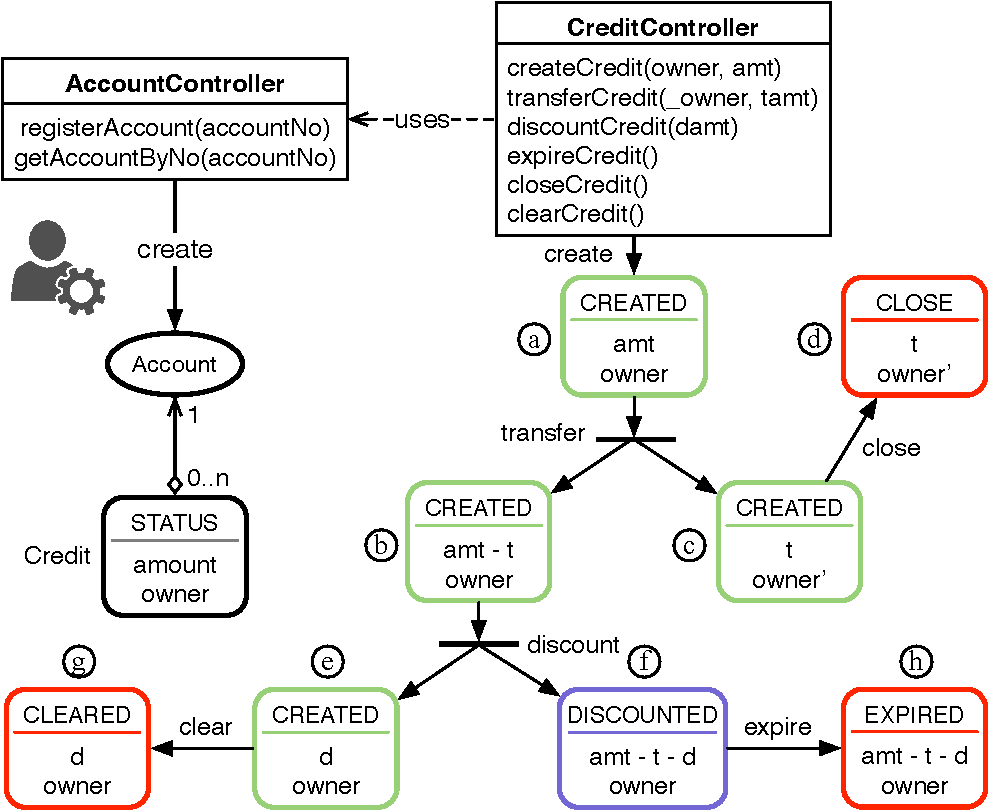
\includegraphics[width=.80\columnwidth]{Figures/Chapter3/modcon.pdf}
	\caption{Illustration of a \wecredit smart contract at \company.}
	\label{fig:scenario}
\end{figure}

The user first deploys an \code{AccountController} contract, whose address is then used to
instantiate the \code{CreditController} contract.
\code{AccountController} is in charge of the account creation and management.
An account may own \code{Credit}(s), which are transferable and divisible tokens with stipulated values.
The state of a \code{Credit} is captured by the tuple, $(\mathit{STATUS},amount,owner)$, whose
fields represent the status, value captured, and its ownership, respectively.
A \code{Credit} instance supports credit operations including creation, transfer, discount, expiration, clearance, and closure.
Through \code{CreditController}, one can first create a credit, namely, \textcircled{a},
under the specified \code{Account}.
In this case, a \code{transfer} operation is executed on \textcircled{a}, thus dividing
\textcircled{a} into two new credits, namely, \textcircled{\raisebox{-.9pt}{b}} and \textcircled{c}.
By design, the total value of \textcircled{\raisebox{-.9pt}{b}} and \textcircled{c} equals to that
of \textcircled{a}.
Then a \code{discount} operation is applied on \textcircled{\raisebox{-.9pt}{b}}, resulting in
a newly created credit \textcircled{e} and a discounted credit \textcircled{\raisebox{-.9pt}{f}}.
By design, the total value of \textcircled{e} and \textcircled{\raisebox{-.9pt}{f}} equals to that
of \textcircled{\raisebox{-.9pt}{b}}, but the status of \textcircled{\raisebox{-.9pt}{f}} becomes
``DISCOUNTED''. %which is different from \textcircled{\raisebox{-.9pt}{e}} marked as ``CREATED''.
To complete the life cycle of a credit, one may apply either the \code{close}, \code{clear}, or
\code{expire} operation, bringing the credit into the ``CLOSED'' (e.g.,
\textcircled{\raisebox{-.9pt}{d}}), ``CLEARED'' (e.g., \textcircled{\raisebox{.9pt}{g}}), or
``EXPIRED'' (e.g., \textcircled{\raisebox{-.9pt}{h}}) state, respectively.
Once a credit is in ``CLOSED\allowbreak{}/CLEARED\allowbreak{}/EXPIRED'', it should no longer
accept further operation.

%\yi{Let's not focus on FISCO BCOS so much. In principle, the modcon also work on Ethereum. We just
%use FISCO as an industrial case study.}
%FISCO BCOS~\cite{fisco} is a secure and reliable financial-grade open-source blockchain platform
%led by Chinese enterprises.
%Its performance, usability, and security have been testified by many institutional users and
%successful business applications in a live production environment.
%FISCO BCOS has been adopted in over 10 applications in areas like government affairs, finances,
%charity, health care, education, transport, copyright, product tracing, supply chain, recruitment,
%agriculture, social communication, and entertainment.
%\par

%Smart contracts are at the core of these applications on FISCO BCOS blockchain.
%Similar to Ethereum, FISCO BCOS supports writing smart contract using Solidity programming
%language.
%Since writing secure smart contract is non-trivial, which requires programmers have a comprehensive
%understanding of smart contract language and blockchain platform principles, etc,
%there are considerable number of smart contract attacks~\textcolor{red}{XXX atacks} in recent
%years.
%Testing or verifying smart contracts appeals greatly to the research
%community~\textcolor{red}{Testing or verifying researches}.

Existing testing and analysis tools target Ethereum smart contracts and mainly focus on their
security issues.
Such tools do not work well on this example for the following reasons.
\textbf{(1) Lack understanding of system behaviors}.
The different states of a credit instance is implemented with special encoding.
For example, the $\mathit{STATUS}$ field is encoded as bit-vectors for performance considerations.
It is unclear how to interpret system states and behaviors at these states without this knowledge.
\textbf{(2) Absence of oracle}.
Existing tools may rely on implicit security properties (e.g., underflow/overflow and exceptions)
as oracle, which is absent when the functional correctness is concerned.
The expected system behavior (e.g., ``EXPIRED'' is terminal) is not known prior and should be
provided by the contract designer.
\textbf{(3) Missing measurement of test adequacy}.
The traditional coverage criteria used by existing tools, such as branch and path coverage, are not
good measurement of test adequacy for this example.
Covering every single path of the contract program does not equal exercising all system states and
state transitions.
It is challenging to navigate through all system behaviors without proper adequacy measurements.

%\yi{Let's not sell FISCO BCOS, which is not so well-known. The selling point should be model-based
%testing.}
%However, most existing research tools support only testing smart contract on Ethereum.
%Smart contracts on FISCO BCOS are industrial applications of high complexity and high value beyond
%those on Ethereum.
%Generating smart contracts automatically could ensure the security of smart contracts to some
%extent by well-defined formal models such as state machine model \textcolor{red}{ref}.
%However, most available smart contracts are usually not generated full-automatically by model
%specification.
%Testing remains an effective measure to verify whether there is any violation against model
%specification of smart contract.
%\par

\paragraph{\modcon}
To address these challenges, we propose \modcon, a model-based testing platform for smart contracts.
\modcon targets enterprise smart contract applications written in Solidity~\cite{solidity} from permissioned/consortium blockchains such as FISCO BCOS, but is also compatible with Ethereum.

\modcon allows users to specify system models and define test oracles, which are then used to guide
the test generation and execution.
%which firstly supports FISCO BCOS (\textcolor{red}{not sure as well as Ethereum}).
%\modcon is a Web-based testing framework, which provides basic workflow( Uploading, Compiling,
%Deployment, Query/Transaction ) to interact with smart contracts on FISCO BCOS.
%\modcon enables smart contract testing once user provides the model specification of smart contract
%while \modcon allows for testing strategy or test case priority specified by user.
The key features of \modcon include the following.
\begin{itemize}[leftmargin=*,topsep=2pt]
	\item \textbf{Test-Model Specification}.
	\modcon allows users to provide a test model for the target smart contract.
	The model is used to specify the state definitions, expected transition relations,
	pre/post conditions to be satisfied for each transition, invariants, and the mapping from the
	model to the contract code.
	\item \textbf{Customized Test Generation}.
	With the test model given, users can further customize the testing process by choosing from
	different coverage strategies and test prioritization options.
	\modcon then generates tests with the goal of exercising as many system behaviors as possible while
	prioritizing on cases of particular interests.
	Any violation of the specified oracle is recorded and reported to users.
	\item \textbf{Web-Based Interface}.
	\modcon has a Web-based interface, providing easy access to all the testing capabilities and
	customization options.
	Source code and a video demonstrating the usage of \modcon are available at \modconurl.
	%  \modcon is data driven which could make the testing process to be perceived easily.
\end{itemize}
%\par


\section{\modcon Overview}
\label{sec:Overview}

\begin{figure}[t]
	\centering
	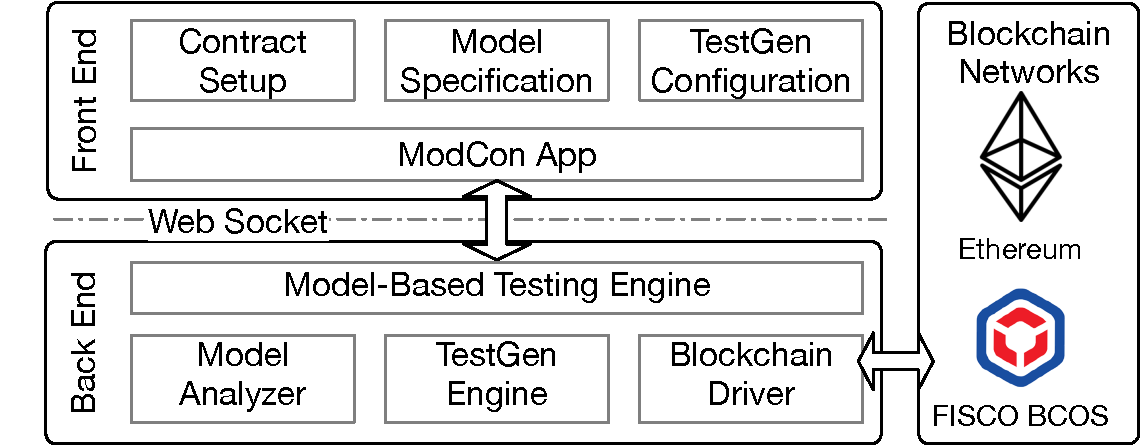
\includegraphics[width=.9\columnwidth]{Figures/Chapter3/modcon-arch.pdf}
	\caption{Architecture of \modcon.}
	\label{fig:architecture}
\end{figure}

In this section, we describe the architecture of \modcon and demonstrate its user interface.
As shown in \cref{fig:architecture}, \modcon consists of a web-based front end (implemented as a
Vue.js~\cite{vuejs} application) and a server-side back end (implemented on top of the Node.js
JavaScript runtime~\cite{nodejs}).
The front-end accepts two inputs from users: the target smart contracts
%which will then be compiled by \modcon and deployed to blockchain platforms.
and the test-model specifications to drive the model-based testing process.
The front-end allows users to specify coverage strategies and configure test generation priority,
and the test execution progress can be monitored on-the-fly.
The back-end communicates with the front-end through the WebSocket.
On the back-end, the model-based testing engine is in charge of smart contract
compilation/deployment, model specification analysis, and the customized model-based testing tasks
as per users' requests.

\subsection{User Interface}
The user interface of \modcon mainly supports three tasks, namely, contract setup, model
specification, and testing controls.

\begin{figure}[t]
	\centering
	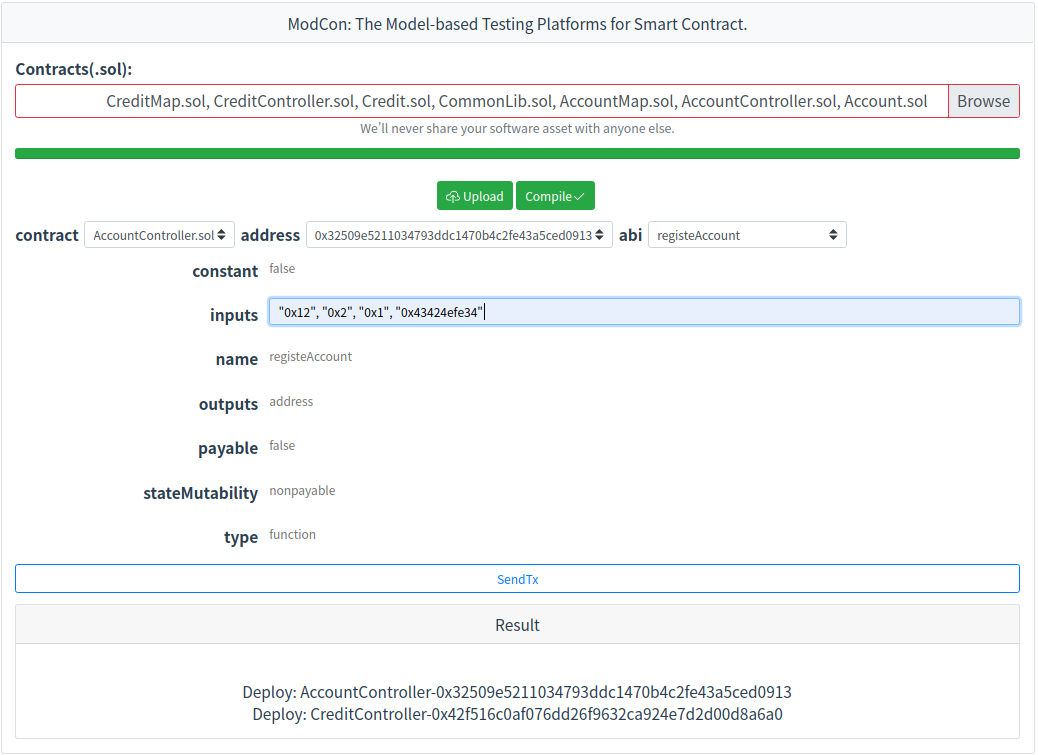
\includegraphics[width=0.90\columnwidth]{Figures/Chapter3/modcon-home.png}
	\caption{Smart contract deployment and setup.}
	\label{fig:modcon-home}
\end{figure}

\paragraph{Contract Setup}
First, users are to upload all relevant smart contract source files, which are then automatically
compiled and deployed onto the blockchain network.
%If there is no compilation error, users can deploy these smart contracts following the on-screen
%guidance.
Once the contracts are successfully deployed, users can directly interact with them by sending
transactions, and the transaction receipts are displayed on the result pane below.
For example, as shown in \cref{fig:modcon-home}, seven contracts related to the \wecredit
application (i.e., \code{Account}, \code{AccountController}, \code{Credit},
\code{CreditController}, ...) had been uploaded to \modcon.
\code{AccountedController} and \code{CreditController} were deployed at addresses,
``\code{0x325...913}'' and ``\code{0x42f...6a0}'', respectively.
One transaction, calling the \code{registerAccount} function, was sent to \code{AccountController}
to create an account which would be used to hold credit instances.
The target contracts' information, including the ABIs and deployment details, are cached and will
be used for test case generation in a later stage.

\begin{figure}[t]
	\centering
	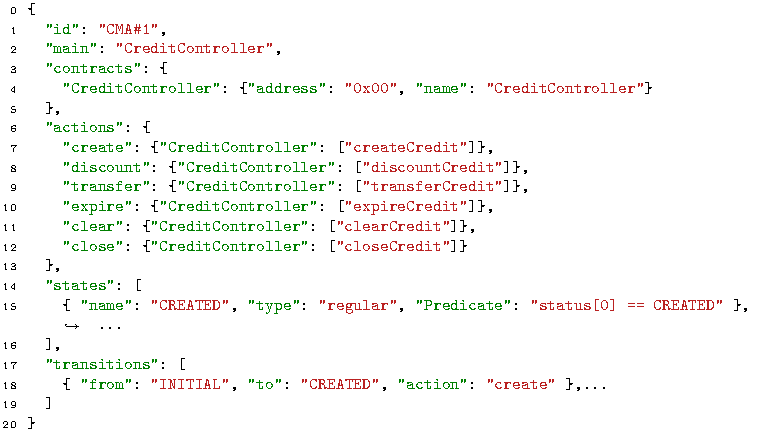
\includegraphics[width=0.9\columnwidth,trim=0 10pt 0 10pt, clip]{Figures/Chapter3/modelSpecification.pdf}
	\caption{User-configured model specification.}
	\label{fig:specification}
\end{figure}

\paragraph{Model Specification}
\Cref{fig:specification} shows an abridged test-model specification for the \wecredit application, which user can customize for his/her applications.
%The specification is explained as follows.
The ``\code{id}'' and ``\code{main}'' fields indicate the model identifier and the entry contract,
respectively.
The ``\code{contracts}'' field lists all relevant contract dependencies required in the test model.
The ``\code{states}'' and ``\code{transitions}'' fields jointly define a state machine model for
the target application.
The ``\code{actions}'' field establish a mapping between functions from the contract implementation
and the actions that can be taken to perform state transitions.

\begin{figure}[t]
	\centering
	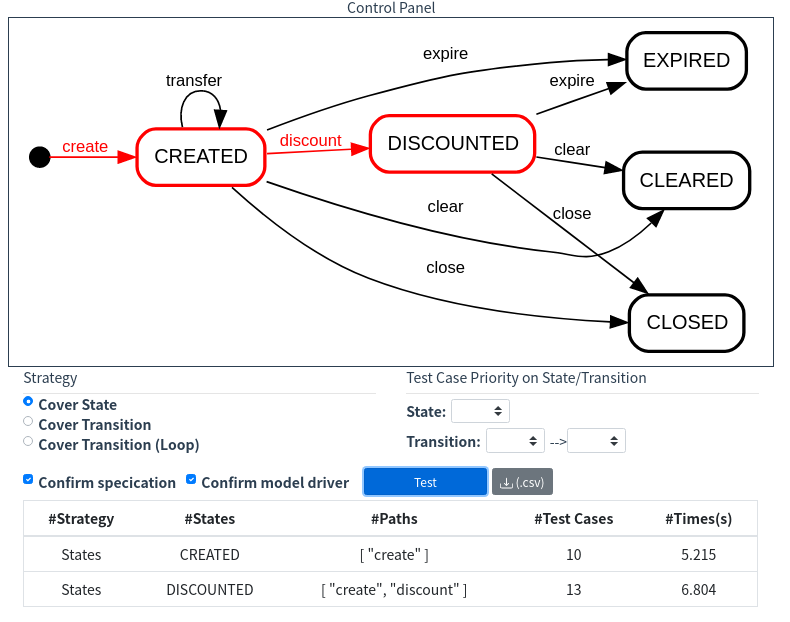
\includegraphics[width=.79\columnwidth]{Figures/Chapter3/modcon-test.png}
	\caption{Test generation control panel.}
	\label{fig:modcon-test}
\end{figure}


\paragraph{TestGen Configuration}
The test-model specification (i.e., \cref{fig:specification}) provided by users is visualized as a
state machine diagram shown in \cref{fig:modcon-test}.
Users may further customize the test generation process by choosing from the three coverage
strategies: (1) \emph{cover states}, aiming to cover every states,
(2) \emph{cover transitions}, aiming to cover every transitions, and
(3) \emph{cover transitions (loop)}, aiming to cover every transitions including loops.
Based on experiments, covering loop transitions may increase testing costs without covering new
states, but it can help discover corner cases and verify the integrity of the test-model.
In addition, users may prioritize the test generation leaning towards specific states or
transitions.
As shows in \cref{fig:modcon-test}, the ``cover states'' strategy is selected and the states
\code{CREATED} and \code{DISCOUNTED} are covered by $10$ and $13$ test cases, respectively.


\subsection{Back-End Implementation}
\label{sec:backend}
The model-based testing engine consists of three parts: i.e., model analyzer, test generation
engine, and blockchain driver.

\paragraph{Model Analyzer}
%The model analyzer handles basic contract compilation as well as deployment, as well as
%transactions, and
The model analyzer reads the model specification from the front-end and automatically translates it
into a test driver written in JavaScript.
The test driver stipulates how tests should be generated and executed, which is then displayed in
the front-end client for users' confirmation and customization.
For instance, users may insert additional test oracles in the form of pre/post conditions and
assertions.

%\noindent\textbf{Compiling \& Deployment module.}
\paragraph{TestGen Engine}
The test generation (TestGen) engine receives testing requests and collects the test-model related
information from the front-end, which includes the confirmed test driver, the coverage strategies,
and the test generation priorities.
The engine first computes all logical transition paths following the specific coverage strategies
and goals using graph searching algorithms.
For example, to reach the \code{CLEARED} state of \wecredit shown in \cref{fig:modcon-test}, the
logical transition paths for different strategies are listed below.

{\small\begin{itemize}[leftmargin=*,topsep=2pt]
		\item Cover states: INITIAL $\rightarrow$ CREATED $\rightarrow$ CLEARED.
		\item Cover transitions: INITIAL $\rightarrow$ CREATED $\rightarrow$ CLEARED; INITIAL $\rightarrow$
		CREATED $\rightarrow$ DISCOUNTED $\rightarrow$ CLEARED.
		\item Cover transitions (loop): INITIAL $\rightarrow$ CREATED $\rightarrow$ CREATED $\rightarrow$
		CLEARED;
		INITIAL $\rightarrow$ CREATED $\rightarrow$ CREATED $\rightarrow$ DISCOUNTED $\rightarrow$ CLEARED.
\end{itemize}}

The TestGen engine ranks these logical transition paths based on the order defined by the test
case priorities, and then generates concrete test cases (with concrete input values and environment
settings) corresponding to each logical transition path.
The generation of concrete input values adopts standard
techniques, such as the mutation-based method in ContraMaster~\cite{wang2019vultron,wang2019oracle},
with seed pools for different input types.
Built upon the blockchain driver, the TestGen engine sends these concrete test cases to blockchain
platforms for execution and monitors the execution status at the same time.
The engine keeps generating test cases for execution until the maximum time budget or failure
limit is reached.
During test execution, the engine reports the testing results back to the front-end client, which
displays the current progress in real-time.

%\lsw{Do we need to mention how the concrete test cases are generated? Maybe one or two sentences?}\liu{The engine generates concrete test input values using a random method, where all test cases to generate share same random seeds pool because for model-driven smart contracts, along one logical transition path, test cases to different transition are highly related.}


\paragraph{Blockchain Driver}
The blockchain driver directly interacts with the blockchain networks for contract deployment and
establishes a transaction interface with the networks.
Currently, \modcon supports two blockchain platforms, namely, Ethereum and FISCO BCOS.
It can easily be extended to other blockchain platforms.
%The instances can be indexed from contract name without much effort, and the driver ensures that the indexed are the latest instance of contract.


\section{Evaluation}
\label{sec:eval}

In this section, we evaluate \modcon on the \wecredit smart contract application from \company and
the \code{BlindAuction} contract used by FSolidM~\cite{mavridou2018designing}, a state machine
based smart contract code generator.

%The case \code{StateMachine} from official Solidity document are also evaluated.
We manually constructed their model specifications with the help from the contract developers and
the related documentation.
The experiments were conducted on a desktop computer with Ubuntu 18.10 OS, an Intel Core i5 $2.50$~GHz processor and $8$GB RAM.
All cases were evaluated on the FISCO BCOS blockchain.

\begin{figure}[t]
	%	\label{fig:cma}
	\centering
	
	\begin{subfigure}[b]{0.47\columnwidth}
		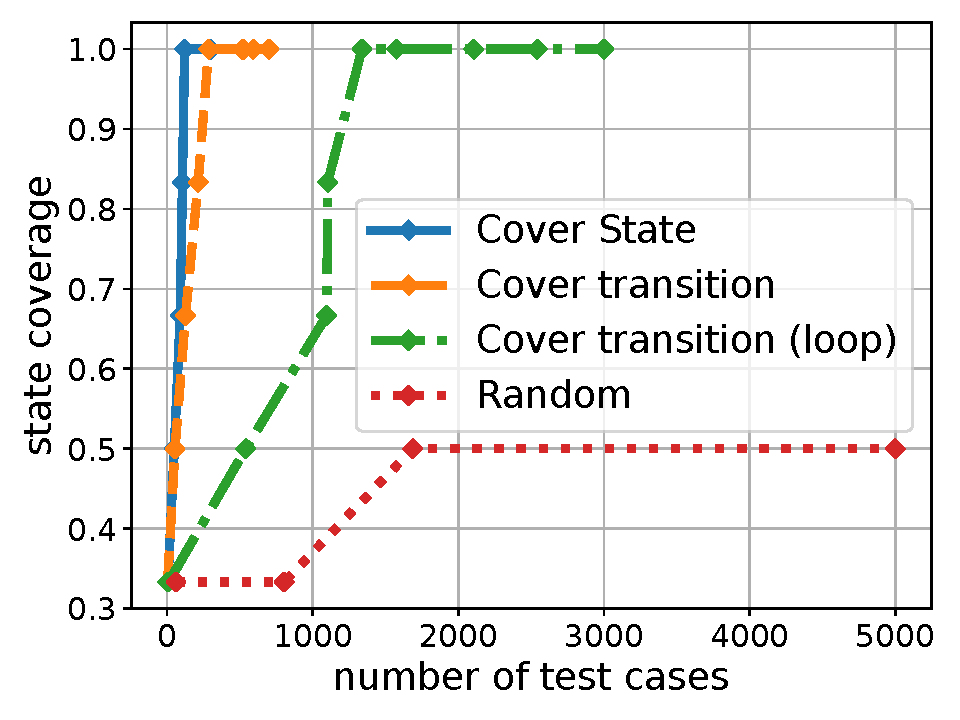
\includegraphics[width=\columnwidth]{Figures/Chapter3/CMA-state-coverage.pdf}
		\caption{\wecredit: state cov.}
		\label{fig:cma-state}
	\end{subfigure}
	\begin{subfigure}[b]{0.47\columnwidth}
		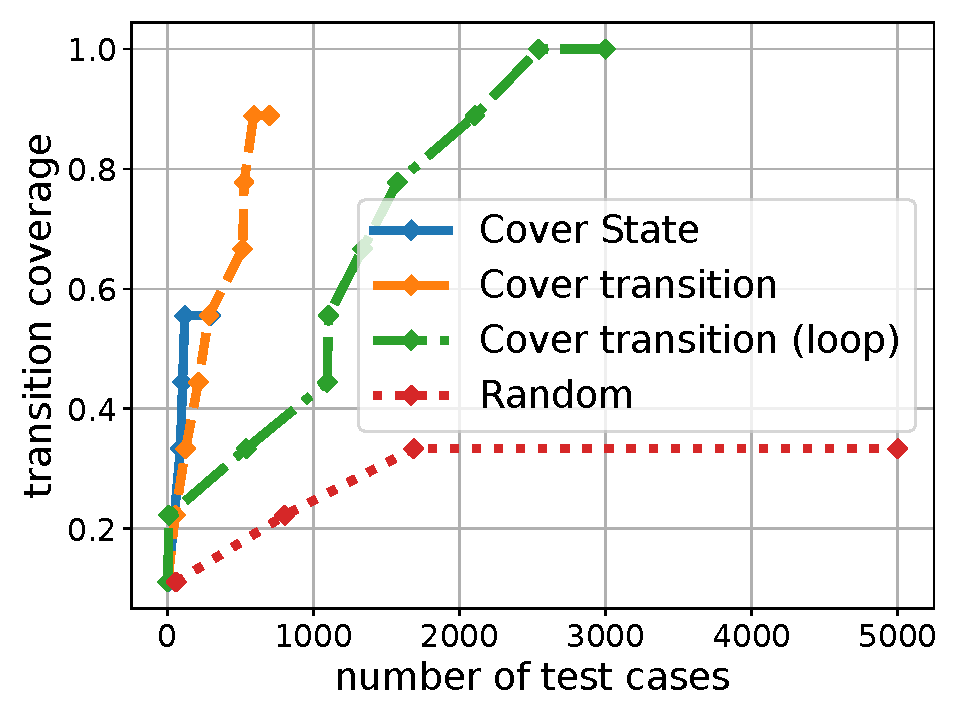
\includegraphics[width=\columnwidth]{Figures/Chapter3/CMA-transition-coverage.pdf}
		\caption{\wecredit: transition cov.}
		\label{fig:cma-transition}
	\end{subfigure}
	\begin{subfigure}[b]{0.47\columnwidth}
		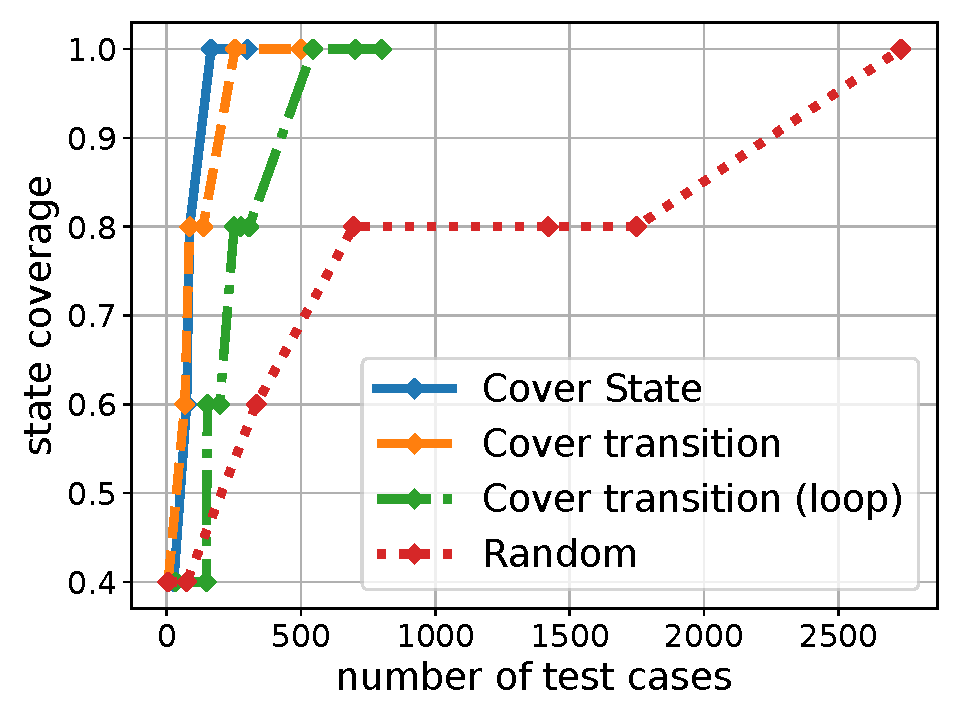
\includegraphics[width=\columnwidth]{Figures/Chapter3/BlindAuction-state-coverage.pdf}
		\caption{\code{BlindAuction}: state cov.}
		\label{fig:auction-state}
	\end{subfigure}
	\begin{subfigure}[b]{0.47\columnwidth}
		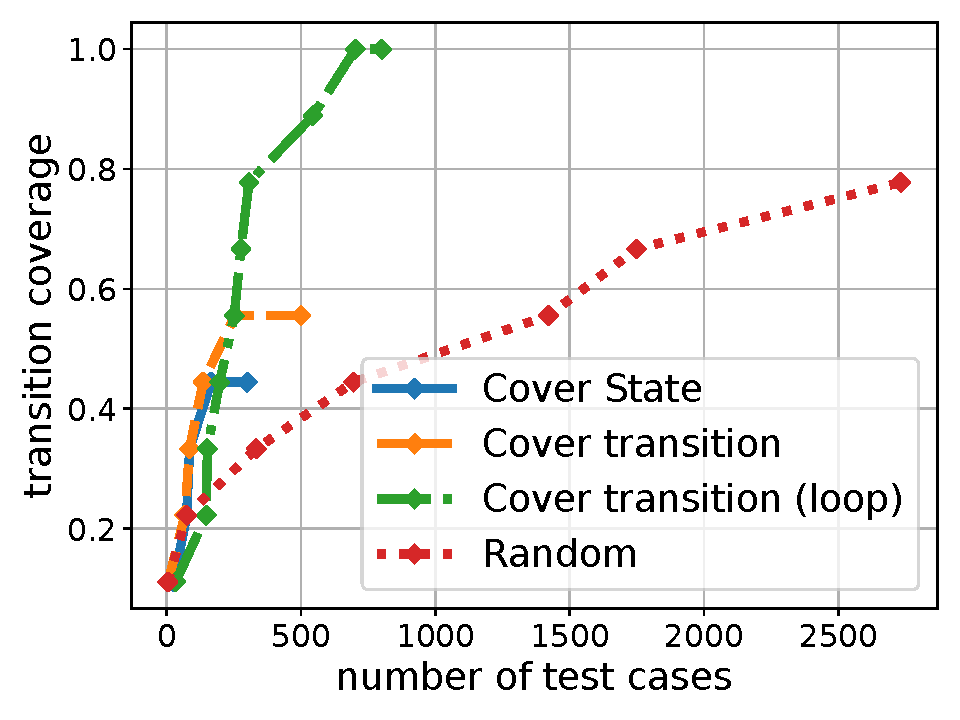
\includegraphics[width=\columnwidth]{Figures/Chapter3/BlindAuction-transition-coverage.pdf}
		\caption{\code{BlindAuction}: transition cov.}
		\label{fig:auction-transition}
	\end{subfigure}
	\caption{State and transition coverage achieved per test for \wecredit and
		\code{BlindAuction}.}\label{fig:coverage}
\end{figure}

%\begin{figure}[ht]
%%	\label{fig:blindAuction}
%	\centering
%
%	\caption{State and transition coverage of BlindAuction.}
%\end{figure}

\Cref{fig:coverage} shows the evaluation results.
The vertical and horizontal axes represent the state/transition coverage and the number of test
cases, respectively.
We examined aforementioned three coverage strategies and compared the results of \modcon with random
testing.
Among these strategies, the results show that the cover state strategy first reaches all states
of both \wecredit and \code{BlindAuction}, while the strategy to cover transition including loops
has the potential to reach all states and explore more transitions at the cost of more test cases.
All of the three proposed strategies achieve much higher state and transition coverage than random
testing, which shows that random testing is not suitable to deal with enterprise smart contract applications.
Random testing achieves lower state and transition coverage in \wecredit than those in
\code{BlindAuction}, because the former is of higher complexity in its business logic and state encoding than the latter.
%has more states and transitions than the latter.
For example, \wecredit uses a bit-vector of more than 11 bits as its function input or to encode the
$\mathit{STATUS}$, and blindly enumerating bit-vector values is extremely inefficient.

In our experiments, \modcon was able to reach all states and transitions for each case within about
500 test cases.
This is mainly because of the guidance from the test-model, which makes \modcon effective on
enterprise smart contract applications such as \wecredit.
Additionally, with the test-model specification, \modcon allows users to define test oracles in the
generated test driver.
For example, the specification of \wecredit requires \code{CLOSED}, \code{CLEARED}, and
\code{EXPIRED} to be final states, which means no transition shall be made once the system falls
into one of the three states.
We insert this specification as a test oracle into the test driver and discovered violations
against it in the original implementation of \wecredit.
The transitions between \code{EXPIRED}, \code{CLOSED}, and \code{CLEARED} were possible due to an
implementation error.
We reported this error to the \wecredit developer team from \company, and they confirmed it to be a
real bug.
The demonstration video of \modcon, along with more cases and experiment results, can be accessed at: \modconurl.

\section{Related Work}
\label{sec:related_work}

%Smart contract development is very different from traditional programming such that developers
%tend
%to write vulnerable smart
%contracts~\cite{delmolino2016step,atzei2016survey,wohrer2018smart,ellul2018runtime}.
Most of the existing testing and analysis tools focus on the security issues of Ethereum smart
contracts.
Oyente~\cite{oyente,luu2016making} is one of the first static analyzer detecting security
vulnerabilities in smart contracts based on symbolic execution.
It searches for violations of predefined security properties without actually executing the
contract program.
Other notable static security analysis tools include Zeus~\cite{kalra2018zeus},
Mythril~\cite{mythril}, sCompile~\cite{chang2018scompile}, and Securify~\cite{tsankov2018securify}.
In contrast, the dynamic tools instrument either the contract code or the Ethereum Virtual Machine
(EVM) and observe anomalies during runtime execution.
ContractFuzzer~\cite{jiang2018contractfuzzer} is the earliest dynamic fuzz testing tool aiming a
number of common vulnerability types, including the reentrancy, exception disorder, block
dependency, etc.
Other fuzzing tools follow similar principles: e.g., Reguard~\cite{liu2018reguard},
ContraMaster~\cite{wang2019vultron,wang2019oracle}, and sFuzz~\cite{nguyen2020sfuzz}.
% arose as the first industrial security analysis tool for Ethereum smart contracts, which combined
% concolic analysis and taint analysis with control flow checking to detect  nearly 30 classes of
% vulnerabilities.
%Also, there are many works resorting to programming analysis technique to detect the
%vulnerabilities of smart contract~\cite{SmartCheck} and empirical
%analysis~\cite{parizi2018empirical} to the tools mentioned above.
These tools are not designed for testing functional correctness, and as mentioned in \cref{sec:intro}, they are not suitable for enterprise smart contract applications
either.

There are several recent works on the functional correctness of Ethereum smart contracts.
VeriSol~\cite{born2020formal} relies on formal verification to check the semantic conformance
between a contract implementation and its workflow policy.
The policy is provided by users, describing the high-level workflow of the application in a style
similar to our model specifications.
FSolidM~\cite{mavridou2018designing} and VeriSolid~\cite{Mavridou2019} both aim to facilitate the
creation of correct-by-design contracts, with emphases on the security and functional aspects,
respectively, 
where a finite state machine is used as the contract specification to capture the expected system behaviors.
\modcon is based on the idea of model-based testing~\cite{utting2012taxonomy}, which uses an explicit
abstract model of the target contract to automatically derive tests.
It serves as a complement to other static validation/construction techniques in providing more
flexible and accurate quality assurance solutions.

\section{Conclusion}
\label{sec:conclude}

In this paper, we described the architecture of \modcon, its user interface, and prominent features.
We also demonstrated the effectiveness of it on real smart contract applications from \company.
The model-based testing capability of \modcon enables it to generate higher-quality test cases for
enterprise smart contracts from permissioned and consortium blockchains.
%Its Web-based interface allows users to easily access the testing services.
%In the future, we plan to extend \modcon's testing capabilities by supporting more blockchain
%platforms, testing strategies and specification templates.
\chapter{Future Work}
\chaptermark{Future Work}
\label{ch:futurework}

%\section{Introduction (Need to rewrite)}
%\label{sec:Introduction}


Smart contracts are computer programs running atop blockchain platforms to manage large sums of
money, carry out transactions of assets, and govern the transfer of digital rights between multiple
parties.
Ethereum~\cite{Ethereum} and EOS~\cite{EOS} are among the most popular blockchain platforms which
support smart contracts and have them applied in many areas, such as finance, supply chain,
identity management, games, etc.
As of April 2021, there are over 10 millions smart contracts deployed on Ethereum, which is a 10 fold
increase since just one years ago~\cite{Etherscan}.
These smart contracts have enabled about 3.1 K decentralized applications (DApps) serving 80 K
daily users.
%\todo[inline]{talk about contract security.}


Smart contracts deployed on permissionless blockchains, such as Ethereum, are accessible to any
user in a trust-less environment.
Therefore, most smart contract applications implement access control policies to protect their
valuable assets from unauthorized accesses.
The correctness of such policies is critical for maintaining smart contract security.
For example, suicidal contracts~\cite{nikolic2018finding} is a class of vulnerable smart contracts
without proper access control to the ``\texttt{selfdestruct}'' operations, which appear in around
20\% of unique smart contracts~\cite{oyente}.
Another high-profile victim due to vulnerable access control policy is the Parity Wallet.
The wallet was hacked through two different attack vectors resulting in the stolen of \$30M USD and
the frozen of \$100M USD, respectively.
The Parity Wallet consumes a library contract, called WalletLibrary, to implement the basic
functionality of a wallet.
Anybody can deposit money into the wallet, but only the contract owner can withdraw the funds.
The first attack vector exploited the unprotected initialization function to set the attacker as
the contract owner and finally withdrew a large sum of money deposited by other wallet users.
The root cause of this attack is that an unauthorized user can bypass the contract rule rather than
the intended user access.

A difficulty in validating the conformance to such policies, i.e., whether the contract
implementation adheres to the expected behaviors, is the lack of policy specifications. The
current practice is to implement intended access control policies with ad-hoc
Solidity~\cite{solidity} (i.e., the programming languages used to develop Ethereum smart contracts)
idioms, such as the ``\texttt{require}''statements, to check if the address of a user is in a
predefined whitelist.
Many security vulnerabilities mentioned earlier are results from this ad-hoc approach.
In particular, when the number of roles and the complexity of access patterns increase, it becomes
fairly easy for contract developers to make mistakes and introduce bugs causing security
vulnerabilities.

\begin{figure}[t]
	\centering
	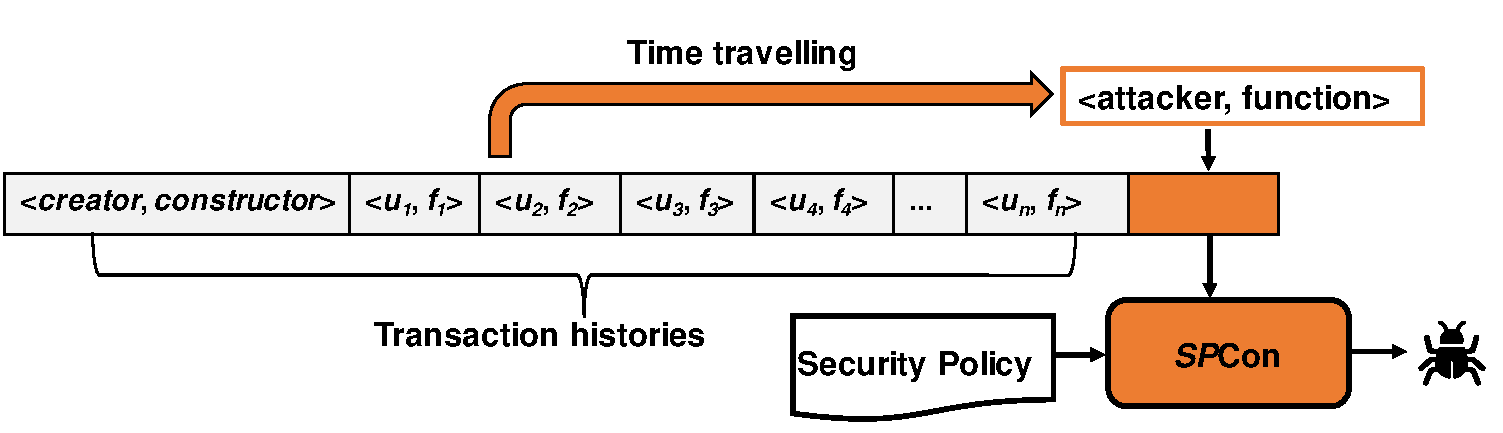
\includegraphics[width=\linewidth]{Figures/Chapter4/SPconIllustration-crop.pdf}
	\caption{Illustration of the time-travel-based security policy validation.}
	\label{fig:time-travel}
\end{figure}

In this paper, we would like to address this problem by relying on past transactions of a contract
to recover a \emph{likely} access control model, which can then be validated against various
security rules and identify potential bugs related to user permissions.
We plan to implement a security policy validator powered by ``time traveling'' through transaction
histories.
As is shown in \cref{fig:time-travel}, the key idea is that, because of the transparency and
immutability of blockchain transactions, the transaction histories of a smart contract application
from its initial deployment up to today are always available on the blockchain.
The historical transactions of a smart contract contain benign user behaviors, assuming the
contract is not yet attacked by any malicious party.
Due to the unique nature of DApps, we can safely assume that the history of a smart contract is
\emph{clean}, if it is still \emph{alive}, i.e., not being destructed or abandoned.
Therefore, we are able to reverse engineer an access control model which is permissible enough to
subsume all historical transactions.
Since historical transactions only under-approximate the behaviors allowed by the contract
implementation, by validating the recovered model against the actual contract implementation, we
will be able to discover discrepancies, indicating potential future violations of security policies.
%\part{Coordinated Estimation} %
\chapter{Conclusion} % Main chapter title
\chaptermark{Conclusion}  % replace the chapter name with its abbreviated form
\label{ch:conclusion} % Change X to a consecutive number; for referencing this chapter elsewhere, use \ref{ChapterX}

This report compiles the published works that I have done on model based testing of smart contracts, automatic fairness verification of smart contracts.
The promising results of these works provide strong support for the efficiency and capability of model-based testing compared to existing testing methods 
and for the importance of fairness problem related to smart contracts, which usually deviates from the expectation of novice contract users respectively.
The future work on finding permission bugs via time travel on transaction history of smart contracts has also been briefly illustrated and will be finished in the near future.
Meanwhile, a big picture of the framework to enforce both security and fairness of smart contracts remains a quite challenge which I will also explore further.
%\chapter{Future Work} % Main chapter title
\chaptermark{Future Work}  % replace the chapter name with its abbreviated form
\label{ch:future_work} % Change X to a consecutive number; for referencing this chapter elsewhere, use \ref{ChapterX}

%\chapter{The Access Control of Smart Contracts}
\section{Access Control Patterns}
\section{State-Based Access Control}
\section{Role-Based Access Control}
\section{Case Study}



%----------------------------------------------------------------------------------------
%	THESIS CONTENT - APPENDICES
%----------------------------------------------------------------------------------------

\addtocontents{toc}{\vspace{0.8em}} % Add a gap in the Contents, for aesthetics

\appendix % Cue to tell LaTeX that the following 'chapters' are Appendices

% Include the appendices of the thesis as separate files from the Appendices folder
% Uncomment the lines as you write the Appendices

% %!TEX root=../mythesis.tex
% Appendix A

\chapter{Proofs for Part I} % Main appendix title

\label{AppendixA} % For referencing this appendix elsewhere, use \ref{AppendixA}

%\lhead{Appendix A. \emph{Appendix Title Here}} % This is for the header on each page - perhaps a shortened title
\section{Proof of Lemma}
\label{pf:ApprGradSys}

$$\psi^{av}(\theta)=\frac{1}{T}\int^{T}_0[\psi(\theta+\mu(\tau))+C]\otimes\frac{\mu(\tau)}{a}d\tau$$ 



\section{Proof of another Lemma}
\begin{equation}
\begin{aligned}
\gamma_1(\left\|x\right\|)\leq W(t,x)\leq \gamma_2(\left\|x\right\|)\\
\frac{\partial{W}}{\partial{t}}+\frac{\partial{W}}{\partial{x}}\phi(t,x,0)\leq-\gamma_3(\left\|x\right\|)
\end{aligned}
\end{equation}

%\input{./Appendices/AppendixB}

\cleardoublepage    % start a new page


\backmatter

%----------------------------------------------------------------------------------------
%	BIBLIOGRAPHY
%----------------------------------------------------------------------------------------

\label{Bibliography}
\setstretch{1}
\bibliographystyle{unsrtnat}
%\bibliographystyle{ACM-Reference-Format}
%\bibliography{bibexport}
\bibliography{References/ref}

\end{document}
